% Template file for a standard thesis
\documentclass[11pt]{isuthesis}
%\usepackage[spanish,english]{babel}
%\addto\captionsenglish{
%\renewcommand{\chaptername}{CHAPTER\ }
%}
\usepackage[pdftex]{graphicx}
% Standard, old-style thesis
\usepackage{isutraditional} \chaptertitle
% Old-style, thesis numbering down to subsubsection
\alternate
\usepackage{rotating}
% Bibliography without numbers or labels
\usepackage{natbib}

\RequirePackage[OT1]{fontenc}
\RequirePackage{amsthm,amsmath,amsfonts}
\usepackage{tikz}
\usepackage{graphicx}
%\usepackage[caption=false]{subfig}
\usepackage[all]{nowidow}


\newtheorem{prop}{Proposition}

\bibliographystyle{apa}
%\includeonly{titletoc,chapter1}
%Optional Package to add PDF bookmarks and hypertext links
\usepackage[pdftex,hypertexnames=false,linktocpage=true]{hyperref}
\hypersetup{colorlinks=true,linkcolor=blue,anchorcolor=blue,citecolor=blue,filecolor=blue,urlcolor=blue,bookmarksnumbered=true,pdfview=FitB}

\usetikzlibrary{arrows,chains,matrix,positioning,scopes}
%
\makeatletter
\tikzset{join/.code=\tikzset{after node path={%
			\ifx\tikzchainprevious\pgfutil@empty\else(\tikzchainprevious)%
			edge[every join]#1(\tikzchaincurrent)\fi}}}
\makeatother
%
\tikzset{>=stealth',every on chain/.append style={join},
	every join/.style={->}}
\tikzstyle{labeled}=[execute at begin node=$\scriptstyle,
execute at end node=$]
\begin{document}
\DeclareGraphicsExtensions{.jpg,.pdf,.mps,.png}
% Template Titlepage File
\title{Self-exciting spatio-temporal modeling and estimation of count data with applications to modeling the spread of violence}
\author{Nicholas John Clark}
\degree{DOCTOR OF PHILOSOPHY}
%\level{master's}
\mprof{Philip M. Dixon}
%\members{Mary Jones \\ Bjork Petersen}
\notice
% Add these additional lines for a Doctoral Dissertation
\degree{DOCTOR OF PHILOSOPHY}
\level{doctoral}
\format{dissertation}
\committee{4}
\members{Mark Kaiser \\ Jarad Niemi \\ Zhengyuan Zhu \\ Ulrike Genschel}
% Add these additional lines for a Doctoral Dissertation
%\degree{DOCTOR OF PHILOSOPHY}
%\level{doctoral}
%\format{dissertation}
%\committee{4}
%\members{Mary Jones \\ Bjork Petersen \\ Sam Anders \\ Harold Jones}
% Add these additional lines for a Creative Component
% - also comment out the \maketitle command
%\format{Creative Component}
%\submit{the graduate faculty}
\maketitle

% Optional thesis dedication
\chapter*{DEDICATION}

Dedication

\pdfbookmark[1]{TABLE OF CONTENTS}{table}
\tableofcontents
\addtocontents{toc}{\def\protect\@chapapp{}} \cleardoublepage \phantomsection
\addcontentsline{toc}{chapter}{LIST OF TABLES}
\listoftables
\cleardoublepage \phantomsection \addcontentsline{toc}{chapter}{LIST OF FIGURES}
\listoffigures
% Comment out the next line if NOT using chaptertitle
\addtocontents{toc}{\def\protect\@chapapp{CHAPTER\ }}
%Optional Acknowledgements
\cleardoublepage \phantomsection
\specialchapt{ACKNOWLEDGEMENTS}
Acknowledgments 
%Optional thesis abstract
\cleardoublepage \phantomsection
\specialchapt{ABSTRACT}

In this dissertation, we provide statistical models and inferential techniques for analyzing the number of violent or criminal events over space and time.  Our research focuses on a class of models we refer to as self-exciting spatio-temporal models.  These are a class of parametric models that allow for dependence in a latent structure as well as dependence in the data model combining what is sometimes referred to as observation drive and parameter drive models.  This class of models has use in modeling data where there is an expected repeat or near-repeat victimization that is common in the study of criminology.  In Chapter 2 we present the spatially correlated self-exciting model and the reaction-diffusion self-exciting model to analyze the number of violent events in different regions in Iraq.  We also demonstrate how Laplace approximations can be used to conduct efficient Bayesian inference.  We further show how the choice of the latent structure matters in this problem.  In Chapter 3 we generalize the spatially correlated self-exciting model and show how it extends the classic integer generalized auto-regressive conditionally heteroskedastic, or INGARCH, model to account for spatial correlation and improves the second order properties of the INGARCH model.  We refer to this new class of models as the spatially correlated INGARCH, or SPINGARCH, model.  We show how the spatially correlated self-exciting model is similar to the SPINGARCH(0,1) model.  Finally in Chapter 4 we present an extended Laplace approximation algorithm and demonstrate empirically how the extended Laplace approximation method eliminates a bias that exists in the Laplace approximation method for one of the parameters in the spatially correlated self-exciting, or SPINGARCH(0,1), model. 
\newpage
\pagenumbering{arabic}
% Chapter 1 of the Thesis Template File
\chapter{Introduction}
The statistical modeling of violence has generally neglected to properly account for spatial and temporal correlation.  In \cite{ratcliffe2010crime}, the argument is made that potential temporal correlation is often ignored in the statistical modeling of crimes whereas in examples such as \cite{mohler2013modeling} spatial correlation is ignored.  One of the principal challenges is that there are few available statistical models for count data that both offer a mechanism for capturing spatial-temporal correlation as well as result in meaningful inference.  The commonly used Poisson-Log Normal model, for example, only allows limited data correlation as described in \cite{aitchison1989multivariate}.  Furthermore, this method of modeling assumes that, in the terminology of \cite{cox1981statistical}, large scale structure in the model is parameter-driven.  On the other hand, criminologists have shown the presence of repeat victimization in \cite{johnson1997new} and \cite{johnson2007space}.  To properly account for this phenomena, a statistical model should consider observation-driven structure, commonly referred to as self-excitement.

In this dissertation, we propose a new class of statistical models that accounts for self-excitement in the modeling of the spread of violence.  Motivating our work is the assumption that violence at a given space-time region can arise both due to repeat victimization as well as  exogenous factors.  This assumption allows us to formulate a class of parametric model for the counts of violence that has flexible second order properties and can be fit using standard Bayesian software.

\section{Spatio-temporal counts of violent events}

The number of crimes or other violent events is usually aggregated over a fixed space-time lattice and presented as count data.  For example, we use two primary datasets throughout this dissertation that are both aggregated due to both privacy issues as well as convenience.  The first dataset is from the Global Terrorism Database (\cite{lafree2007introducing}).  We specifically look at the incidents in Iraq from 2003-2010.  During this time period violence was common and it was difficult to distinguish between crime and terrorism.  For example, figure \ref{IZSpread} depicts the monthly counts of US government reported violent incidents in Iraq aggregated over province during this time period.  In figure \ref{IZSpread} the violence appears to spread out of the center of the country.  We further consider crime in Chicago freely available from the city of Chicago (\href{https://data.cityofchicago.org/Public-Safety/Crimes-2001-to-present}{https://data.cityofchicago.org/Public-Safety/Crimes-2001-to-present}).  From here we use, for example, the number of burglaries per census block in the south side of the city.  As shown in figure \ref{ChiSpread}, the spatial correlation is much less obvious than in Iraq, however as we will show it is still present in the data.

\begin{figure}[h] % figuur 1
	\begin{center}
		\vspace{6pc}
		\includegraphics[width=.8 \linewidth]{Iraq2.pdf}
		\isucaption[Spread of violence in Iraq in 2004]{The spread of the log-count of violence in Iraq over discrete regions and discrete times.}
		\label{IZSpread}
	\end{center}
\end{figure} 



\begin{figure}[h] % figuur 1
	\begin{center}
		\vspace{6pc}
		\includegraphics[width=.8 \linewidth]{ChiBurg.pdf}
		\isucaption[Spread of burglaries in the south side of Chicago]{Spread of burglaries in the south side of Chicago in 2011.}
		\label{ChiSpread}
	\end{center}
\end{figure} 




\section{Self-excitement in a statistical model}
The models we present rely on the notion of self-excitement.  The general idea of self-excitement in a statistical model is not new.  It originates from \cite{hawkes1971spectra} work in point process data where the intensity of a Poisson process, $\lambda(t)$ is assumed to depend both on $t$ as well as past realizations of the process
\begin{equation}
\lambda(t)=\nu + \int_{0}^t g(t-s)N(ds),\quad t>0.
\end{equation}
Here $g(t)$ can be thought of as a triggering function that generally decays over time.  In this manner, an observed event today increases the probability of a subsequent event occurring the following day.  In the modeling of violence this is the notion of repeat, or near repeat victimization shown to exist in burglaries in \cite{johnson1997new} and \cite{johnson2007space}. 

The resulting statistical model using self-excitation is doubly stochastic as $\int_{0}^t g(t-s)N(ds)$ depends on a random variable, the number of events between time $t$ and $t-s$.  However, as demonstrated in \cite{mohler2013modeling}, there may be other forms of latent variation in the intensity function.  In that manuscript the authors demonstrated how the modeling of crimes in Chicago as well as violence in Iraq is improved through the addition of a latent auto-regressive term.  In particular, they assumed that the number of violent events, $y_t$, between $t$ and some fixed $t-\Delta t$ follows a Poisson distribution with expectation given by
\begin{align}
& \lambda_t  =\exp(x_t)+\sum_{t>j} \theta^{t-j} y_j\\
& \boldsymbol{x} \sim \mbox{Gau }(\boldsymbol{0},\Sigma)\\
& \Sigma_{t,j} =\sigma^2 a^{|t-j|}.
\end{align}
That is, the expected number of violent events is a linear combination of a discrete self-excitement term and a log-Gaussian Auto-Regressive (1) model.  While this improved the fit, clearly spatial correlation was ignored.

\section{Self-exciting spatio-temporal parametric models}

Historically, the modeling of spatial-temporal count data has relied on the assumption that the log expected counts can be modeled as a latent Gaussian random variable (e.g. in \cite{python2016bayesian}).  In our belief this is overly restrictive and makes an realistic assumption that the counts are conditionally independent given a latent process and does not account for the possibility of self-excitement.  Attempts at accounting for self-excitement generally fail to address the spatial correlation as in \cite{mohler2013modeling} or estimate it non-parametrically as in \cite{mohler2011self}.  

In this dissertation we consider the impacts of combining self-excitement with spatial and spatio-temporal latent structures.  In Chapter \ref{AoAS} we propose two different latent structures resulting in a spatially correlated self-exciting statistical model and a reaction diffusion self-exciting statistical model.  We further demonstrate an efficient methodology for conducting Bayesian inference based on Laplace approximations and apply the methodology to the counts of violent events in Iraq.

In Chapter \ref{JASA} we extend the spatially correlated self-exciting model and demonstrate similarities between this model and a relatively recent discrete valued time series model called the integer generalized autoregressive conditional heteroskedasticity, or INGARCH, model.  In that spirit, we refer to the resulting model as the spatially correlated, or SPINGARCH model.  We demonstrate how the model can be fit using off the shelf software for Bayesian inference.  We further show how the model out performs the INGARCH model in capturing the second order properties of the number of burglaries in the south side of Chicago.

Finally, in Chapter \ref{CSDA}, we present an efficient methodology for Bayesian inference of the spatially correlated self-exciting model (also referred to as the SPINGARCH(0,1) model) based on an extended Laplace approximation.  We show how for a large range of the parameter space the extended Laplace approximation matches Markov chain Monte Carlo (MCMC) based techniques.  



\chapter{Modeling and Estimation for Self-Exciting Spatio-temporal Models of Terrorist Activity}\label{AoAS}
\begin{center}
	Preprint of a manuscript accepted in \textit{The Annals of Applied Statistics}.\\
	Nicholas J. Clark, Philip M. Dixon
\end{center}
\section*{Abstract}
Spatio-temporal hierarchical modeling is an extremely attractive way to model the spread of crime or terrorism data over a given region, especially when the observations are counts and must be modeled discretely.  The spatio-temporal diffusion is placed, as a matter of convenience, in the process model allowing for straightforward estimation of the diffusion parameters through Bayesian techniques.  However, this method of modeling does not allow for the existence of self-excitation, or a temporal data model dependency, that has been shown to exist in criminal and terrorism data.  In this manuscript we will use existing theories on how violence spreads to create models that allow for both spatio-temporal diffusion in the process model as well as temporal diffusion, or self-excitation, in the data model.  We will further demonstrate how Laplace approximations similar to their use in Integrated Nested Laplace Approximation can be used to quickly and accurately conduct inference of self-exciting spatio-temporal models allowing practitioners a new way of fitting and comparing multiple process models.  We will illustrate this approach by fitting a self-exciting spatio-temporal model to terrorism data in Iraq and demonstrate how choice of process model leads to differing conclusions on the existence of self-excitation in the data and differing conclusions on how violence spread spatially-temporally in that country from 2003-2010.

\section{Introduction} 
A typical spatio-temporal model consists of three levels, a data model, a process model, and a parameter model.  A common way to model data then is to assume the data model, $Y(\cdot)$, is conditionally independent given the process model $X(\cdot)$. For example, if observations take place at areal regions, $\boldsymbol{s_i}$, at discrete time periods, $t$, and $Y(\boldsymbol{s_i},t)$ are counts, a common model is $Y(\boldsymbol{s_i},t)|X(\boldsymbol{s_i},t)\sim \mbox{Pois}(\exp(X(\boldsymbol{s_i},t)))$.  The spatio-temporal diffusion structure is commonly then placed on the process model which commonly is assumed to have a Gaussian joint distribution of $\boldsymbol{X}\sim \mbox{Gaus}(\boldsymbol{0},Q^{-1}(\theta))$.  The majority of analysis of these models is done using Bayesian techniques requiring a further parameter model for $\theta$.  The challenge in these models is, then, determining an appropriate structure for $\boldsymbol{Q}^{-1}(\theta)$ or $\boldsymbol{Q}(\theta)$.  If both the covariance and the precision is chosen to be too dense inference quickly becomes impossible due to the size of $\boldsymbol{Q}^{-1}(\theta)$.  In spatio-temporal models it is quite common for the dimension of $\boldsymbol{Q}$ to be larger than, say, $10^4\times 10^4$.  A thorough overview giving many examples of this method of modeling is given in \cite{cressie2015statistics}.

In modeling terrorism or crime data one possibility is to use an extremely general spatio-temporal process model to capture variance not explained through the use of covariates.  For example \cite{python2016bayesian} use a Matern class covariance function over space and an AR(1) process over time.  They then use covariates to test the impact of infrastructure, population, and governance.  The general spatio-temporal process models used, in this case, has an extremely sparse precision structure greatly aiding in computations.

While diffusion in spatio-temporal models is often modeled through a latent process, more recent models describing the spread of violence have incorporated self-excitation, or spatio-temporal diffusion that exists linearly in the data model itself.  Self-excitation is the theory that in terrorism, or crime, the probability of an event occurring is a function of previous successful events.  For instance \cite{mohler2011self} demonstrate that burglars are more likely to rob locations that have previously, successfully, been robbed.  \cite{mohler2013modeling} derived a class of models that allowed for temporal diffusion in both the process model as well as the data model and demonstrated how the two processes were identifiable.

In the modeling of terrorism data \cite{lewis2012self}, \cite{porter2012self}, and \cite{mohler2013modeling} have all successfully used the self-excitation approach to model.  Most recently, \cite{tench2016spatio} used a likelihood approach for temporal modeling of IEDs in Northern Ireland using self-excitation.  However, in these papers, the existence and analysis of self-excitation was the primary objective and any process model dependency was either ignored or treated as a nuisance.  The one exception is in \cite{mohler2013modeling} where a temporal only model was assumed for the process model and inference was conducted on both the process model dependency and the data model dependency.

In this manuscript, we will consider a spatial and a spatial-temporal process model that allows for self-excitation.  We will present two self-exciting models for terrorist activity that have different process models corresponding to different notions of how terrorism evolves in time and space as well as temporal dependency in the data model to account for self-excitation.  These two models are specific cases of more general spatio-temporal models that allow dependency in both the process model as well as the data model.

We will further show how Laplace approximations similar to their use in Integrated Nested Laplace Approximation, or INLA, an approximate Bayesian method due to \cite{rue2009approximate} can be used to conduct inference for these types of models. We will show, via simulation, how INLA, when appropriately modified, can accurately be used to make inference on process level parameters for self-exciting models and aid analysts in determining the appropriate process model when scientific knowledge cannot be directly applied as in \cite{cressie2015statistics}.  Finally, we will apply this technique to terrorism data in Iraq.  We will show that choice of process model, in this case, results in differing conclusions on the impact of self-excitation in the model.  


\section{Self-Exciting Spatio-Temporal Models}
The use of self-exciting models in both criminal and terrorism modeling has become increasingly popular over the last decade after being originally introduced in \cite{short2008statistical}.  Self-excitement, in a statistical model, directly models copy-cat behavior by letting an observed event increase the intensity (or excites a model) over a specified time or location. Self-exciting models are closely related to Hawkes processes, which are counting processes where the probability of an event occurring is directly related to the number of events that previously occurred. In a self-exciting model, the criminal intensity at a given spatio-temporal location, $(x,y,t)$ is a mixture of a background rate, $\nu$ and self excitement function, $f(\mathcal{H}_{x,y,t})$ that is dependent on the observed history at that location, $\mathcal{H}_{x,y,t}$.  

A common temporal version of a discretized Hawkes process is
\begin{align}
& Y_t\sim \mbox{Pois}(\lambda_t) \\
& \lambda_t = \nu + \sum_{j < t} \kappa (t-j) y_j \nonumber\\
& t \in \{1,2,...T\}
\end{align}

In this example, in order for the process to have finite expectation in the limit, $\kappa(t-j)$ must be positive and $\sum_{i=1}^{\infty} \kappa (i) <1$.  $\kappa (t-j)$ can be thought of as the probability that an event at time $j$ triggers an event at time $i$.

\cite{laub2015hawkes} provides an excellent overview of the mathematical properties of the continuous Hawkes process and the discrete process when $\kappa (t-j)$ is taken to be an exponential decay function.

In \cite{mohler2011self}, $\nu$ was treated as separable in space and time and was non-parametrically estimated using stochastic declustering, while in \cite{mohler2013modeling}, the spatial correlations were ignored and an AR(1) process was used for $\kappa(t)$ and an exponential decay was assumed for the self-excitation.  In terrorism modeling \cite{lewis2012self} used a piece-wise linear function for $\kappa(t)$.  

Here we will first define a general model that allows spatial or spatial-temporal correlation to exist in the process model and positive temporal correlation to exist in the data model to allow for self-excitation.  First define $s_i \in \mathbb{R}^2$, $i \in \{1,2,...,n_d\}$ as locations in a fixed, areal, region. We further define $t \in \{1,2,...,T\}$ as discrete time. The general form of a spatial-temporal self-exciting model is then given in \eqref{eq:gen Model}

\begin{align}
& Y(\boldsymbol{s_i},t)|\mu(\boldsymbol{s_i},t) \sim \mbox{Pois}(\mu(\boldsymbol{s_i},t)) \label{eq:gen Model}\\
& \mu(\boldsymbol{s_i},t) = \exp(X(\boldsymbol{s_i},t)) + \eta Y(\boldsymbol{s_i},t-1) \nonumber \\
& \boldsymbol{X} \sim \mbox{Gau}(\boldsymbol{0},Q^{-1}(\theta))) \nonumber
\end{align}

Comparing the above to the Hawkes process, we now have $\nu$ as a function of space-time and denote it as $X(\boldsymbol{s_i},t)$.  We use the simplest form of self-excitation letting $\kappa(t-j)$ be a point-mass function such that $\kappa(k)=\eta$ for $k=1$ and $\kappa(k)=0$ for $k \neq 1$.  In all cases $Y(\boldsymbol{s_i},t)$ will be discrete, observable, count data.  

To contrast \eqref{eq:gen Model} with a typical spatial model, figure \ref{exc} depicts the expectation for one areal location $(\boldsymbol{s_i},t)$ without self-excitation and with self-excitation as shown in Figure \ref{exc}. In this figure, the lower line shows $\mu(\boldsymbol{s_i},t)$ with $\eta=0$, and the upper line has $\eta=.4$.  The impact of self-excitation is clearly present in time 10-13.

\begin{figure}[h]
	\begin{center} % figuur 1
		\vspace{6pc}
		\includegraphics[width=.5 \linewidth]{Contageon3.pdf}
		\isucaption[ Self-Excitement in a Statistical Model]{This figure shows an example of the expectation of two processes, one with self-excitation and one without.  The bottom line is the expectation of a process with no self-excitation, the top has self-excitation of $\eta=.4$. The data realizations are from the process with self-excitation.}
		\label{exc} 
	\end{center}
\end{figure}



\subsection{Spatially Correlated Self-Exciting Model}

In the first example of \eqref{eq:gen Model} we assume the background intensity rate, $X(\boldsymbol{s_i},t)$ has only spatial correlation.  This model is motivated through the assumption that the latent dependency, $X(\boldsymbol{s_i},t)$, is as a continuous measure of violent tendency at region $s_i$ at time period $t$ and regions that are closer together in space are assumed to share common characteristics.  

Next, define $N(\boldsymbol{s_i})$ as the neighborhood of location $s_i$ where two regions are assumed to be neighbors if they share a common border.   $|N(\boldsymbol{s_i})|$ is the number of neighbors of location $s_i$.  The model for $Y(\boldsymbol{s_i},t)$, or the number of observed violent events at a given space-time location is then given by:

\begin{align}
& Y(\boldsymbol{s_i},t)|\mu(\boldsymbol{s_i},t) \sim \mbox{Pois}(\mu(\boldsymbol{s_i},t)) \label{eq:Full Model}\\
& \mu(\boldsymbol{s_i},t) = \exp(X(\boldsymbol{s_i},t)) + \eta Y(\boldsymbol{s_i},t-1) \nonumber \\
& X(\boldsymbol{s_i},t) = \theta_1 \sum_{\boldsymbol{s_j}\in N(\boldsymbol{s_i})}X(\boldsymbol{s_j},t) + \epsilon(\boldsymbol{s_i},t) \nonumber\\
&\epsilon(\boldsymbol{s_i},t) \sim \mbox{Gau}(0,\sigma^2) \nonumber
\end{align}

Letting $\boldsymbol{H}$ denote the spatial neighborhood matrix such that $H_{i,j}=H_{j,i}=1$ if $\boldsymbol{s_i}$ and $\boldsymbol{s_j}$ are neighbors, the full distribution of the joint distribution of the latent state is $\boldsymbol{X}\sim \mbox{Gau} (\boldsymbol{0},(\boldsymbol{I}_{ns,ns}-\boldsymbol{I}_{n,n} \otimes \theta_1\boldsymbol{H})^{-1}\boldsymbol{L}(\boldsymbol{I}_{ns,ns}-\boldsymbol{I}_{n,n} \otimes \theta_1\boldsymbol{H})^{-1})$ where $\boldsymbol{L}=\text{diag}(\sigma^2,...,\sigma^2)$.  The evolution in the latent field is equivalent to the spatial evolution in what is commonly referred to as a Simultaneous or Spatial Auto-regressive model (SAR).  Alternatively, the Conditional Auto-regressive model (CAR) of \cite{besag1974spatial} could be used to model the latent state modifying the joint density above.

The difference between the SAR and \eqref{eq:Full Model} is in the self excitement parameter, $\eta$.  In \eqref{eq:Full Model}, temporal correlation is present, but is present through the data model specification rather than through a temporal evolution in the latent state.  Therefore, temporal correlation is a function solely of the self-excitation in the process.  $\eta$ gives the probability of an event at time $t-1$ creating an event at time $t$.  In order for the system to be well-behaved, $\eta$ is constrained to (0,1).  In order for the joint distribution of $\boldsymbol{X}$ to be valid, $\theta_1 \in (\psi_{(1)}^{-1},\psi_{(n)}^{-1})$ where $\psi_{i}$ is the $i$th smallest eigenvalues of $\boldsymbol{H}$.

The critical assumption in this model is that the propensity of a given location to be violent is spatially correlated with its adjacent spatial neighbors and only evolves over time as a function of excitation.  If terrorism is diffusing according to this model, regions that are geographically adjacent are behaving in a similar manner.  The existence of self-excitation would indicate that individuals within a region are being inspired through the actions of others.  While combating terrorism is complex, if terrorism is diffusing in this manner, one suggestion would be to identify the root causes within a geographic area as well as quick action against any malicious actor to discourage copy-cat behavior.  


\subsection{Reaction Diffusion Self-Exciting Model}

Alternatively, a model similar to \cite{short2008statistical} can be used to motivate the process model for the latent state resulting in a non-separable spatio-temporal, $\boldsymbol{X}$.  Here we let $X(\boldsymbol{s_i},t)$ corresponds to a continuous measure of violence due to terrorists or criminals at location $\boldsymbol{s_i}$ at time $t$. This is still a latent variable as we are not directly measuring $X(\boldsymbol{s_i},t)$.  However, now in order for an area to increase in violent tendency, a neighboring area must decrease as the actors causing the violence move from location to location.  Furthermore, if terrorists are removed from the battlefield at a rate proportional to the total number of terrorists present and if terrorists move to fill power vacuums, the process model is similar to the reaction-diffusion partial differential equation (see \cite{cressie2015statistics} for more on the reaction-diffusion model)
\begin{equation}
\frac{\partial X(\boldsymbol{s_i},t)}{\partial t}=\frac{\kappa}{|N(\boldsymbol{s_i})|} \triangle X(\boldsymbol{s_i},t)-\alpha X(\boldsymbol{s_i},t) \label{eq:Reaction}
\end{equation}
In order to generalize this partial differential equation (PDE) to an irregular lattice, we make use of the graphical Laplacian, $\Gamma$, in place of $\triangle$ in \eqref{eq:Reaction}. $\Gamma$ is a matrix that extends the notion of second derivatives to irregular graphs and can be defined as a matrix of the same dimension as the number of geographical regions with entries given by

\[
\Gamma (s_i,s_j)
\begin{cases} 
\hfill -N(s_i)   \hfill &  j=i \\
\hfill 1 \hfill & j\in N(s_i)  \\
\hfill 0 \hfill& \text{Otherwise}
\end{cases}
\]
With the addition of a random noise term assumed to be Gaussian, the full model can be seen as an example of \eqref{eq:gen Model}.
\begin{align}
& Y(\boldsymbol{s_i},t)|\mu(\boldsymbol{s_i},t) \sim \mbox{Pois}(\mu(\boldsymbol{s_i},t)) \label{eq:ReacDiffuse Model}\\
& \mu(\boldsymbol{s_i},t) = \exp(X(\boldsymbol{s_i},t)) + \eta Y(\boldsymbol{s_i},t-1) \nonumber \\
& \small X(\boldsymbol{s_i},t) = \frac{\kappa}{|N(s_i)|} \sum_{\boldsymbol{s_j}\in N(\boldsymbol{s_i})}X(\boldsymbol{s_j},t-1) + (1-\kappa-\alpha)  X(\boldsymbol{s_i},t-1) + \epsilon(\boldsymbol{s},t) \nonumber\\
&\epsilon(\boldsymbol{s},t) \sim \mbox{Gau}(0,\sigma^2) \nonumber
\end{align}

In contrast to the Spatially Correlated Self-Exciting (SCSE) Model, the process model dependency exists in both space and time.  In order to derive properties of this model we first let $\boldsymbol{M}=\kappa \text{ diag}\left( \frac{1}{|N_{s_i}|}\right) \Gamma + (1-\alpha) \boldsymbol{I}_{s,s}$ and now note that this is equivalent to a Vector Auto-Regressive, VAR, model $\boldsymbol{X}_t = \boldsymbol{M} \boldsymbol{X}_{t-1} +  \boldsymbol{\epsilon}$ with $\boldsymbol{\epsilon}\sim \mbox{Gau}(\boldsymbol{0},\sigma^2 \boldsymbol{I})$.

The VAR(1) model requires all the eigenvalues of $\boldsymbol{M}$ to be between -1 and 1.  This can be satisfied by first noting that 0 is always an eigenvalue of $\text{ diag}\left( \frac{1}{|N_{s_i}|}\right)$ trivially corresponding to the eigenvector of all 1s.  The largest eigenvalue is at most 2 as shown in \cite{chung1997spectral}.  Due to the structure of $(1-\alpha) \boldsymbol{I}_{s,s}$ this implies maximum eigenvalue of $\boldsymbol{M}$ is $(1-\alpha)$ and minimum is  $-2\beta+(1-\alpha)$.  Therefore, the parameter spaces for $\alpha$ and $\kappa$ are $\alpha \in (0,1)$ and $\kappa \in (\frac{-\alpha}{2},\frac{2-\alpha}{2})$.


Just as in the SCSE Model, if $\epsilon$ has a Gaussian distribution, the Reaction Diffusion Self-Exciting (RDSE) Model has an exact solution for the latent Gaussian field, $\boldsymbol{X}$.  

Letting $\Sigma_s$ be the spatial covariance at a fixed period of time which is assumed to be invariant to time , then we can solve for $\Sigma_s$ by using the relationship $\Sigma_s = \boldsymbol{M}\Sigma_s\boldsymbol{M^T} + \sigma^2 \boldsymbol{I}$.  As demonstrated by \cite{cressie2015statistics}, this leads to  \begin{equation}\text{vec}(\Sigma_s)=\left(\boldsymbol{I}_{s^2,s^2}-\boldsymbol{M}\otimes\boldsymbol{M}\right)^{-1}\text{vec}\left(\sigma^2 \boldsymbol{I}_{s,s}\right),\end{equation} where $\text{vec}\left( \right)$ is the matrix operator that stacks each column of the matrix on top of one or another.  Recall that $s$ is the size of the lattice that is observed at each time period.  The joint distribution for all $\boldsymbol{X}$ is then $\boldsymbol{X}\sim \mbox{Gau}(\boldsymbol{0},Q_{rd}^{-1}(\theta))$ where


\begin{equation}
Q_{rd}^{-1}(\theta)=
\left[
\begin{array}{c|c|c|c}
\Sigma_s & M \Sigma_s & ... & M^n\Sigma_s \\
\hline
\Sigma_s M^T & \Sigma_s & ... & M^{n-1}\Sigma_s\\
\hline
... & ... & ... & ...\\
\hline
\Sigma_s (M^T)^n & \Sigma_s (M^T)^{n-1}& ... & \Sigma_s
\end{array} 
\right]\label{eq:Sig}
\end{equation}
.

However, practically, this involves inverting a potentially large matrix $\boldsymbol{I}_{s^2,s^2}-\boldsymbol{M}\otimes\boldsymbol{M}$.  Therefore, it is easier to deal with the inverse of \eqref{eq:Sig} given in \eqref{eq:Prec}.
\begin{equation}
Q_{rd}(\theta)=
\left[
\begin{array}{c|c|c|c|c}
\boldsymbol{I}_{n,n} & -M & \boldsymbol{0}&  ... & ... \\
\hline
- M^T  & M^T M +\boldsymbol{I}_{n,n} & - M & \boldsymbol{0} & ... \\
\hline
\boldsymbol{0} &- M^T  & M^T M +\boldsymbol{I}_{n,n} & - M & ...\\
\hline
...&...&...&...&...\\
\hline
\boldsymbol{0} & ... & - M^T  & M^T M +\boldsymbol{I}_{n,n} & - M\\
\hline
\boldsymbol{0} & ... & ... & -M^T & \boldsymbol{I}_{n,n}
\end{array} 
\right] \frac{1}{\sigma^2}\label{eq:Prec}
\end{equation}



The primary difference between the SCSE model and the RDSE model is that the process model correlation in the SCSE is only spatial while in the RDSE it is spatio-temporal.  In the below toy examples, we show the expectation for $X(s_i,t)$ for both the SCSE and the RDSE model on a 4 x 4 lattice structure.  We fixed both models with a value of $X(s_1,1)=10$ as the upper left hand observation at time 1.  As seen in the RDSE model, the high count at time 1 spreads to neighboring regions in time 2 and time 3 whereas the process model has no temporal spread in the SCSE but has a high level of spatial spread.
\begin{center}
	Spatially Correlated Latent Process Conditional on $(s_1,1)=10$
\end{center}
\begin{center}
	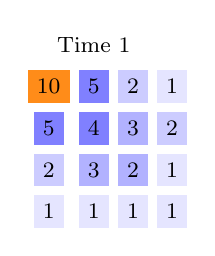
\begin{tikzpicture}[>=latex']
	\tikzset{block/.style= { rectangle, align=left,minimum width=.2cm,minimum height=.1cm},
		rblock/.style={draw, shape=rectangle,rounded corners=1.5em,align=center,minimum width=.2cm,minimum height=.1cm},
		input/.style={ % requires library shapes.geometric
			draw,
			trapezium,
			trapezium left angle=60,
			trapezium right angle=120,
			minimum width=2cm,
			align=center,
			minimum height=1cm
		},
	}
	\node [block, fill=orange!90]  (x1) {\footnotesize 10};
	\node [block, right = .1cm of x1, fill=blue!50] (x2) {\footnotesize 5};
	\node [block, right = .1cm of x2,fill=blue!20] (x3) {\footnotesize 2};
	\node [block, right = .1cm of x3, fill=blue!10] (x4) {\footnotesize 1};
	\node [block, below = .1cm of x1, fill=blue!50] (y1) {\footnotesize 5};
	\node [block, below = .1cm of x2, fill=blue!50] (y2) {\footnotesize 4};
	\node [block, below = .1cm of x3, fill=blue!30] (y3) {\footnotesize 3};
	\node [block, below = .1cm of x4,fill=blue!20] (y4) {\footnotesize 2};
	\node [block, below = .1cm of y1,fill=blue!20] (z1) {\footnotesize 2};
	\node [block, below = .1cm of y2, fill=blue!30] (z2) {\footnotesize 3};
	\node [block, below = .1cm of y3, fill=blue!30] (z3) {\footnotesize 2};
	\node [block, below = .1cm of y4, fill=blue!10] (z4) {\footnotesize 1};
	\node [block, below = .1cm of z1, fill=blue!10] (q1) {\footnotesize 1};
	\node [block, below = .1cm of z2, fill=blue!10] (q2) {\footnotesize 1};
	\node [block, below = .1cm of z3, fill=blue!10] (q3) {\footnotesize 1};
	\node [block, below = .1cm of z4, fill=blue!10] (q4) {\footnotesize 1};
	\node [block, above = .1cm of x2] {\footnotesize Time 1};
	\end{tikzpicture}
	\quad
	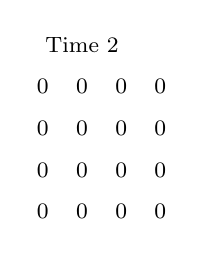
\begin{tikzpicture}[>=latex']
	\tikzset{block/.style= { rectangle, align=left,minimum width=.2cm,minimum height=.1cm},
		rblock/.style={draw, shape=rectangle,rounded corners=1.5em,align=center,minimum width=.2cm,minimum height=.1cm},
		input/.style={ % requires library shapes.geometric
			draw,
			trapezium,
			trapezium left angle=60,
			trapezium right angle=120,
			minimum width=2cm,
			align=center,
			minimum height=1cm
		},
	}
	\node [block]  (x1) {\footnotesize 0};
	\node [block, right = .1cm of x1] (x2) {\footnotesize 0};
	\node [block, right = .1cm of x2] (x3) {\footnotesize 0};
	\node [block, right = .1cm of x3] (x4) {\footnotesize 0};
	\node [block, below = .1cm of x1] (y1) {\footnotesize 0};
	\node [block, below = .1cm of x2] (y2) {\footnotesize 0};
	\node [block, below = .1cm of x3] (y3) {\footnotesize 0};
	\node [block, below = .1cm of x4] (y4) {\footnotesize 0};
	\node [block, below = .1cm of y1] (z1) {\footnotesize 0};
	\node [block, below = .1cm of y2] (z2) {\footnotesize 0};
	\node [block, below = .1cm of y3] (z3) {\footnotesize 0};
	\node [block, below = .1cm of y4] (z4) {\footnotesize 0};
	\node [block, below = .1cm of z1] (q1) {\footnotesize 0};
	\node [block, below = .1cm of z2] (q2) {\footnotesize 0};
	\node [block, below = .1cm of z3] (q3) {\footnotesize 0};
	\node [block, below = .1cm of z4] (q4) {\footnotesize 0};
	\node [block, above = .1cm of x2] {\footnotesize Time 2};
	\end{tikzpicture}
\end{center}
\begin{center}
	Reaction Diffusion Latent Process Conditional on $(s_1,1)=10$
\end{center}
\quad
\begin{center}
	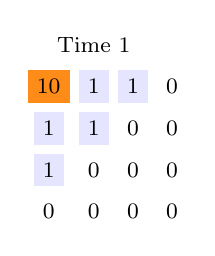
\begin{tikzpicture}[>=latex']
	\tikzset{block/.style= { rectangle, align=left,minimum width=.2cm,minimum height=.1cm},
		rblock/.style={draw, shape=rectangle,rounded corners=1.5em,align=center,minimum width=.2cm,minimum height=.1cm},
		input/.style={ % requires library shapes.geometric
			draw,
			trapezium,
			trapezium left angle=60,
			trapezium right angle=120,
			minimum width=2cm,
			align=center,
			minimum height=1cm
		},
	}
	\node [block, fill=orange!90]  (x1) {\footnotesize 10};
	\node [block, right = .1cm of x1,fill=blue!10] (x2) {\footnotesize 1};
	\node [block, right = .1cm of x2, fill=blue!10] (x3) {\footnotesize 1};
	\node [block, right = .1cm of x3] (x4) {\footnotesize 0};
	\node [block, below = .1cm of x1,fill=blue!10] (y1) {\footnotesize 1};
	\node [block, below = .1cm of x2, fill=blue!10] (y2) {\footnotesize 1};
	\node [block, below = .1cm of x3] (y3) {\footnotesize 0};
	\node [block, below = .1cm of x4] (y4) {\footnotesize 0};
	\node [block, below = .1cm of y1, fill=blue!10] (z1) {\footnotesize 1};
	\node [block, below = .1cm of y2] (z2) {\footnotesize 0};
	\node [block, below = .1cm of y3] (z3) {\footnotesize 0};
	\node [block, below = .1cm of y4] (z4) {\footnotesize 0};
	\node [block, below = .1cm of z1] (q1) {\footnotesize 0};
	\node [block, below = .1cm of z2] (q2) {\footnotesize 0};
	\node [block, below = .1cm of z3] (q3) {\footnotesize 0};
	\node [block, below = .1cm of z4] (q4) {\footnotesize 0};
	\node [block, above = .1cm of x2] {\footnotesize Time 1};
	\end{tikzpicture}
	\qquad
	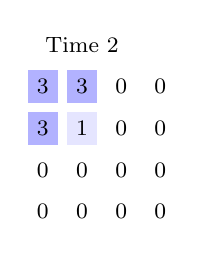
\begin{tikzpicture}[>=latex']
	\tikzset{block/.style= { rectangle, align=left,minimum width=.2cm,minimum height=.1cm},
		rblock/.style={draw, shape=rectangle,rounded corners=1.5em,align=center,minimum width=.2cm,minimum height=.1cm},
		input/.style={ % requires library shapes.geometric
			draw,
			trapezium,
			trapezium left angle=60,
			trapezium right angle=120,
			minimum width=2cm,
			align=center,
			minimum height=1cm
		},
	}
	\node [block,fill=blue!30]  (x1) {\footnotesize 3};
	\node [block, right = .1cm of x1, fill=blue!30] (x2) {\footnotesize 3};
	\node [block, right = .1cm of x2] (x3) {\footnotesize 0};
	\node [block, right = .1cm of x3] (x4) {\footnotesize 0};
	\node [block, below = .1cm of x1, fill=blue!30] (y1) {\footnotesize 3};
	\node [block, below = .1cm of x2, fill=blue!10] (y2) {\footnotesize 1};
	\node [block, below = .1cm of x3] (y3) {\footnotesize 0};
	\node [block, below = .1cm of x4] (y4) {\footnotesize 0};
	\node [block, below = .1cm of y1] (z1) {\footnotesize 0};
	\node [block, below = .1cm of y2] (z2) {\footnotesize 0};
	\node [block, below = .1cm of y3] (z3) {\footnotesize 0};
	\node [block, below = .1cm of y4] (z4) {\footnotesize 0};
	\node [block, below = .1cm of z1] (q1) {\footnotesize 0};
	\node [block, below = .1cm of z2] (q2) {\footnotesize 0};
	\node [block, below = .1cm of z3] (q3) {\footnotesize 0};
	\node [block, below = .1cm of z4] (q4) {\footnotesize 0};
	\node [block, above = .1cm of x2] {\footnotesize Time 2};
	\end{tikzpicture}
	\qquad
	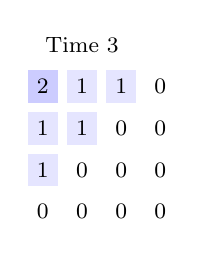
\begin{tikzpicture}[>=latex']
	\tikzset{block/.style= { rectangle, align=center,minimum width=.2cm,minimum height=.1cm},
		rblock/.style={draw, shape=rectangle,rounded corners=1.5em,align=center,minimum width=.2cm,minimum height=.1cm},
		input/.style={ % requires library shapes.geometric
			draw,
			trapezium,
			trapezium left angle=60,
			trapezium right angle=120,
			minimum width=2cm,
			align=center,
			minimum height=1cm
		},
	}
	
	\node [block, fill=blue!20]  (x1) {\footnotesize 2};
	\node [block, right = .1cm of x1, fill=blue!10] (x2) {\footnotesize 1};
	\node [block, right = .1cm of x2, fill=blue!10] (x3) {\footnotesize 1};
	\node [block, right = .1cm of x3] (x4) {\footnotesize 0};
	\node [block, below = .1cm of x1, fill=blue!10] (y1) {\footnotesize 1};
	\node [block, below = .1cm of x2, fill=blue!10] (y2) {\footnotesize 1};
	\node [block, below = .1cm of x3] (y3) {\footnotesize 0};
	\node [block, below = .1cm of x4] (y4) {\footnotesize 0};
	\node [block, below = .1cm of y1, fill=blue!10] (z1) {\footnotesize 1};
	\node [block, below = .1cm of y2] (z2) {\footnotesize 0};
	\node [block, below = .1cm of y3] (z3) {\footnotesize 0};
	\node [block, below = .1cm of y4] (z4) {\footnotesize 0};
	\node [block, below = .1cm of z1] (q1) {\footnotesize 0};
	\node [block, below = .1cm of z2] (q2) {\footnotesize 0};
	\node [block, below = .1cm of z3] (q3) {\footnotesize 0};
	\node [block, below = .1cm of z4] (q4) {\footnotesize 0};
	\node [block, above = .1cm of x2] {\footnotesize Time 3};
	\end{tikzpicture}\\
\end{center}





Practically, if data follows the RDSE model, it implies a high terrorism count in one region will manifest into a high terrorism count in a neighboring region at a later time period.  In combating terrorism, the RDSE might suggest isolating geographical regions to mitigate the risk of spread while addressing self-excitation through direct action against malicious actors who are inspiring others.

\section{Model Fitting}
In both the RDSE and the SCSE, spatio-temporal diffusion exists in both the process model and the data model.  If the diffusion was solely in the process model, a technique for inference would be Integrated Nested Laplace Approximation, or INLA.

INLA was first proposed in \cite{rue2009approximate} to specifically address the issue of Bayesian Inference of high dimensional Latent Gaussian Random Fields, LGRFs.  An example of this for count data is:
\begin{align}
Y(s_i)&\sim \mbox{Pois}(\mu(s_i,t)) \label{eq:model}\\
\mu(\boldsymbol{s_i,t})&=\exp(\lambda(\boldsymbol{s_i},t))\nonumber\\
\lambda(\boldsymbol{s_i},t) &= \beta_0 + \boldsymbol{Z}^t \boldsymbol{\beta} + X(\boldsymbol{s_i,t})\nonumber\\
\boldsymbol{X}& \sim \mbox{Gau}(\boldsymbol{0},Q^{-1}(\theta))\nonumber	
\end{align}

INLA is often preferable over MCMC for these types of models.  An issue with traditional Markov Chain Monte Carlo (MCMC) techniques for these models is that the dimension of $X$ is often very large.  Therefore, while MCMC has $O_p(N^{-1/2})$ errors, the $N$ in the errors is the simulated sample size for the posterior.  Just getting $N=1$ may be extremely difficult due to the vast number of elements of $X$ that need to be estimated.  In general, MCMC will take hours or days in order to successfully simulate from the posterior making the computational cost of fitting multiple process models extremely high.  In \cite{python2016bayesian}, terrorism data was fit using a grid over the entire planet using INLA, though without self-excitation in the model.

To address the issues with MCMC use in LGRFs, \cite{rue2009approximate} developed a deterministic approach based on multiple Laplacian approximations. A LGRF is any density that can be expressed as
\begin{equation}
\pi(\boldsymbol{\theta},\boldsymbol{X} |\boldsymbol{Y}) \propto \pi (\theta)|Q(\boldsymbol{\theta})|^{1/2}\exp \left[\frac{-1}{2}\boldsymbol{X}^t Q(\boldsymbol{\theta}) \boldsymbol{X}+\sum_{\boldsymbol{s}} \log\left(\pi(Y(\boldsymbol{s_i})|X(\boldsymbol{s_i}),\boldsymbol{\theta})\right)\right]
\end{equation} 
In order to conduct inference on this model, we need to estimate $\pi(\boldsymbol{\theta}|\boldsymbol{y})$, $\pi(\theta_i|\boldsymbol{y})$ and $\pi(x_i|\boldsymbol{y})$.  The main tool \cite{rue2009approximate} employ is given in their equation (3) as
\begin{equation}
\tilde{\pi}(\boldsymbol{\theta}|\boldsymbol{Y})\propto \frac{\pi(\boldsymbol{X},\boldsymbol{\theta},\boldsymbol{Y})}{\tilde{\pi}_G (\boldsymbol{X}|\boldsymbol{\theta},\boldsymbol{Y})}|_{X=x^*(\boldsymbol{\theta})}\label{eq:main}
\end{equation}

In \cite{rue2009approximate} they note that the denominator of \eqref{eq:main} almost always appears to be unimodal and approximately Gaussian.  The authors then propose to use a Gaussian approximation to $\pi(\boldsymbol{X}|\boldsymbol{\theta},\boldsymbol{Y})$ which is denoted above as $\tilde{\pi}_G$.  Moreover, \eqref{eq:main} should hold no matter what choice of $\boldsymbol{X}$ is used, so a convenient choice for $\boldsymbol{X}$ is the mode for a given $\theta$, which \cite{rue2009approximate} denote as $x^*(\boldsymbol{\theta})$.  

Now, $\pi(\boldsymbol{\theta}|\boldsymbol{Y})$ can be explored by calculating the marginal for choices of $\theta$, which if chosen carefully can greatly decrease the computational time.  These explored values can then be numerically integrated out to get credible intervals for $\pi(\theta_i|\boldsymbol{Y})$.

Following the exploration of $\theta|Y$, and computation of $\theta_i|Y$, INLA next proceeds to approximate $\pi(X(s_i)|\boldsymbol{\theta},\boldsymbol{Y})$.  The easiest way to accomplish this is to use the marginals that can be derived straightforwardly from $\tilde{\pi}_G(\boldsymbol{X}|\boldsymbol{\theta},\boldsymbol{Y})$ from \eqref{eq:main}.  In this manuscript we will use this technique for simplicity of computation, however, if the latent states are of interest in the problem (and they often are), this can be problematic as it fails to capture any skewness of the posterior of $\boldsymbol{X}$.  One way to correct this is to re-apply \eqref{eq:main} in the following manner:
\begin{equation}
\tilde{\pi}_{LA}(X(\boldsymbol{s_i})|\theta,y)\propto \frac{\pi(\boldsymbol{X},\theta,\boldsymbol{Y})}{\tilde{\pi}_G(\boldsymbol{X}_{-s_i}|X(s_i),\boldsymbol{\theta},\boldsymbol{Y})}|_{x_{-i}=\boldsymbol{x_{-i}}^*(x_i,\theta)}\label{eq:remain}
\end{equation}
In \eqref{eq:remain} $\boldsymbol{X}_{-s_i}$ is used to represent $\boldsymbol{X}$ with latent variable $X(s_i)$ removed.  This is a reapplication of Tierney and Kadane's marginal posterior density and gives rise to the nested term in INLA. 

\subsection{Laplace Approximation for Spatio-Temporal Self-Exciting Models}
While INLA is an attractive technique due to computational speed and implementation, it is not immediately usable for the SCSE and the RDSE as the structure in \eqref{eq:gen Model} is
\begin{align}
\mu(\boldsymbol{s_i},t) & = \exp(X(\boldsymbol{s_i},t)) + \eta Y(\boldsymbol{s_i},t-1)\nonumber\\
& \eta \in (0,1)
\end{align}
In this structure, $X(.)$ and $Y(.)$ are not linearly related and a Gaussian prior for $\eta$ is clearly not appropriate due to the parameter space constraints.


However, Laplace approximations can still be used by conducting inference on $\eta$ at the same time inference is conducted on the the set of latent model parameters.  In both the Spatially Correlated Self-Exciting Model and the Reaction Diffusion Self-Exciting model, the full conditional for the latent state is
\begin{equation}
\footnotesize\pi(\boldsymbol{X}|\boldsymbol{Y},\boldsymbol{\theta}) \propto \exp\left(-\frac{1}{2}\boldsymbol{X}^T \boldsymbol{Q(\boldsymbol{\theta})}\boldsymbol{X} + \sum_{s_i,t} \log \pi\left(Y(\boldsymbol{s_i},t)|X(\boldsymbol{s_i},t),\eta,Y(\boldsymbol{s_i},t-1)\right)\right)\label{eq:FullCond}
\end{equation} 
Here we will let $\boldsymbol{\theta}=(\theta_1,\sigma^2,\eta)^T$ and $\boldsymbol{Q_{sc}(\boldsymbol{\theta})}=(\boldsymbol{I}_{sn,sn}-\theta_1\boldsymbol{I}_{t,t} \otimes \boldsymbol{H})$ for the Spatially Correlated Self-Exciting Model and use $\boldsymbol{Q_{rd}(\boldsymbol{\theta})}$ for the RDSEM defined in \eqref{eq:Prec}.

While $\boldsymbol{\theta}$ in \eqref{eq:FullCond} does not contain $\eta$ we next do a Taylor series expansion of \begin{equation*}\log \pi\left(Y(\boldsymbol{s_i},t)|X(\boldsymbol{s_i},t),\eta,Y(\boldsymbol{s_i},t-1)\right),\end{equation*} as a function of $X(\boldsymbol{s_i},t)$ and, for each $\boldsymbol{s_i},t$, expand the term about a guess for the mode, say $\mu_0(\boldsymbol{s_i},t)$.  First we write $\boldsymbol{B^*}(\boldsymbol{\theta}|\mu_0)$ as a vector of the same length as $X(\boldsymbol{s_i},t)$ where each element is given by
\begin{equation}
B(\boldsymbol{s_i},t|\mu_0)=\left(\frac{\partial \log\pi\left(Y(\boldsymbol{s_i},t)\right)}{\partial X(\boldsymbol{s_i},t)}\Bigr|_{X(\boldsymbol{s_i},t)=\mu(\boldsymbol{s_i},t)}-\mu(\boldsymbol{s_i},t) \frac{\partial^2\log\pi\left(Y(\boldsymbol{s_i},t)\right)}{\partial X(\boldsymbol{s_i},t)^2}\Bigr|_{X(\boldsymbol{s_i},t)=\mu(\boldsymbol{s_i},t)}\right)\label{eq:B(si)}
\end{equation}

Next, we further define
$\boldsymbol{Q^*(\boldsymbol{\theta})}|\mu_0$ as the updated precision matrix.
\begin{equation}
\boldsymbol{Q^*(\boldsymbol{\theta})|\mu_0}=\boldsymbol{Q(\boldsymbol{\theta})}+\text{diag }\left(-\frac{\partial^2\log \pi\left(Y(\boldsymbol{s_i},t)\right)}{\partial X(\boldsymbol{s_i},t)^2}\right)\Bigr|_{X(\boldsymbol{s_i},t)=\mu(\boldsymbol{s_i},t)} \label{eq:Precision at Mode}\\
\end{equation}
Where $\boldsymbol{Q(\boldsymbol{\theta})}$ is either $\boldsymbol{Q_{sc}(\boldsymbol{\theta})}$ or $\boldsymbol{Q_{rd}(\boldsymbol{\theta})}$ depending on the context.  Then we can write
\begin{equation}
\footnotesize\pi(\boldsymbol{X}|\boldsymbol{Y},\boldsymbol{\theta}) \propto \exp\left(-\frac{1}{2}\boldsymbol{X}^T\left( \boldsymbol{Q^*(\boldsymbol{\theta})|\mu_0}\right)\boldsymbol{X} + \boldsymbol{X}^T\left( \boldsymbol{B^*}(\boldsymbol{\theta})|\boldsymbol{\mu_0}\right)\right) \label{eq:FullCondExpand}
\end{equation}


While in \eqref{eq:Precision at Mode}, $\boldsymbol{Q}(\boldsymbol{\theta})$, the original precision matrix, does not contain $\eta$, $\boldsymbol{Q^*(\boldsymbol{\theta})}$, the updated precision matrix, does depend on the self-excitation parameter.


Next we find the values of $\mu(\boldsymbol{s_i})$ that maximize \eqref{eq:FullCondExpand}.  This is done through the use of an iterative maximization algorithm by solving for $\boldsymbol{\mu_1}$ in $\left(Q^*(\boldsymbol{\theta})|\boldsymbol{\mu_0}\right)\boldsymbol{\mu_1}=\boldsymbol{B^*}(\boldsymbol{\theta}|\mu_0)$. For a fixed $\boldsymbol{\theta}$, this converges rapidly, due to the sparsity of both $\boldsymbol{Q_{sc}}$ and $\boldsymbol{Q_{rd}}$.  .

In \eqref{eq:main}, for a fixed $\boldsymbol{\theta}$, we can then find $x^*(\boldsymbol{\theta})$.  When the denominator of \eqref{eq:main} is evaluated at $x^*(\boldsymbol{\theta})$ it becomes $|\boldsymbol{Q^*(\boldsymbol{\theta})}\frac{1}{2\pi}|^{1/2}$ which is equivalent to the hyperparameter inference recommended by \cite{lee1996hierarchical} as pointed out by R. A. Rigby in \cite{rue2009approximate}.  

In order to best explore $\pi(\boldsymbol{\theta}|\boldsymbol{Y})$ the posterior mode is first found through a Newton-Raphson based method.  In order to do this we approximate the Hessian matrix based off of finite difference approximation to the second derivatives.  


After locating the posterior mode of $\pi(\boldsymbol{\theta}|\boldsymbol{Y})$, the parameter space can be explored using the exploration strategy laid out in section 3.1 of \cite{rue2009approximate}.

Now, for the set of diffusion parameters, $\boldsymbol{\theta}$ which contain $\eta$, we have a method of estimating $\pi(\boldsymbol{\theta}|\boldsymbol{Y})$.  Inference for any further data model covariates can now be conducted in the same manner as done in \cite{rue2009approximate}. 
\subsection{Model Comparison and Goodness of Fit}
In order to conduct model comparison, we will use the deviance information criterion (DIC) originally proposed by \cite{spiegelhalter2002bayesian}.  Goodness of fit will be conducted through the use of posterior predictive p-values, outlined by \cite{gelman1996posterior}.

To approximate the DIC, we first find the effective number of parameters for a given $\boldsymbol{\theta}$.  As noted in \cite{rue2009approximate}, we can estimate this by using $n-\text{tr}\left(\boldsymbol{Q(\theta)}\boldsymbol{Q^*(\theta)}^{-1}\right)$ for both the SCSEM and the RDSEM.  This gives the effective number parameters for a given $\boldsymbol{\theta}$, which can then be averaged over $\pi(\boldsymbol{\theta}|\boldsymbol{Y})$ to get the effective number of parameters for the model.

Secondly, we calculate the deviance of the mean
\begin{equation}
-2\sum_{s_i,t} \log \pi\left(Y(s_i,t)|\hat{X}(s_i,t),\boldsymbol{\theta^*}\right)
\end{equation} where $\boldsymbol{\theta^*}$ is the posterior mode and $\hat{X}(s_i,t)$ is the expectation of the latent state fixing $\theta=\theta^*$.  DIC can then be found through deviance of the mean plus two times the effective number of parameters as in chapter 7 of \cite{gelman2014bayesian} and initially recommended by \cite{spiegelhalter2002bayesian}.

In order to assess goodness of fit in analyzing the terrorism data in Section 5, we will use posterior predictive P-values as described by \cite{gelman1996posterior}.  Here, we pick critical components of the original dataset that we wish to see if the fitted model can accurately replicate, for instance the number of zeros in the dataset which we can designate as $T(\boldsymbol{Y})$.  Next, for an index $m=1...M$, We then draw a value of $\boldsymbol{\theta_m}$ according to $\pi(\boldsymbol{\theta}|\boldsymbol{Y})$ and simulate a set of observations $Y^*(\boldsymbol{s_i,t})_m$ of the same dimension as $\boldsymbol{Y}$ and compute $T(\boldsymbol{Y}^*_m)$.  This process is repeated M times and a posterior predictive p-value is computed as $\frac{1}{M}\sum_{m=1}^M I\left[T(\boldsymbol{Y}^*_m) > T(\boldsymbol{Y}) \right]$ where $I\left[ . \right]$ is the indicator function.  While not a true P-value, both high and low values of the posterior predictive p-value should cause concern over the fitted models ability to replicate features of the original dataset.

\section{Simulation}

In order to validate the Laplace based methodology for spatially correlated self-exciting models we conducted simulation studies using data on a 8 by 8 Spatial grid assuming a rook neighborhood structure.  In order to decrease the edge effect, we wrapped the grid on a torus so each node had four neighbors.  For each grid location we simulated 100 observations, creating a spatio-temporal model that had 6400 observations, meaning in \eqref{eq:main}, $\boldsymbol{Q}(\boldsymbol{\theta})$ had a dimension of $6400 \times 6400$.

In the first simulation we used \eqref{eq:Full Model} fixing the parameters at values that generated data that appeared to resemble the data from Iraq used in Section 5.  The generating model we used was:

\begin{align}
& Y(\boldsymbol{s_i},t)|\mu(\boldsymbol{s_i},t) \sim \text{Pois }(\mu(\boldsymbol{s_i},t)) \label{eq:First Simulation}\\
& \mu(\boldsymbol{s_i},t) = \exp(-1+X(\boldsymbol{s_i},t)) + .2 Y(\boldsymbol{s_i},t-1) \nonumber \\
& X(\boldsymbol{s_i},t) = .22 \sum_{\boldsymbol{s_j}\in N(\boldsymbol{s_i})}X(\boldsymbol{s_j},t) + \epsilon(\boldsymbol{s_i},t) \nonumber\\
&\epsilon(\boldsymbol{s_i},t) \sim Gau(0,.4) \nonumber
\end{align}

The spatial parameter for model was $\theta_1=.22$ which suggests a positive correlation between spatially adjacent locations.  An $\eta$ value of 0.2 would suggest that each event that occurs at one time period increases the expected number of events at the next time period by .2.  Here we fix $\sigma^2$ was fixed at 0.4 and use a value of $\beta_0=-1$  to reflect that in real world applications the latent process likely is not zero mean.

Once the data were generated, we found $\pi(\boldsymbol{\theta}|\boldsymbol{Y})$ by applying \eqref{eq:main}.  Here we note that the numerator of \eqref{eq:main} is $\small\pi(\boldsymbol{X},\boldsymbol{\theta},\boldsymbol{Y})=\pi(\boldsymbol{Y}|\boldsymbol{X},\eta,\boldsymbol{\theta})\pi(\eta)\pi(\boldsymbol{X}|\theta_1,\sigma^2)\pi(\theta_1)\pi(\sigma^2)$ which requires a prior specification for $\eta$,$\theta_1$, and $\sigma$.  In order to reflect an a-priori lack of knowledge we choose vague priors for all parameters.   In this model, we use a Half-Cauchy with scale parameter of 25 for $\sigma$ and a Uniform ($\psi_{1}^{-1},\psi_{n}^{-1}$) where $\psi_(i)$ is the $i$th largest eigen vector of the spatial neighborhood.  As we used a shared-boreder, or rook, neighbor structure wrapped on a torus, the parameter space is (-0.25,.025) as each spatial location has four neighbors.  The choice of the Half-Cauchy is in line with the recommendations for vague priors for variance components of hierarchical models as outlined in \cite{gelman2006prior} and rigorously defended in \cite{polson2012half}.  We let the prior for $\eta$ be Uniform(0,1).  

Using a gradient descent method with step-halving we found the posterior mode of $\pi(\boldsymbol{\theta}|\boldsymbol{Y})$ to be $\sigma^2=0.32$, $\theta_1=0.22$, and $\eta=0.20$. Using the z based parameterization described in Section 3.1 we next explored the parameterization $\log\pi(\boldsymbol{\theta}|\boldsymbol{Y})$ and found credible intervals of $\pi(\sigma^2|\boldsymbol{Y})=(0.29,0.36),\pi(\theta_1|\boldsymbol{Y})=(0.22,0.23)$ and $\pi(\eta|\boldsymbol{Y})=(.18,.21)$.  Fixing $\boldsymbol{\theta}$ at the posterior mode, we then found an approximate 95\% credible interval for $\beta_0$ to be (.07,-1.67).  If further refinement for $\beta_0$ was required, we could proceed to use \eqref{eq:remain}.  This was not done here as $\beta_0$ was not the subject of our primary inference.

The posterior maximum and credible interval for $\sigma^2$ appear to be slightly lower than expected, but the remaining parameter credible intervals covered the generating parameter.  

Next we simulated from the reaction-diffusion self-excitation model letting $\beta_0=0$, $\alpha=0.1$, $\kappa=0.2$, $\sigma^2=0.25$, and $\eta=0.4$ 

In fitting the model, we again use vague priors for all the parameters.  Again, we place a Half-Cauchy prior on $\sigma^2$ as described above.  In order to conform to the parameter space of $\alpha$ and $\kappa,$ we let $\pi(\alpha)\sim \text{Unif }(0,1)$ and $\pi(\kappa|\alpha)\sim\text{Unif }(-\frac{\alpha}{2},1-\frac{\alpha}{2})$.


Again using the Laplace approximation technique of section 3, we found the posterior mode of $\pi(\boldsymbol{\theta}|\boldsymbol{Y})$ to be at $\alpha=0.085$, $\kappa=0.19$, $\sigma^2=0.21$, $\eta=0.35$.  95\% credible intervals for the posterior marginals were $\alpha \in (0.07, 0.10)$, $\kappa \in (0.14,0.24)$, $\sigma^2 \in (0.18,0.24)$, and $\eta \in (0.32, 0.40)$.  At the posterior mode of $\boldsymbol{\theta}$, the  posterior marginal for $\beta_0$ was approximately (-0.03,0.01).  Critically, if there is self-excitement in the data, in all simulations it was differentiable from the latent diffusion.  This is a spatial-temporal analogue to the finding in \cite{mohler2013modeling} where a temporal AR(1) process was differentiable from self-excitement.


In our simulations, the approximations described in this manuscript performed reasonably well for inference on the spatio-temporal diffusion parameters in most cases.  However, when $\sigma^2$ is large, or when $\eta$ is large, we have found that the approximations create bias in one or more of the parameters likely due to the high effective number of parameters.  However, all approximate likelihood based methods will likely struggle in these cases as well.  As noted in \cite{rue2009approximate}, the approximation error in Laplace based methods is related to the number of effective latent variables over the total sample size.


\section{Spatio-Temporal Diffusion of Violence in Iraq (2003-2010)}

\subsection{Statistical Models and Data}

One region where the reasons for the diffusion of terror and crime still remains unclear is in Iraq during 2003 to 2010.  While violence undoubtedly spread throughout the country, it remains unclear how or why, spatio-temporally, the spread occurred.  Part of the uncertainty is that there still is not agreement over whether violence was due to insurgency, civil war, or organized crime. For example, \cite{hoffman2006insurgency} refers to the violence in Iraq as an insurgency, \cite{fearon2007iraq} argues that the spread of violence was due to a civil war, and \cite{williams2009criminals} argues that there was a large presence of organized crime in the country.  

A few previous studies have examined the presence or absence of self-excitaiton.  In \cite{lewis2012self}, the authors concluded that self-excitation was present in select cities in Iraq during this time period.  The presence of the self-excitation finding was echoed in \cite{braithwaite2015battle} where the authors also noted a correlation between locations that shared microscale infrastructure similarities.  This would suggest repeat or near-repeat actions were causing the increase in violence in a region.

However, in both of these cases, the latent spatio-temporal diffusion was, a-priori, assumed to be known.  In fact, this is likely not the case. In a classic work on the subject, \cite{midlarsky1980violence} discuss how heterogeneity between locations can cause correlation in violence or individuals who cause violence can actually physically move from one location to another.  In particular, if violence is strictly due to crime we would expect self-excitement and limited diffusion between geographical regions.  Whereas if violence is due to insurgencies we would expect more movement of actors as they seek to create widespread disruption in the country.
The former theory is reflected in the Spatial Correlation in the Spatially Correlated Self-Exciting model and the later theory would correspond to the Reaction Diffusion component of the second model.  

The overarching goal of this analysis, thus, is to determine whether in Iraq the growth of violence in fixed locations was due to the presence or absence of self-excitation.  Furthermore, we want to determine whether the latent diffusion of violence is due to the movement of population such as in the Reaction Diffusion model, or whether there is static spatial correlation.  We will answer this while controlling for exogenous factors that may also explain the rise in violence in a region.


In order to address this question as well as demonstrate how Laplace based approximations can be used to fit real world data to models of the class of \eqref{eq:model} we used data from the Global Terrorism Database (GTD) introduced in \cite{lafree2007introducing} to examine the competing theories.  The GTD defines terrorist events as events that are intentional, entail violence, and are perpetrated by sub-national actors.  Additionally, the event must be aimed at obtaining a political, social, religions, or economic goal and must be conducted in order to coerce or intimidate a larger actor outside of the victim.  The majority of lethal events in Iraq from 2003-2010 fit the above category.

The GTD uses a variety of open media sources to capture both spatial and temporal data on terroristic events.  The database contains information on what the event was, where it took place, when it took place, and what terrorist group was responsible for the event.  From 2003 to 2010 in Iraq, the database contains 6263 terrorist events, the spatial structure is shown in figure \ref{SpaceIZ}.  

\begin{figure}[h] % figuur 1
	\begin{center}
		\vspace{6pc}
		\includegraphics[width=.8 \linewidth]{IncidentsOverPop.pdf}
		\isucaption[Location of Violent Events in Iraq]{Spatial depiction of 6263 events in Iraq.}
		\label{SpaceIZ}
	\end{center}
\end{figure} 

As seen in this map, the majority of the violence is in heavily populated areas such as Baghdad and in the regions north up the Tigris river to Mosul and west through the Euphrates river.  In order to model this data, we aggregated the point data to 155 political districts intersected by ethnicities and aggregated the data monthly for 96 months meaning that $\Sigma(\theta)$ in \eqref{eq:gen Model} is a 14880 x 14880 matrix.  Population for each political district was taken from the Empirical Studies of Conflict Project website, available from https://esoc.princeton.edu/files/ethnicity-study-ethnic-composition-district-level.  

We considered covariates controlling for the population density within a fixed region as well as for the underlying ethnicity.  We will make the simplifying assumption that both of these are static over time.  Previous statistical analysis on terrorism considered macro level covariates, such as democracy in \cite{python2016bayesian} that differ country to country but would not change within a single country as analyzed here.  Other studies considered more micro level covariates such as road networks that were found to be statistically related to terrorism in \cite{braithwaite2015battle}.  Here we take the view point that the vast majority of the incidents in Iraq were directed against individuals rather than terrorist events directed at fixed locations.  Therefore, we would expect a higher population density to provide more targets for a potential terrorist to attack.  Furthermore, covariates such as road networks, number of police, or number of US soldiers, would all be highly collinear with population density.  We do, though, consider a covariate for ethnicity in a region.  Specifically, we add an indicator if the region is predominately Sunni.    The disenfranchisement of the Sunnis and high level of violence in Sunni dominated areas has been well established, see for e.g. \cite{baker2006iraq}.  Previous research in \cite{linke2012space} focusing on Granger Causality also suggested indicators for majority Sunni/Shia may be appropriate in any analysis of violence in Iraq.


\begin{align}
& Y(\boldsymbol{s_i},t)|\mu(\boldsymbol{s_i},t) \sim \text{Pois }(\mu(\boldsymbol{s_i},t)) \label{eq:IZ Model}\\
& \mu(\boldsymbol{s_i},t) = \exp[\beta_0+\beta_1\log \text{Pop}(\boldsymbol{s_i})+\beta_2\text{Sunni }(\boldsymbol{s_i})+X(\boldsymbol{s_i},t)] + \eta Y(\boldsymbol{s_i},t-1) \nonumber \\
& \boldsymbol{X}\sim \mbox{Gaus}(\boldsymbol{0},\boldsymbol{Q}^{-1}(\theta))  \nonumber
\end{align}

The complete statistical model is given in \eqref{eq:IZ Model}.  We next fit this model letting $\boldsymbol{Q}=\boldsymbol{Q_{sc}}$ and $\boldsymbol{Q}=\boldsymbol{Q_{rd}}$.  We further consider fixing $\eta=0$ to test the presence or absence of self-excitement in the data for both process models.


\subsection{Results}



We fit all four models using the Laplace approximation method described in Section 3.1.  For each of the parameters we used vague proper priors to ensure posterior validity.  In the SCSEM and the Spatially Correlated models we used a Half-Cauchy with scale parameter of 5 for $\sigma$ and a Uniform ($\psi_{1}^{-1},\psi_{n}^{-1}$) where $\psi$ are the eigenvalues of $\boldsymbol{H}$.  Using the neighborhood structure corresponding to the geographical regions described above, this corresponded to a Uniform (-.3,.13). For each of the exogenous covariates, we used independent Gaussian (0,1000) priors.  For the SCSEM model we further assumed a Uniform (0,1) prior for $\eta$.

In fitting the RDSEM, we again used a Half-Cauchy with scale parameter of 5 for $\sigma$.  For the decay parameter, $\alpha$, we used a Uniform (0,1) prior and for the diffusion parameter, $\kappa$, we chose a Uniform $\left(\frac{-\alpha}{2},1-\frac{\alpha}{2}\right)$ in order to ensure we were in the allowable parameter space.



\begin{table}[h]
	\caption {95\% Credible Intervals for Model Parameters} \label{tab:params} 
	\begin{center}
		\begin{tabular}{ |c|c|c|c|c| } 
			\hline
			& Spatial Correlation Only & SCSEM & Reation Diffusion Only & RDSEM \\
			\hline 
			$\beta_0$&(-20.2,-18.4) &(-16, -15.5) &(-22.4,-18.0) &(-22,-18.6 )\\
			$\beta_1$& (1.2,1.4)&(0.9, 1.1) &(1.1, 1.4) &(1.1, 1.5)\\
			$\beta_2$& (1.6,1.9)&(1.1,1.3) &(0.10, 0.33) &(0.17, 0.53)\\
			$\eta$& - &(0.35,0.37) & -  &(0, 0.04)\\
			$\sigma^2$&(1.9,2.7) &(2.1, 2.5) & (0.20, 0.30)&(0.18,0.26)\\
			$\theta_1$&(.08,.10) &(0.09,0.1) & - & - \\
			$\alpha$& - & - & (0.001, 0.007) &(0.001, 0.007)\\
			$\kappa$& - & - & (0.03, 0.07) &(0.03, 0.06) \\
			\hline
		\end{tabular}
	\end{center}
\end{table}


All four models took approximately 30 min to an hour depending on starting values to converge using a Newton-Raphson based algorithm to find the maximum.  Gaussian approximations to the 95\% credible intervals for the parameters are given for all four models are shown in table \ref{tab:params}.  As can be seen in comparing the SCSEM to the RDSEM, the presence or absence of self-excitation appears to be dependent on the choice of structure of $\boldsymbol{Q}$.  Furthermore, the impact of majority Sunni is also dependent on whether the Reaction Diffusion or Spatially Correlated model was used.

Using the methodology described in Section 3.2, we next calculated DIC as well as posterior predictive P-values based off of the maximum observed value and the number of zeros in the dataset.  In the original dataset, the maximum number of events observed for all regions and months was 26 and the dataset had 13445 month/district observations that were zero. The model assessment and selection results are shown in Table \ref{tab:results}.
\begin{table}
	\caption {Model Assessment and Selection Statistics For Iraq Data} \label{tab:results} 
	\begin{center}
		\begin{tabular}[H]{|c|c|c|c| } 
			\hline
			Model & DIC & \begin{tabular}{@{}c@{}}P-Values\\ Maximum Value \end{tabular} & \begin{tabular}{@{}c@{}}P-Value \\ Zeros\end{tabular} \\
			
			\hline
			\begin{tabular}{@{}c@{}}Spatially Correlated Model \\ without Self-Excitation \end{tabular} & 9370 & .02 & 1 \\
			\hline	
			\begin{tabular}{@{}c@{}}Spatially Correlated \\ Self-Exciting Model \end{tabular} &  8722 & .97 & 0\\
			\hline 
			\begin{tabular}{@{}c@{}}Reaction Diffusion \\ Only Model \end{tabular} & 8664 & .53 & .81\\
			\hline
			\begin{tabular}{@{}c@{}}Reaction Diffusion \\ Self-Exciting Model \end{tabular} & 8699 & .45 & .89\\
			\hline
		\end{tabular}
	\end{center}
\end{table}

Clearly from table \ref{tab:results}, the models with an underlying reaction diffusion process model outperform those with spatial correlation only.  Furthermore, the addition of self-excitation in the model appears to have minimal impact.  In particular, without self-excitation, the spatial correlation model tends to under count the number of violent activities while the SCSEM tends to over count.  There really is not much difference between the RDSEM and the reaction diffusion model so we prefer the simper reaction diffusion only model. While $\beta_2$ is only minimally significant in the reaction diffusion model, the models perform better including the covariate than disregarding it entirely.

\subsection{Significance}

Under all measures of performance, the reaction diffusion model, \eqref{eq:ReacDiffuse Model}, without self-excitation outperforms the other models under consideration.  This process model as well as values of the covariates and the lack of self-excitement in the data offer several insights into the causes of the spread of violence in Iraq.

Not surprisingly, the reaction diffusion model has a positive relationship between log population and violence.  As the majority of attacks are directed at individuals it would clearly follow that regions that have higher population will offer more targets as well as more potential combatants.  Further, higher populated areas also would have had higher number of Iraqi government officials as well as US military presence.  The positive, though small, relationship between Sunni and violence is also not surprising as, in general, predominately Sunni areas were generally more disenfranchised following the transition to a new Iraqi government after the downfall of Saddam Hussein.

More significantly, though, was that the reaction diffusion model fit the data better than the SCSEM or the RDSEM.  This suggests that increases in violence can be attributed, at least in part, to movement between high violence and low violence areas rather than repeat or near-repeat actors in a fixed location.


While the $\kappa$ parameter may appear small in \ref{tab:params} it still has an impact on the process.  For the sake of simplicity, we can demonstrate this on a three node system.  For this system we consider a central node that has a high level of violence surrounded by two nodes that have a low level of violence. In this set up we will fix $\beta_0=-19$, $\beta_1=1.3$ and consider each node as having a population of 1000 and let $\kappa \in \{.03,.07\}$.  The resultant system over time is shown in Figure \ref{fig:kappa}.   Even in this simple system, there is a noticeable increase in violence as the center node diffuses throughout the entire system.  


\begin{figure}[h]
	\vspace*{.51cm}
	\centering
	\includegraphics[width=8cm]{kappasensitivity}
	\isucaption[Sensitivity of response to change in diffusion parameter]{This plot shows the expected changes in violence in a simple three node system where the center node starts with a high level of violence and the other two nodes start with a low level of violence for $\kappa=.03$, depicted as dashed lines in above figure, and $\kappa=.07$, depicted as straight lines.  As seen here after 12 months for $\kappa=.07$ the nodes are essentially at equilibrium. }
	\label{fig:kappa}
\end{figure}

The implications of the reaction-diffusion model being preferable over the SCSEM or the spatial correlation only model can be seen by going back to the original PDE that inspired the model, \eqref{eq:Reaction}.  The underlying assumption in that model is that violence is that the rate of violence spreading to a region is determined through the levels of violence in neighboring region.  From a military planning perspective, this would suggest that if there is a peaceful region surrounded by areas of high violence, the peaceful region should be isolated to prevent the movement of malicious actors.  This strategy would be consistent with published military strategy as outlined in \cite{army2006counterinsurgency}.


Finally, this offers insight into the nature of the conflict that was fought in Iraq.  For instance, \cite{zhukov2012roads} discuss how insurgencies diffuse throughout a population by either physical movement of actors or through movement of ideas, whereas \cite{short2008statistical} suggest that criminal violence would be expected to have an element of self-excitation.  When accounting for the possibility of spatial diffusion, this self-excitation does not appear to be present in the Iraqi dataset. Therefore, as a diffusion based model fits the data better, this would suggest the spread of violence was due to the physical movement of an insurgent population or ideology rather than a criminal element that would be expected to stay more static at a location.




\section{Discussion}

In this manuscript we develop statistical models that allow for spatio-temporal diffusion in the process model and temporal diffusion in the data model.  We relate the models to existing theory in how violence diffuses in space and time.  We further developed a Laplace approximation for spatio-temporal models that contain self-excitement.  This modification allows for a quick and accurate fit to commonly used models in both the analysis of terrorism and criminology. A critical difference between classical INLA and our proposal is that in our proposal, inference is not only performed on the hyperparameters during the exploration of $\pi(\theta|Y)$ in \eqref{eq:main} but also on the self-excitation parameter $\eta$.  While $\eta$ is not generally thought of as a hyperparameter, when the linear expansion of the log-likelihood is done in \eqref{eq:FullCondExpand}, $\eta$ enters into $\boldsymbol{Q^*}$ and $\boldsymbol{B^*}$ in a similar manner as the hyperparameters. 

While we only considered two process models and self-excitation that only exists for one time period, the methodology outlined above can easily be extended to allow self-excitation to have an exponential decay similar to the modeling technique of \cite{mohler2011self}.  As shown above, the absence of testing multiple process models may result in premature conclusions about how violence is spreading over regions.  While self-excitation may be present in one model, its significance may be dulled through the use of alternative process models resulting in differing conclusions.

Although self-excitation has become increasingly popular, alternate approaches based on Besag's auto-logistic model, as used in \cite{weidmann2010predicting} are possible, though care must be taken if count data is used as Besag's auto-Poisson does not permit positive dependency. As shown in \cite{kaiser1997modeling}, a Winsorized Poisson must be used if positive dependency is desired, as it most certainly is in terrorism modeling.  In this case, the data model dependency would linearly be associated with the log of $\mu(\boldsymbol{s_i},t)$.

Though the motivation for the models in this manuscript was the spatio-temporal spread of violence, the novel concept of combining latent process dependency and data model dependency has the potential to be used in other fields.  For example in the modeling of thunderstorms, self-excitation may be present temporally, while process model dependency may also be appropriate due to small-scale, unobservable, spatial or spatio-temporal dependency.  Laplace approximations, as demonstrated in this manuscript, allow for quick and relatively accurate methods to fit multiple types of self-exciting spatio-temporal models for initial inference. 
\chapter{A Spatially Correlated Auto-Regressive Model For Count Data}\label{JASA}
\begin{center}
	A paper to be submitted to \textit{The Journal of the American Statistical Association}
\end{center}
\section*{Abstract}
	The statistical modeling of multivariate count data observed on a space-time lattice has generally focused on using a hierarchical modeling approach where space-time correlation structure is placed on a continuous, unobservable, process.  The count distribution is then assumed to be conditionally independent given the latent process.  However, in many real-world applications, especially in the modeling of criminal or terrorism data, the conditional independence between the count distributions is inappropriate.  In the absence of spatial correlation, the Integer Auto-Regressive Conditionally Heteroskedastic (INGARCH) process could be used to capture this data model dependence however this model does not allow for any unexplained spatial correlation in the data. In this manuscript we propose a class of models that extends the INGARCH process to account for small scale spatial variation, which we refer to as a SPINGARCH process. The resulting model allows both data model dependence as well as dependence in a latent structure.  We demonstrate how second-order properties can be used to differentiate between models in this class.  Finally, we apply Bayesian inference for the SPINGARCH process demonstrating its use in modeling the spatio-temporal structure of burglaries in Chicago from 2010-2015.


\section{Introduction} 

The modeling of count data where each observation takes place on a space-time lattice arises in multiple disciplines.  In the disease literature, the number of infected patients is often aggregated over geographic areas and discrete times to protect the confidentiality of patients.  In the modeling of terrorism or crime data, data is often presented aggregated over time and space for security reasons.  Even for spatial continuous and temporally continuous data, the analysis is often performed aggregated over fixed spatial and temporal domains as a matter of convenience.  The challenge, then, is how to appropriately model the relationship between observations.  Assumptions on either the spatial relationship or the temporal relationship between observations are necessary if any statistical analysis is to be performed.  In this manuscript we present a novel approach for structuring space-time dependency for count data through a combination of spatial dependence in a latent, process model, and temporal dependence in the data model.

In the spatial statistics literature, an early attempt at structuring spatial relationships was made in \cite{besag1974spatial} where the data model distribution was conditionally specified given a fixed spatial neighborhood.  However, as shown in \cite{besag1974spatial}, this results in a statistical model that only allows negative correlation.  More recently, \cite{kaiser1997modeling} demonstrated how modifications could be made to the statistical model that allowed both negative and positive correlation.  A similar method of was used in \cite{augustin2006using} to address the spatial dynamics of seed count data in agricultural models.  The critical assumption in these classes of models is the distribution of the observed counts can be conditionally specified from the observed counts at spatial neighbors, a Markov assumption in space.

More recently,advances in computation and Bayesian inference have allowed for modeling through spatial hierarchical models similar to the Poisson log-Normal approach of \cite{aitchison1989multivariate}. Spatial-temporal dependence can be introduced by assuming the existence of a latent process, $Y(s_i,t)\sim \mbox{Gau}(\boldsymbol{\alpha},\Sigma(\theta))$ that has a spatial-temporal structure characterized by $\Sigma(\theta)$.  The data model is then assumed to be independent given the latent state. The idea was extended to incorporate spatial dynamics in \cite{besag1991bayesian}.  Here a spatial Markov assumption was still made, but it was made in a latent, unobserved, continuous process.  The spatial observations were then assumed to be independent given the latent process.  This idea was also used in \cite{wolpert1998poisson}, who used a Poisson-gamma model with spatial dependence in the latent, gamma, structure.

The concept of allowing the spatial dependence to exist only in a latent field overcomes the difficulty of only negative spatial correlation that arises in the auto-Poisson model of \cite{besag1974spatial}.  This form of modeling has become commonplace in literature.  For example in \cite{goicoa2016age} mortality rates are studied using latent conditional effects for space, time, and age.  This approach also has given rise to specialized analytical techniques and software to conduct efficient inference, for example Integrated Nested Laplace Approximations of \cite{rue2009approximate} or spBayes of \cite{finley2007spbayes}.  However, this approach assumes that the dependence in the data is due to a latent, unobservable process.  Furthermore, as shown in \cite{aitchison1989multivariate} and discussed extensively in the literature, the resulting data model correlation is limited.

While count data in the spatial statistics literature has predominately been addressed through structure in a latent process, in the time series literature it has evolved quite differently.  The INGARCH model of \cite{ferland2006integer} and \cite{heinen2003modelling} is a time series model for counts where the data model is a Poisson with an expectation that is a function of both previous counts and previous expectations.  Specifically, if we let ${Z_t}$ be a time series of counts and $\mathcal{F}_t$ be the $\sigma$-field generated by ${Z_0,...,Z_t,\lambda_0}$, the INGARCH$(p,q)$ model is
\begin{equation}
	Z_t|\mathcal{F}_{t-1}\sim \mbox{Pois}(\lambda_t),\quad \lambda_t=d + \sum_{i=1}^p a_i \lambda_{t-i}+\sum_{j=1}^q b_j Z_{t-j}\label{eq:INGARCH}
\end{equation}

This results in a time series model that is a function of both the data model and a deterministic process model.  \cite{ferland2006integer} demonstrated how the INGARCH(1,1), given as $\lambda(s_i,t)=d+\kappa \lambda(s_i,t-1)+\eta Z(s_i,t-1)$, is analogous to an ARMA(1,1) for counts.  In \cite{fokianos2009poisson} it was shown that the INGARCH(1,1) model was geometrically ergodic giving a unique stationary distribution and asymptotic normality of the roots of the likelihood equations.

While the INGARCH model was motivated to model univariate time series data, there has been some recent effort to apply it to multivariate count data.  \cite{heinen2007multivariate} used copulas to model the contemporaneous correlation.  However there are issues with using copulas for count data and it is generally less reliable and identifiable than the use of copulas for continuous data, as explained in \cite{genest2007primer} .  \cite{liu2012some} allows for a spatial lag dependency through treating $\lambda_t$ as a vector and replacing $a_i$ and $b_j$ with a series of matrices.  The author then allows for contemporaneous correlation through the bivariate Poisson.  However neither of these modeling techniques naturally extend previous spatial models to the INGARCH class.

In this manuscript, we introduce a class of Self-Exciting Spatio-Temporal models for count data we refer to as Spatially Correlated Integer Auto-Regressive Conditionally Heteroskedastic, or SPINGARCH, models.  These models maintain many of the stationarity properties of the INGARCH process while allowing for spatial correlation through the addition of a latent log-Gaussian spatially correlated process.  We will demonstrate how the models arise from natural phenomena, how they retain  the same stationarity properties as the INGARCH model and how they can be differentiated through assessment of second order characteristics.  We will further show how to conduct inference and model assessment to differentiate between models within this class using burglaries in Chicago as an exemplar.


\section{General Model}

A self-exciting spatio-temporal model is characterized through the existence of a latent process that is allowed to have spatial correlation as well as a data process that has self-excitation, a positive feedback mechanism.  Denote $Z(s_i,t)$ as the data model with $s_i \in \{s_1,\cdots,s_{n_d}\}$ as fixed spatial locations and $t \in \{1,\cdots,T\}$ as discrete points in time.  We next introduce $Y(s_i,t)$ as a latent random variable defined on $(s_i,t)$. Finally we define a spatial set: $N_i=\{s_j :s_j\text{ is a spatial neighbor of } s_i\}$.  Note that $s_i$ is normally a vector in $\mathbb{R}^2$, often times representing a fixed geographic region. For example a county in the state of Iowa may be given a single representative $s_j$.  

Now, letting $\mathcal{H}_{Z(s_i)}$ denote the history of the data process at location $s_i$,  the SPINGARCH process, $\left[ Z(s_i,t)|Y(s_i,t),\mathcal{H}_{Z(s_i)}\right] $, has a mass function of

\begin{align}
	& f(Z(s_i,t)|Y(s_i,t),\mathcal{H}_{Z(s_i)})=\exp\left[A_i(Y(s_i,t),\mathcal{H}_{Z(s_i)})Z(s_i,t)-B_i(Y(s_i,t),\mathcal{H}_{Z(s_i)})+C(Z(s_i,t))\right]\label{eq:example}\\
	& \exp \left[ A_i(Y(s_i,t),\mathcal{H}_{Z(s_i)}) \right]=\exp \left[ Y(s_i,t) \right] + \eta Z(s_i,t-1) + \kappa E\left[Z(s_i,t-1)\right]\nonumber\\
	& B_i(Y(s_i,t),\mathcal{H}_{Z(s_i)}) = \exp\left[A_i(Y(s_i,t),\mathcal{H}_{Z(s_i)})\right]\nonumber\\
	& C(Z(s_i,t)) = -\log\left[Z(s_i,t)!\right]	\nonumber,
\end{align}
where
\begin{align}
	& Y(s_i,t)|\boldsymbol{Y}(N_i)\sim N(\mu(s_i,t),\sigma_{sp}^2) \label{eq:Latent Dependency}\\
	& \mu(s_i,t) = \alpha(s_i)+ \zeta \sum_{s_j \in N_i} \{Y(s_j,t)-\alpha(s_j)\} \nonumber.
\end{align}
Under this formulation, the latent process model is a Conditional Auto-Regressive or CAR model given in \cite{cressie2015statistics} and has joint distribution $\boldsymbol{Y}\sim \mbox{Gau}(\boldsymbol{\alpha},I_{T,T}\otimes(I-C)^{-1}M)$ where $C$ is an $n \times n$ matrix with entries $\zeta$ if $s_j,t \in N(s_i)$ or $0$ otherwise and $\otimes$ is the standard Kronecker product. $M$ is a diagonal matrix with entries $\sigma_{sp}^2$.  Note here we subscript $\sigma_{sp}$ to differentiate this variability from other variability that could be further added to the model, for instance in the Chicago exemplar we consider later in this manuscript.  

For notational convenience we define $\lambda(s_i,t)\equiv\exp \left[ A_i(.) \right]$. In this model $\boldsymbol{\alpha}$ can be viewed as the large-scale model structure for large-scale spatial effects.  Unless otherwise specified we will assume $\alpha$ is constant, but further spatial structure could be put on this term as we demonstrate in the analysis of the Chicago burglary data .  Similarly, $\eta$ or $\kappa$ could be parameterized in \eqref{eq:example}, but are assumed to be constant for the purposes of the below derivations.

To simplify notation, we let $\theta$ represent the vector of parameters, $\sigma_{sp}^2,\zeta$ and $\Sigma(\theta) \equiv I_{T,T}\otimes(I-C)^{-1}M$ as the $nT \times nT$ spatio-temporal covariance matrix.  We further write the covariance between location $s_i$ and $s_j$ at time periods $l$ and $m$ as $\Sigma_{i,j}$ with the understanding that this value will depend on whether $s_j$ is in the neighborhood of $s_k$ or not.  Similarly, we let all the diagonal elements of $\Sigma$ (generally assumed to be equal) be expressed as $\Sigma_{i,i}$. 

This model is equivalent to a doubly stochastic INGARCH(1,1) model given in \eqref{eq:INGARCH} with $d\sim \mbox{Log Gau}(\alpha,\Sigma(\theta))$, where Log Gau is the standard log Gaussian density.  We refer to model \eqref{eq:example} as the Spatially Correlated Integer Auto-Regressive Conditionally Heteroskedastic, or SPINGARCH, model.  


\section{Model Motivation}

Though the original motivation for the INGARCH(1,1) model was as a variance property for time series, e.g. \cite{ferland2006integer}, it also arises out of an exponentially decaying difference equation with self-excitation.  Recall that the INGARCH(1,1) model assumes that $\lambda(s_i,t)=d+\kappa \lambda(s_i,t-1)+\eta Z(s_i,t-1)$.  Letting $\kappa=1-\chi$ this can be re-written as
\begin{equation}
	\frac{\lambda(s_i,t)-\lambda(s_i,t-1)}{\Delta t}=d-\chi \lambda(s_i,t-1)+\eta Z(s_i,t-1), \label{eq:INGARCHDDS}
\end{equation}
where $\Delta t$ is 1.  The difference equation given in \eqref{eq:INGARCHDDS} assumes that there is a natural exponential decay in the $\lambda$ process as well as self-excitation, or data model dependence, $\eta$.  The $\eta$ term captures the expected change time that is due to repeat or near-repeat actions.  Furthermore, at each time period the process is increased by $d$, some exogeneous, potentially spatially varying structure.  To account for covariates associated with large scale spatial structure, $d$ could then be parameterized as $d=\exp(\boldsymbol{X}^T \boldsymbol{\beta})$.

Applying the INGARCH model to data on a spatial lattice, the underlying assumption is that all spatial variation is captured through $\boldsymbol{X^T}\boldsymbol{\beta}$. If we view the difference equation, \eqref{eq:INGARCHDDS}, as the process of scientific interest, the model assumes that the INGARCH process manifests itself the exact same way at every spatial location.  In particular, the INGARCH process assumes that any exogeneous increase to the expected count at time $t$ is the exact same at every single point in space and time that share the same large scale spatial structure.   More realistically, though, there exist small scale variation between locations that cannot be captured through covariates.  

The SPINGARCH (1,1) model, on the other hand assumes a similar difference equation as \eqref{eq:INGARCHDDS} however it is now assumed that $d$ is a separate, latent, spatial process.  In particular, $d$ is assumed to follow a Conditional Auto-regressive, or CAR, process.  That is, we now assume there is a separate latent spatial process that describes the increase in the difference equation due to exogeneous factors. The use of a CAR process here assumes that given its geographic neighbors, the impact of the exogeneous factors at the spatial location is conditionally independent of the impact at all other locations.

The SPINGARCH model can conveniently be written as
\begin{align}
	& Z(s_i,t)|\lambda(s_i,t) \sim \mbox{Pois}(\lambda(s_i,t)) \label{eq:timeseries2} \\
	& E[Z(s_i,t)]=\lambda(s_i,t)\\
	& \boldsymbol{\lambda_t} = \exp(\boldsymbol{Y_t})+\eta \boldsymbol{Z_{t-1}}+\kappa \boldsymbol{\lambda_{t-1}}\\
	& \boldsymbol{Y_t} \sim \mbox{Gau}\textit{} (\boldsymbol{\alpha_t},(I_{{n_d},{n_d}}-\boldsymbol{C})^{-1}\boldsymbol{M}),
\end{align}
where $\boldsymbol{\lambda_t}=\left(\lambda(s_1,t),\lambda(s_2,t),\cdots,\lambda(s_{n_d},t)\right)^T$.  Here it is clear that $\boldsymbol{\lambda_t}$ is a Markov chain on state space $(\mathbb{R}^{+})^n$.  Viewing it this way will allow us to note the existence of a unique stationary distribution with finite moments.  The moments, in particular the second moments, will differentiate between the INGARCH(1,1) and the SPINGARCH(1,1).  Furthermore, as we will show, changing the variance to mean ratio in the INGARCH(1,1) process impacts the implied autocorrelation whereas the SPINGARCH(1,1) offers more flexibility in controlling the variance to mean ratio and the temporal correlation in the model.  The second moments will further differentiate between the SPINGARCH(1,0), that is $\eta=0$ and the SPINGARCH(0,1), $\kappa=0$, models.  


\section{Model Properties}

The INGARCH(1,1) model is geometrically ergodic and subsequently converges to a unique stationary distribution as $T \to \infty$, as proved in \cite{fokianos2009poisson}.  Their proof relies on noting that the expected count of the Poisson, $\lambda(s_i,t)$, is a Markov Chain and a perturbed version of the Markov Chain is aperiodic, meets a drift condition and is bounded away from small sets.  A similar argument can be made for the SPINGARCH (1,1) process as $\boldsymbol{\lambda_t}=\left(\lambda(s_1,t),\cdots,\lambda(s_{n_d},t)\right)^T$ is a Markov chain on the state space $(\mathbb{R}^+)^n$. Unlike the proof for the INGARCH(1,1) a perturbation is not needed as the log Gaussian spatially correlated errors allow the chain to always have a positive probability for visiting any set of positive Lebesgue measure. 

\begin{prop} \label{Prop 1}
	Under the parameter space restriction, $\eta,\kappa\geq0$ and $\eta+\kappa<1$, the SPINGARCH (1,1) is geometrically ergodic and admits a unique stationary distributions that has finite first two moments.
\end{prop}
A complete proof of Proposition 1 follows closely the development in \cite{fokianos2009poisson} and is given in Appendix A.  As a result of proposition 1, we can use the stationary distribution to derive first and second order properties for the SPINGARCH (1,1) model.  The second order properties will provide methods for differentiating between the INGARCH (1,1) and the SPINGARCH(1,1) as well as between the SPINGARCH(1,0) and the SPINGARCH(0,1) models. 

\subsection{First Order Properties}

The expectation for the original INGARCH(1,1) given in \cite{ferland2006integer} is $\frac{d}{1-\eta-\kappa}$.  Under the SPINGARCH(1,1) process the expectation is similar.

To derive the expectation for data from the Self-Exciting Poisson CAR model, we first note that $\exp(\boldsymbol{Y})$ has a multivariate log-normal distribution.  Therefore, as the natural parameter is linked exponentially with the linear predictor, using properties of the Poisson distribution, we have 
\begin{align}
	E\left[Z(s_i,t)\right] & = E\left[E\left[Z(s_i,t)|\lambda(s_i,t)\right]\right] \nonumber\\
	&= E\left[\lambda(s_i,t)\right]= E\left[\exp(Y(s_i,t))\right]+\eta E\left[Z(s_i,t-1)\right] +\kappa E\left[\lambda(s_i,t-1)\right] \nonumber\\
	& = \exp\left(\alpha+\frac{\Sigma_{1,1}}{2}\right)+\eta E\left[\lambda(s_i,t-1)\right] +\kappa E\left[\lambda(s_i,t-1)\right] \label{eq:Expectation},
\end{align}
which, at stationarity, yields, $E\left[Z(s_i,t)\right]=\frac{1}{1-\eta-\kappa}\exp(\alpha+\frac{\Sigma_{1,1}}{2})$.  The existence of self-excitation within the data model, or $\eta>0$, increases the marginal expectation for the data model in a manner similar to the INGARCH(1,1) model.  



\subsection{Second Order Properties}
The expectation under the SPINGARCH(1,1) model is quite similar to the INGARCH(1,1), but the variance to mean ratio for the SPINGARCH(1,1) model can be manipulated without adjusting the autocorrelation.  In comparison, any adjustment to the variance to mean ratio in the INGARCH(1,1) model will rely on increasing or decreasing the autocorrelation.  The SPINGARCH(1,1) also allows for additional spatial correlation beyond what is captured in $\boldsymbol{\alpha}$.
\subsubsection{Variance}

To see how the variance to mean ratio can be adjusted under the SPINGARCH(1,1) model we can first compute the marginal variance of $Z(s_i,t)$. To find this value we exploit the independence of $Y(s_i,t)$ and $Z(s_i,t-1)$ yielding

\begin{align}
	\mbox{Var}(Z(s_i,t+1))  =& E(\mbox{Var}(Z(s_i,t)|\lambda(s_i,t))+\mbox{Var}(E(Z(s_i,t)|\lambda(s_i,t))\\
	=& E(\lambda(s_i,t))+\mbox{Var}(\lambda(s_i,t)) \nonumber\\
	= & \kappa^2 \mbox{Var} (\lambda(s_i,t))+\eta^2 \mbox{Var}(Z(s_i,t))+2 \kappa \eta \mbox{Var }(\lambda(s_i,t))+\nonumber\\
	& \mbox{Var}(\exp(Y(s_i,t)))+E(Z(s_i,t))\\
	=&\kappa^2 \mbox{Var} (Z(s_i,t))+\eta^2 \mbox{Var}(Z(s_i,t))+2 \kappa \eta \mbox{Var }(Z(s_i,t))+\nonumber \nonumber\\
	& - \kappa^2 E(Z(s_i,t))-2 \kappa \eta E(Z(s_i,t))+\mbox{Var} (\exp(Y(s_i,t))).
\end{align}
Under the conditions in Proposition 1 we have second order temporal stationarity and subsequently,
\begin{equation}
	\mbox{Var }(Z(s_i,t))=\frac{1}{1-(\kappa+\eta)^2} \mbox{Var }(\exp(Y(s_i,t)))+\frac{1-\kappa^2-2\kappa \eta}{1-(\kappa+\eta)^2}E(Z(s_i,t)).
\end{equation}

Under the INGARCH (1,1) process the variance to mean ratio, as shown in \cite{ferland2006integer}, is $1+\frac{\eta^2}{1-(\eta+\kappa)^2}$ meaning that increasing the variance to mean ratio relies on increasing $\eta$.  As will be shown in the following section,increasing $\eta$ will have subsequently increase the temporal correlation in the process.  Under the SPINGARCH (1,1) the variance to mean ratio can be increased either through increasing $\eta$ and hence increasing the temporal correlation, or through increasing the variance of the latent process, $Y(s_i,t)$. 


\subsubsection{Temporal Covariance}

To see the impact of adjusting the mean to variance ratio on the temporal covariance we find the lag-one autocorrelation by relying on the second order stationarity implicit in Proposition 1.  As derived in Appendix B the autocovariance under the SPINGARCH(1,1) model is
\begin{equation}
	\mbox{Cov}(Z(s_i,t),Z(s_i,t+1))=\left(\eta+\kappa\right)\mbox{Var} Z(s_i,t)-\kappa E[Z(s_i,t)] \label{eq:Autocov}.
\end{equation}
In particular, if $\kappa=0$, i.e. SPINGARCH(0,1), the autocorrelation for the process is $\eta$.  Under this process the variance to mean ratio can be arbitrarily increased by increasing $\Sigma_{i,i}$ which does not modify the autocorrelation.  In comparison, the INGARCH(0,1) process also has an autocorrelation of $\eta$.  However, recall that the variance to mean ratio of the INGARCH process is $1-\frac{\eta^2}{1-(\eta)^2}$.  Therefore, under the INGARCH formulation we cannot independently control both the autocorrelation and the mean to variance ratio whereas the SPINGARCH allows for manipulation of the autocorrelation potentially independent of the mean to variance ratio.



\subsubsection{Spatial Covariance and Correlation}
Unlike the INGARCH(1,1), the SPINGARCH(1,1) model allows for limited spatial correlation.  Recalling that $\Sigma_{i,j}$ is the marginal covariance between $Y(s_i,t)$ and $Y(s_j,t)$, the spatial covariance between $Z(s_i,t)$ and $Z(s_j,t)$ is

\begin{align}
	& \mbox{Cov}(Z(s_i,t),Z(s_j,t):\forall i \neq j) =  \frac{\exp(2\alpha)}{1-(\eta+\kappa)^2}\left[\exp(\Sigma_{i,i}+\Sigma_{i,j}) -\exp(\Sigma_{i,i})\right] \label{eq:SpatCov}.
\end{align}
A proof of this is is given in Appendix B.  From \eqref{eq:SpatCov} it is clear that the spatial covariance is zero if the marginal covariance between $Y(s_i,t)$ and $Y(s_j,t)$ is zero.  However, if there is a non-zero marginal covariance between the spatial locations, $\alpha,\eta$ and $\kappa$ influence the spatial correlation in the data. As $\Sigma_{i,j}$ can be either positive or negative, the spatial covariance, unlike the temporal covariance, can be either positive or negative.

The spatial correlation is therefore
\begin{align}
	& \mbox{Corr}(Z(s_i,t),Z(s_j,t))  = \frac{\exp(2\alpha)\left(\exp(\Sigma_{i,i}+\Sigma_{i,j}) -\exp(\Sigma_{i,i})\right)}{\mbox{Var} (\exp(Y(s_i,t)))+E[Z(s_i,t)]}\nonumber \\
	&=\mbox{Corr}(Z(s_i,t),Z(s_j,t))  = \frac{\left(\exp(\Sigma_{i,i}+\Sigma_{i,j}) -\exp(\Sigma_{i,i})\right)}{ \exp(2\Sigma_{i,i})-\exp(\Sigma_{i,i})+\exp(-\alpha+\frac{\Sigma_{i,i}}{2})\frac{1}{1-(\kappa+\eta)}}\label{eq:SpatCorr}.
\end{align}
The spatial correlation, therefore, only depends on $\eta$ and $\kappa$ through the expectation of $Z(s_i,t)$.  The spatial limitations, though, are clearly present in \eqref{eq:SpatCorr}.  The correlation between two spatial locations cannot be 1 due to the $\exp(-\alpha+\frac{\Sigma_{i,i}}{2})\frac{1}{1-(\kappa+\eta)}$ term in the denominator.  A further limitation is that the spatial correlation is negligible for most values of the spatial parameter, $\zeta$.  Significant spatial correlation exists only when $\zeta$ is close to the edge of the parameter space similar to the CAR model of \cite{besag1981system} and further addressed in \cite{wall2004close}.


\section{Bayesian Inference}\label{Sec:Bayes}
One benefit to the classic INGARCH(1,1) model is that likelihood estimation is relatively straightforward and, as shown in \cite{fokianos2009poisson}, results in asymptotically Gaussian maximum likelihood estimates.  Inference for the SPINGARCH model is not as straightforward due to the potentially high dimension of the latent variable that would need to be marginalized over for any likelihood analysis.   Specifically, consider $T=100$ on a 50 node spatial transect wrapped on a cylinder such that all 50 nodes have two neighbors.  In this case the dimension of $\Sigma(\theta)\equiv I_{T,T}\otimes(I-C)^{-1}M$ that results from \eqref{eq:Latent Dependency} is $5000 \times 5000$.  However, Bayesian inference can be performed using techniques demonstrated in \cite{joseph}. First note that the posterior density of $\theta$ can be factored as
\begin{align}
	\pi(\theta | \boldsymbol{Z})\propto & \prod_{s_i,t} \pi(Z(s_i,t)|\lambda(s_i,t))\times\pi(\lambda(s_i,t)|\lambda(s_i,t-1),Z(s_i,t-1),\eta,\kappa,Y(s_i,t))\\
	& \times\pi(Y(s_i,t)|\boldsymbol{\alpha},\sigma_{sp},\zeta)\times\pi(\boldsymbol{\theta}).
\end{align}
Where $\pi(\boldsymbol{\theta})=\pi(\eta|\kappa)\pi(\kappa)\pi(\boldsymbol{\alpha})\pi(\sigma_{sp})\pi(\zeta)$.  We assume independence in our priors except for $\eta$ and $\kappa$ due to the restriction that $\eta+\kappa <1$.  Typical Bayesian inference requires sampling from the density of the latent state, $\boldsymbol{Y}$ which requires evaluations of 
\begin{align}
	\log(\pi(Y(s_i,t)|\boldsymbol{\alpha},\sigma_{sp},\zeta)) \propto \frac{-t \times n_d}{2}\log(\sigma_{sp}^2) + \frac{1}{2} \log | \Sigma_f^{-1}(\theta)| - \frac{1}{2}(Y-\alpha)^T\Sigma_f^{-1}(\theta)(Y-\alpha) \label{eq:log Y},
\end{align}
where $\Sigma_f(\theta)$ is the full space-time covariance matrix $\left(I_{n_d \times T,n_d \times T}-I_{t,t}\otimes \boldsymbol{C}\right)^{-1}I_{t,t}\otimes \boldsymbol{M}$.  The most difficult part of the computation of the log-density is the computation of the determinant, $\log | \Sigma_f^{-1}(\theta)|$.  However, the complicated notation of the covariance structure belies the fact that the precision matrix is both block diagonal and extremely sparse that greatly simplify computations of \eqref{eq:log Y}.  The sparsity of the covariance structure means that the only computations of $\frac{1}{2}(Y-\alpha)^T\Sigma_f^{-1}(\theta)(Y-\alpha)$ that need to occur are for spatial neighbors.  The specific structure for $\Sigma^{-1}(\theta)$ allows us to follow \cite{jin2005generalized}.  In particular, we have $\log|\Sigma^{-1}(\theta)|=\frac{n_d}{\log\tau}+\log|I_{n_d,n_d}-\zeta N|$ where $N$ is the neighborhood or adjacency matrix.  Letting $V \Lambda V^T$ be the spectral decomposition of $N$ we have $|I_{n_d,n_d}-\zeta N|=|V| |I_{n_d,n_d}-\zeta \Lambda| |V^T|=\prod_{j=1}^{n_d}\left(1-\zeta \chi_j\right)$ where $\chi_j$ are the eigenvalues of the neighborhood matrix.  Also, as $ \Sigma_f^{-1}(\theta)$ is block diagonal with each block being size $T \times T$ and having structure $\Sigma^{-1}$, it follows that $\log| \Sigma_f^{-1}(\theta)|=T\log| \Sigma^{-1}(\theta)|$

\begin{align}
	\log | \Sigma_f^{-1}(\theta)|&  = T \log | \Sigma^{-1}(\theta)|\\
	& \propto T \sum_{j=1}^{n_d}(1-\zeta\chi_j) \label{eq:eig}
\end{align}

The greatest advantage of this approach is that the eigenvalues depend only on the neighborhood structure and do not depend on any parameters, therefore they can be computed ahead of time.  This means that we never need to deal with matrices of the size of  $\Sigma_f(\theta)$, rather we just need to find the eigenvalues for the neighborhood matrix.  This allows relatively quick fit for the fully Bayesian model using software such as Stan (\cite{carpenter2016stan}), which allows user defined log-densities and only requires proportional computations to the log-density.  R-Code for simulating and fitting the SPINGARCH(1,1) are available upon request.

To conduct model assessment under the above framework we rely on posterior predictive P values, see e.g. \cite{gelman1996posterior}.  This technique samples new data sets after sampling parameters from the posterior distribution.  Statistics are calculated on the new data and compared to the statistics from the original dataset.  For each data set we calculate $T_1(\boldsymbol{Z})$, the spatial Moran's I statistic, $T_2(\boldsymbol{Z})$, the log of the variance to mean ratio and $T_3(\boldsymbol{Z})$, the sample lag-1 auto-correlation.  We denote the percentage of times the new test statistic is greater than the statistic from the original data as $p_1$, $p_2$, and $p_3$.  Values that deviate significantly from .5 would suggest the fitted model can not accurately replicate the original data characteristic.

\section{Simulation}

Here we demonstrate that the parameters from the SPINGARCH model can be recovered using the Bayesian inference methodology and that different models within the SPINGARCH class can practically be differentiated through their second order properties.  In order to demonstrate this we simulate from a SPINGARCH (0,1) and subsequently fit the simulated data to the SPINGARCH (0,1), the SPINGARCH (1,0) model, and the INGARCH(1,1) model.  We then simulate from the posterior distributions and calculate posterior predictive P-values for the mean to variance ratio, a spatial Moran's I statistic, and a lag-1 autocorrelation as described above.

The spatial domain we use in the simulations is a 2-D spatial domain wrapped on a cylinder, meaning that each spatial location had two neighbors.  This domain restricts $\zeta \in (-0.5,0.5)$ in order to ensure a joint density exists for $\boldsymbol{Y}$.  We use the following data generating process

\begin{align}
	& Z(s_i,t)  \sim\mbox{Pois}(\lambda(s_i,t))\nonumber\\
	& \lambda(s_i,t) =\exp \left[ Y(s_i,t) \right] + 0.66 Z(s_i,t-1)\nonumber\\
	& Y(s_i,t)|\boldsymbol{Y}(N_i)  \sim \mbox{Gau}(\mu(s_i,t),0.5)\nonumber\\ 
	& \mu(s_i,t)  = 0+ 0.49 \sum_{s_j \in N_i} \{Y(s_j,t)\}\label{eq:SEPoissonGen}.
\end{align}

A depiction of one simulation from \eqref{eq:SEPoissonGen} is shown in figure \ref{fig:SEPoissonGen}.  The counts generated from \eqref{eq:SEPoissonGen} are overdispersed, temporally correlated, and spatially correlated  with a log variance to mean ratio of approximately 2.8, a lag-one correlation of 0.66, and a Moran's I statistic of 0.56.


\begin{figure}[!htp]
	\centering
	\includegraphics[width=0.5\linewidth, height=0.3\textheight]{SECARSim2}
	\isucaption[Simulated Data from SPINGARCH(1,1) mode]{Simulated Data from \eqref{eq:SEPoissonGen}.  The X axis is Time from 1-100, the Y axis is Space. Note that the spatial domain here is 2-D wrapped on a cylinder.  In the image horizontal streaking is indicative of high temporal autocorrelation while vertical streaking is indicative of spatial correlation. }\label{fig:SEPoissonGen}
\end{figure}

We fit each model using Hamiltonian Monte Carlo through the R package, Rstan of \cite{gelman2015stan}.  For each model 3 Markov Chains of 3000 iterations are used after which the chains exhibited no signs of non-convergence.  When using the inferential procedure outlined in Section \ref{Sec:Bayes}, the 
95\% marginal credible intervals obtained from the data depicted in Figure \ref{fig:SEPoissonGen} are \ $\alpha \in (-0.24,0.1)$, $\sigma^2 \in (0.46,0.59)$, $\zeta \in (0.486,0.492)$, and $\eta \in (0.64,0.66)$ all clearly cover the generating parameters.  Posterior predictive P values, using 1000 random draws from each of the posterior densities, are given in Table \ref{tab:pval}.


\begin{table}[h]
	\isucaption[Posterior predictive checks for SPINGARCH(0,1) fit]{Posterior predictive P values from fitting the given models to data generated by a SPINGARCH(0,1) process.} \label{tab:pval} 
	\begin{center}
		\begin{tabular}{ |c|c|c|c| } 
			\hline
			& INGARCH(1,1) & SPINGARCH(1,0) & SPINGARCH(0,1)\\
			\hline 
			$p_1$ - Moran's I Statistic& 0 & .05 & .46 \\
			$p_2$ - Var to Mean Ratio & 0 & .99 & .65 \\
			$p_3$ - Lag 1 Auto Correlation & 0 & .45 & .7\\ 
			\hline
		\end{tabular}
	\end{center}
\end{table}
The resultant posterior predictive P values, as shown in Table \ref{tab:pval}, demonstrate that clearly the SPINGARCH(0,1) model does the most adequate job of replicating the three statistics.  The reason that the SPINGARCH(1,0) model is able to accurately replicate the Lag 1 auto-correlation in the data is because of the high variance to mean ratio.  In particular, using the parameters in \eqref{eq:SEPoissonGen} the log variance to mean ratio is approximately 2.5.  Therefore, values of $\kappa$ that are near $\eta$ will be able to generate the same autocorrelation as shown in \eqref{eq:Autocov}.  However, the SPINGARCH(1,0) cannot capture the mean to variance ratio, nor the spatial correlation in the data. 

In general, the SPINGARCH(1,0) fit consistently overestimates the variance to mean ratio, potentially by a considerable amount and underestimates, on average, the Moran's I statistic.  As is expected the INGARCH(1,1) performs poorly on all three measures.  


\section{Burglaries in Chicago}
To demonstrate the use of the SPINGARCH(1,1) process andshow the limitations and repercussions of using INGARCH(1,1) in spatio-temporal situations ce consider a statistical analysis for burglaries in the south side of Chicago during 2010-2015.  

Crime data for the city of Chicago, aggregated to block level, is available from \newline \href{https://data.cityofchicago.org/Public-Safety/Crimes-2001-to-present/ijzp-q8t2/data}{https://data.cityofchicago.org/Public-Safety/Crimes-2001-to-present/ijzp-q8t2/data}. We    subset the city focusing on the predominately African American south side of Chicago depicted in Figure \ref{fig:SouthSide}.  We then aggregated the number of burglaries by Census block group and by month.  Within the south side of Chicago there are 552 census block groups, therefore the spatial domain is $s_i \in \{s_1,\cdots,s_{552}\}$ and $t \in \{1,2,\cdots,72\}$.


\begin{figure}[!htp]
	\centering
	\includegraphics[width=.5\linewidth, height=0.3\textheight]{SouthSide}
	\isucaption[South Side of Chicago]{552 Census block groups in South Chicago.  This area of Chicago is relatively racially and economically homogeneous}\label{fig:SouthSide}
\end{figure}


While the racially homogeneity eliminates some sources of socio-economic variability in the data, it does not eliminate all of it.  To account for this, we further consider covariates that address unique socio-economic and population characteristics for each region. Unemployment, for example, has long been shown to have a relationship with crime, see e.g. \cite{britt1994crime} and \cite{raphael2001identifying}, the later showing property crime in particular has a strong relationship with unemployment.  All potential covariates were obtained from the U.S. Census Tiger data available at \href{https://www.census.gov/geo/maps-data/data/tiger-data.html}{https://www.census.gov/geo/maps-data/data/tiger-data.html}.

There is a clear seasonality trend in the data as well as a general downward trend from 2010-2015.  In order to account for this we detrended the data prior to estimating the impact of the spatial covariates and the process covariates.

The maximum number of burglaries in a month in a census block for this subset of the city is 17.  The variance to mean ratio in the data is 1.8, suggesting there is some overdispersion in the data.  There is both temporal and spatial clustering as evident by the average lag-one autocorrelation, .32, and the Moran's I statistic of .20.  Note that for the Moran's I statistic we let the adjacency matrix serve as the weight matrix.

One possible model that describes the spread of burglaries is the model of \cite{short2008statistical}.  Similar to this model, we might assume that at time point $t$ and location $s_i$ a hidden criminal element, $\lambda(s_i,t)$, conducts a random, successful, number of burglaries, $Z(s_i,t)\sim\mbox{Po }(\lambda(s_i,t))$.  A proportion of the criminals are captured at a rate of $\iota$.  Based on the observing the number of success at time $t$, criminals are inspired to act at the next time period at rate $\eta$.  Based on unique geographical conditions, the amount of burglars at location $s_i$ is also increased by $\alpha_{s_i}$.  This leads to the (stochastic) difference equation

\begin{equation}
	\frac{\lambda(s_i,t+1)-\lambda(s_i,t)}{\Delta t}=\alpha_{s_i}-\iota \lambda(s_i,t)+\eta Z(s_i,t)\label{eq:DiscreteModel}.
\end{equation}
Upon assuming $\Delta t=1$, \eqref{eq:DiscreteModel} is clearly an INGARCH(1,1) model with $\kappa=(1-\iota)$.  The increase in the criminal element due to exogeneous factors is given as $\alpha_{s_i}$ which is assumed to be structured as
where
\begin{equation}
	\alpha_{s_i}=\exp\left(\beta_0+\beta_{pop} \log(\mbox{Pop}_{s_i})+\beta_{ym}\mbox{Young Men}_{s_i}+\beta_{wealth}\mbox{Wealth}_{s_i}+\beta_{unemp}\mbox{Unemp}_{s_i}\right).
\end{equation}
Note that the full model of \cite{short2008statistical} is a multivariate INGARCH model that allows a lagged spatial relationship between $\lambda(s_i,t)$ and $\lambda(s_j,t-1)$.  Bayesian inference of the full \cite{short2008statistical} model is extremely computationally intensive and did not result in a substantial improvement over the above INGARCH(1,1) process.

In comparison to the INGARCH(1,1) process, we also consider a SPINGARCH(1,1) process with the following structure,

\begin{align}
	& Z(s_i,t) \sim \mbox{Pois}(\lambda(s_i,t)) \label{eq:SPINGARCHCHI} \\
	& E[Z(s_i,t)]=\lambda(s_i,t)\\
	& \boldsymbol{\lambda_t} = \exp(\boldsymbol{Y_t}+\boldsymbol{U})+\eta \boldsymbol{Z_{t-1}}+\kappa \boldsymbol{\lambda_{t-1}}\\
	& \boldsymbol{Y_t} \sim \mbox{Gau}\textit{} (\boldsymbol{\alpha},\sigma_{ind}^2 \boldsymbol{I}_{{n_d},{n_d}})\\
	& \boldsymbol{U} \sim \mbox{Gau} (\boldsymbol{0},[\boldsymbol{M}(\boldsymbol{N}-\boldsymbol{C})]^{-1}).
\end{align}

The structure of \eqref{eq:SPINGARCHCHI} differs from \eqref{eq:timeseries2} in the following manner.  Instead of a spatially varying effect that manifests itself differently at each point in time, in \eqref{eq:SPINGARCHCHI} we use a single spatial random variable $\boldsymbol{U}$.  As a matter of convenience we also reparamaterize the CAR structure, setting $\boldsymbol{N}$ to be a diagonal matrix with entry $N_{s_1,s_1}$ equal to the number of neighbors of location $s_1$.  Recalling that $\boldsymbol{C}$ is the matrix that has entries $\zeta$ in position $s_1,s_2$ if $s_1$ and $s_2$ are geographically adjacent, the parameter space of $\zeta$ under this formulation is $\zeta \in (-1,1)$.  We also add a second term, $\boldsymbol{Y}_t$ which captures unique characteristics at each spatial-temporal location.  This formulation is similar to what is commonly referred to as the Besag-York-Mollie, or BYM model, given in \cite{besag1991bayesian}.

Finally, as in the \eqref{eq:DiscreteModel}, we allow $\boldsymbol{\alpha}=(\alpha_{s_1},\cdots,\alpha_{s_{n_d}})^T$ to describe the dependence of the mean count on socio economic characteristics using
\begin{equation}
	\alpha_{s_i}=\exp\left(\beta_0+\beta_{pop} \log(\mbox{Pop}_{s_i})+\beta_{ym}\mbox{Young Men}_{s_i}+\beta_{wealth}\mbox{Wealth}_{s_i}+\beta_{unemp}\mbox{Unemp}_{s_i}\right).
\end{equation}

In order to minimize the impact of the prior selection on the posterior densities we select diffuse proper priors for $\beta_0,\beta_1,\beta_2,\eta,\kappa,\sigma_{sp}$ and $\sigma^2$ and conducted sensitivity analysis to determine that the choice of prior had minimal impact on the results. To account for the fact that along much of the parameter space of $\zeta$ the model is nearly unidentifiable we fix $\zeta$ near the edge of the parameter space similar to an intrinsic CAR model (see \cite{wall2004close} for more issues on identifiability of the spatial parameter in a CAR model).

95\% credible intervals found from fitting \eqref{eq:SPINGARCHCHI}using the procedure outlined in Section 5 and a similar Bayesian inference for \eqref{eq:DiscreteModel} are given in Table \ref{Table:Results}.  Note that the SPINGARCH(1,1) took approximately 4 hours to fit fitting 3 Markov chains of 3000 iterations each using the rStan package of \cite{carpenter2016stan}.  $R^2$ and visual examination of the chains indicated no evidence that they had not converged.  Divergence transitions for the Markov chains were also checked and eliminated.


\begin{table}[h]
	\begin{center}
		\begin{tabular}{ |c|c|c| } 
			\hline
			Parameter & SPINGARCH(1,1) & INGARCH(1,1) \\
			\hline 
			$\beta_0$ & (-3.8,-2.2) & (-4.2,-3.4) \\
			$\beta_{pop}$ & (0.12,0.34) & (0.33,0.46)\\
			$\beta_{ym}$ & (-0.77,0.16)& (0.06,0.09)\\
			$\beta_{wealth}$&(0.04,0.16) & (-0.04,0.01)\\
			$\beta_{unemp}$ & (0.005,0.07)& (0.002,0.03) \\
			$\eta$ & (0.02,0.05) & (0.22,0.24)\\
			$\kappa$ & (0.42,0.49)& (0.44,0.48)\\
			$\sigma_{ind}^2$ & (0.36,0.50) & - \\
			$\sigma_{sp}^2$& (0.70,0.75)& - \\
			\hline
		\end{tabular}
	\end{center}
	\caption{95\% Credible Intervals for parameters of the SPINGARCH(1,1) and INGARCH(1,1) models applied to the Chicago burglary data.}\label{Table:Results}
\end{table}

The SPINGARCH(1,1) parameters suggest that the $\alpha_{s_i}$ process considered manifests itself differently at each unique spatial-temporal location even when residual spatial variation is accounted for in the CAR model.  In other words, there may exist small-scale spatial effects that are captured in the CAR model as well as unique characteristics of each location.

In order to examine the impact of including the spatial structure we again calculate posterior predictive P-values for the (log) variance to mean ratio, the lag-one correlation, and Moran's I statistic given in \ref{Table:Pvals}.  
\begin{table}[h]
	\caption {Posterior Predictive P Values} \label{Table:Pvals} 
	\begin{center}
		\begin{tabular}{ |c|c|c| } 
			\hline
			& SPINGARCH(1,1) & INGARCH(1,1)\\
			\hline 
			$p_1$ - Moran's I Statistic& 0.20 & 0 \\
			$p_2$ - Log Variance to Mean Ratio & 0.42 & 0\\
			$p_3$ - Lag 1 Auto Correlation & 0.52 & 0.74 \\ 
			\hline
		\end{tabular}
	\end{center}
\end{table}
As seen in the posterior predictive P values, the INGARCH process given in \eqref{eq:DiscreteModel} is not able to capture the spatial structure nor the variance to mean ratio in the data.  The model given in \eqref{eq:SPINGARCHCHI} does a much better job of capturing the autocorrelation as well as the variance to mean ratio.  The SPINGARCH(1,1) formulation does not fully capture all the spatial structure in the data, as evident by the Posterior P-value of 0.20, but it does a much better job than the INGARCH model.  Therefore, the large scale effects considered inadequately capture the total spatial structure in the data. 

The largest implication of the above analysis is that if the INGARCH(1,1) model was fit, one would be tempted to conclude that there exists significant self-excitement due to the high $\eta$ value which is not present in the SPINGARCH(1,1) formulation.   However, since the SPINGARCH model appears to fit the data better, the apparent self-excitement is really misspecification of the error structure in the model.  As the self-excitement parameter captures either repeat burglaries or burglaries motivated by a previous successful action, concluding the existence of self-excitement may have policy implications if the model was used in practice. 

While not intending to be a complete treatment of Burglary in Chicago, the above demonstration does show that the SPINGARCH process has practical use in extending the INGARCH process to sociological phenomena such as the modeling of crime.

\section{Discussion}

In this manuscript we formulated a statistical model that contains both latent structure spatial dependence and data model temporal dependence extendeding earlier work of \cite{ferland2006integer}, \cite{fokianos2009poisson}, and \cite{davis2016theory}.  We also demonstrated how such models can arise from stochastic difference equations where the number of new arrivals into a process are no longer static but rather are themselves stochastic.

The resulting SPINGARCH(1,1) is novel in its combination of both data model and latent model dependency and greatly extends the uses of the INGARCH(1,1) process. 
Though the SPINGARCH process unique combines common models from the spatial literature an the time series literature, there are a few other notable models that are similar.  In \cite{martinez2008autoregressive} the count of diseases was modeled on a space time lattice.  This model assumed that the number of infected individuals was conditionally Poisson where the natural parameter was structured to be a Log INGARCH (1,0) combined with a latent process model.  The latent process model was then conditionally specified similar to a spatial conditional auto-regressive CAR model and a temporal auto-regressive CAR model,  
\begin{align}
	& Z(s_i,t)\sim \mbox{Pois}(\exp(r(s_i,t))\\
	& r(s_i,t) = \mu+\alpha_t + \rho \left(r(s_i,t-1) -\alpha_{t-1}-\mu\right) + \theta(s_i,t)+\epsilon(s_i,t)\\
	& \alpha \sim \mbox{AR}(1)
	\quad \theta \sim \mbox{CAR} \quad \epsilon \sim \mbox{Gau}(0,\sigma^2).
\end{align}
Here the log-relative risk at location $s_i$ and time $t$, $r(s_i,t)$ is a linear function of a latent Gaussian conditionally autoregressive term (CAR) in space, a latent Auto-regressive (AR) term in time, as well as a function of the previous log relative risk, $r(s_i,t-1)$.

In \cite{mohler2013modeling}, a discretized Cox-Hawkes model was presented that is an INGARCH(0,q) combined with a latent log-Gaussian process where the Gaussian process follows a classic AR(1) from time-series literature, for example given in \cite{shumway2010time}. 
\begin{align}
	& Z_t\sim \mbox{Pois}(\lambda_t),\quad \lambda_t=\exp(Y_t)+\sum_{j=1}^q \kappa^{i-j} Z_{t-j} \\
	& Y_t \sim \mbox{AR}(1)
\end{align}
Where $\mbox{AR}(1)$ is the Auto-Regressive (1) model.  In \cite{mohler2013modeling}, further structure is placed on $\kappa^{i-j}$ to give real-world meaning to the parameters.

The SPINGARCH model, the \cite{martinez2008autoregressive} model, and \cite{mohler2013modeling} the model are each justified through the assumed existence of two separate processes that impact the expectation, or the log-expectation.  \cite{mohler2013modeling} used a temporal AR(1) latent process that impacts the expectation as well as a 'self-exciting' proces.  Similarly, \cite{martinez2008autoregressive} used a latent Spatio-temporal CAR process combined with a data driven process that impact the log-expectation of the Poisson. 

Lastly, as evident in the example, the restriction to a spatial CAR process for the latent variable $Y(s_i,t)$ is not necessary in practice.  Oftentimes a CAR specification is preferable as it is easier to model real-world phenomena conditionally.  On the other hand, in \cite{2017arXiv170308429C}, both a Simultaneous Auto-Regressive (SAR) and a Vector Auto-Regressive (VAR) specification were used to model the latent variable.  In the former case, the model properties derived above will still hold, however in the later case the latent state also contained temporal covariance.  It is not immediately obvious that the ergodic properties of the model still exist if the latent process is allowed to propagate over time in this manner making derivations of the second order process, then, more difficult.

\section*{Appendix A - Proof of Proposition 1}

We will first make use of the result given in \cite{athreya1986mixing} that states for an AR(1) process, $\lambda=(\lambda_n:n\geq 0)$, $|\eta|<1$ given as
\begin{equation}
	\lambda_{n+1}=\eta \lambda_{n}+Z_{n+1},
\end{equation}
where $Z_{n}$ are a sequence of random, i.i.d., variables, a sufficient condition for the existence of a unique stationary distribution is $E[\log(1+|Z_1|)]<\infty$.  This is extended to Vector AR(1) models in \cite{zeevi2004recurrence}.

Due to the temporal independence of $\exp(Y(s_i,t))$, we note that the latent process, $\lambda(s_i,t)$, for the SPINGARCH(1,0) process can be written as the VAR(1) process
\begin{equation}
	\boldsymbol{\lambda}_t=\exp(\boldsymbol{Y}_t)+\kappa\boldsymbol{\lambda_{t-1}},
\end{equation}
where $\boldsymbol{\lambda}_{t} = (\lambda(s_1,t),\lambda(s_2,t),\cdots,\lambda(s_{n_d},t)^T$.  Here, $\boldsymbol{Y}_t \sim \mbox{iid Gau}\left(\boldsymbol{\alpha}_t,(I-C)^{-1}M\right)$.  Thus, as $E[\log \left(1+||\boldsymbol{Y}_1||\right)]<\infty$ we can appeal to Proposition 2 of \cite{zeevi2004recurrence} and conclude that $\lambda$ admits a unique stationary distribution, $\pi$ and $\lambda$ converges in distribution to $\pi$ as $T\to \infty$.

We next prove geometric ergodicity, and hence stationarity,for $\lambda(s_i,t)$ under a more general formulation for $n_d=1$ which can be shown to hold in general for any spatial domain.  We therefore begin with
\begin{align}
	\lambda(s_i,t)= \exp(Y(s_i,t))+\kappa \lambda(s_i,t-1) + \eta Z(s_i,t-1) \label{eq:General}.
\end{align}
First we note that by recursion we can write
\begin{align*}
	& [\lambda(s_i,t)|\lambda(s_i,0)=B] = \exp(Y(s_i,t))+\kappa \lambda(s_i,t-1) + \eta Z(s_i,t-1)\\
	& = \exp(Y(s_i,t))+\kappa \left[\exp(Y(s_i,t-1))+\kappa \lambda(s_i,t-2) + \eta Z(s_i,t-2)\right] + \eta Z(s_i,t-1)\\
	&\cdots\\
	& =\sum_{k=0}^{t-1} \kappa\exp(Y(s_i,t-k)) +\sum_{k=0}^{t-1} \kappa\eta Z(s_i,t-k-1)+\kappa^t B. \label{eq:Recursion}
\end{align*}
Intuitively this suggests that the impacts of the initial condition decay at an exponential rate and both the log-Gaussian and the Poisson errors further decay at a geometric rate.  The general proofs of geometric ergodicity for INGARCH properties either follow \cite{davis2016theory} and rely on showing a geometric moment contraction condition, or follow \cite{fokianos2009poisson} and show a drift condition and associated small set condition.  The model given in \eqref{eq:General} cannot easily be shown to satisfy the geometric moment contraction condition as $E[|\exp(\boldsymbol{Y}_{t_i})-\exp(\boldsymbol{Y}_{t_j})|]>0$ for $i \neq j$, so therefore we will closely follow \cite{fokianos2009poisson} and show that a drift condition holds off of a compact set, $C$, then show that $C$ is a small set, see e.g. \cite{meyn2012markov}.  A general outline we will follow is we will first show the Markov chain is $\phi$-irreducible and aperiodic.  We will then show the existence of a test function meeting the conditions of Theorem 15.0.1 (iii) of \cite{meyn2012markov}.

A precursor to geometric ergodicity is the notion of $\phi$-irreducibility.  $\phi$-irreducbility, as defined in \cite{meyn2012markov}, formally is that there exists a measure, $\phi$, such that for all Borel sets, $A$, such that $\phi(A)>0$, $\mbox{P}_{\lambda_0}(\tau_A<\infty)>0$, where $\mbox{P}_{\lambda_0}$ is the Markov chain beginning at $\lambda_0$ and $\tau_A$ is the hitting time of the Markov chain.  In other words, $\phi$-irreducibility means that for any set that has positive measure, the Markov chain has a positive probability of eventually entering the set.

$\phi$-irreducible further implies and is implied by the condition that for every set $A$ with $\phi(A)>0$, $P(\lambda(s_i,t)\in A|\lambda(s_i,0)=B)>0$ for some $t$.  
To demonstrate this, consider the sequence, $Z(s_i,0)=Z(s_i,1)=\cdots=Z(s_i,t-1)=0$ which occurs with positive probability due to the conditional Poisson density of $Z(s_i,t)$ assuming $\lambda(s_i,0)<\infty$.  If we choose $t$ large enough we can always have $\kappa\lambda(s_i,0) < \mbox{inf } A$, hence along this sequence $P(\lambda(s_i,t)\in A|\lambda(s_i,0)=B)= P[\sum_{k=0}^{t-1} \kappa\exp(Y(s_i,t-k))\in (A-\kappa^t B)]$.  Though there is no close formed density for sums of log-normals, $\sum_{k=0}^{t-1} \kappa^k\exp(Y(s_i,t-k))$ clearly has positive measure on $\mathbb{R}^{+}$.  Therefore for any $A$ with $\phi(A)>0$, $P[\lambda(s_i,t)\in A|\lambda(s_i,0)=B]>P[\lambda(s_i,t)\in A|\lambda(s_i,0)=B,Z(s_i,0)=Z(s_i,1)=\cdots=Z(s_i,t-1)=0]P[Z(s_i,0)=Z(s_i,1)=\cdots=Z(s_i,t-1)=0]|\lambda(s_i,0)=B>0$ which implies $\phi$ irreducibility.  Note that a similar argument gives aperiodicity.

Next, we will appeal to Theorem 15.0.1 (iii) and Lemma 15.2.8 of \cite{meyn2012markov} in a manner similar to \cite{fokianos2009poisson}. We will first show that there exists a test function, $V(\lambda)$ where the inequality $E[V(\boldsymbol{\lambda}_{t+1})|\boldsymbol{\lambda}_t=\boldsymbol{\lambda_*}]\leq \psi V(\boldsymbol{\lambda_*})+L \mbox{ I}(\boldsymbol{\lambda_*} \in C)$ holds where $\psi \in (0,1)$, $L \in (0,\infty)$ and $I(.)$ is the indicator function.  Next we will show that $C$ is a small set and hence a petite set.

To simplify notation we consider spatial $n=1$ so our compact set $C$ is in $\mathbb{R}$ rather then the multi-dimensional case for a general spatial region, though everything that follows can be extended to $n\in\mathbb{N}^+$.  The compact set we will consider is $C \in [0,G]$ where  $G \in (0,\infty)$.  Note that this requires expanding the parameter space of $\lambda$ from $(0,\infty)$ to $[0,\infty)$.

Akin to \cite{fokianos2009poisson} we consider $V(\lambda)=1+\lambda^2$.  Suppressing the dependency on $\alpha, \zeta,\mbox{ and },\sigma_{sp}^2$ we write $\gamma$ as the second moment of the log-Gaussian density, $\exp(Y(s_i,t))$ and have
\begin{align}
	& E[V(\lambda_t)|\lambda_{t-1}=\lambda_*]= 1+E[\left(\exp(Y(s_i,t))+\kappa\lambda_{t-1}+\eta Z_{t-1}\right)|\lambda_{t-1}=\lambda_*]\\
	& = 1+\gamma+(\kappa+\eta)^2\lambda_*^2+2(\eta+\kappa)\exp(\alpha+\frac{\Sigma_{1,1}}{2})\lambda_* \label{eq:V}
\end{align}
First consider $\lambda_* \in C^c$, on this set we have
\begin{align}
	& 1+\gamma+(\kappa+\eta)^2\lambda_*^2+2(\eta+\kappa)\exp(\alpha+\frac{\Sigma_{1,1}}{2})\lambda_* =\nonumber\\ & \left[\left(1-\frac{\lambda_*^2}{1+\lambda_*^2}+\frac{(\eta+\kappa)^2 \lambda_*^2}{1+\lambda_*^2}\right) + \frac{\gamma}{1+\lambda_*^2}+\frac{2(\eta+\kappa)\exp(\alpha+\frac{\Sigma_{1,1}}{2})\lambda_*}{1+\lambda_*^2}\right](1+\lambda_*^2).
\end{align}
Here, as $G$ increases, the supremum of the term inside $\left[.\right]$ goes to $(\eta+\kappa)^2$ which is less than 1 by assumptions on the parameter space for $\eta$ and $\kappa$.  

Next, for $\lambda_* \in C$, we can still write \eqref{eq:V} which is bounded by $1+\gamma+(\kappa+\eta)^2 G^2 + 2(\eta+\kappa)\exp(\alpha+\frac{\Sigma_{1,1}}{2})G$.  Thus, there exists $C=[0,G]$ such that $E[V(\lambda_{t+1})|\lambda_t=\lambda_*]\leq \psi V(\lambda_*)+L \mbox{ I}(\lambda_*\in C)$.

Next, we will show that the set $C=[0,G]$ is a small set.  That is, $\exists \mbox{ }n$ such that
\begin{equation}
	\inf_{\lambda \in C}\mbox{P}^n(\lambda,A)>0
\end{equation}
for a set $A$ having Lebesgue measure greater than zero.

To show this, let $\lambda_0 \in C$ and $Z_0=0$.  Then, there exists a path, $Z_1=\cdots=Z_m=0$ that exists with probability greater than zero.  Using the recursive formulation, \eqref{eq:Recursion}, it follows that along that path, $\lambda_m=\sum_{k=0}^{m-1}\kappa\exp(Y_{t-k})+(\kappa)^m \lambda_0$.  While the geometric sum of uncorrelated log Gaussian terms, $\sum_{k=0}^{m-1}\kappa\exp(Y_{t-k})$ has no closed form solution, it has density with regard to the positive Lebesgue measure.  Therefore, if we consider an interval with positive Lebesgue measure, $A=(a,b)$, then there exists $m=N$ such that $\kappa^N \lambda_0<a$.  Therefore, for $A$, $\inf_{\lambda\in C}  \mbox{P}^N(\lambda,A) > \mbox{P }(\kappa\exp(Y_{t-k}) \in (a-\kappa)^N \lambda_0,b-(\kappa)^N \lambda_0)\mbox{P }(Z_1=\cdots=Z_N=0)>0$.  Thus, the interval $(a,b)$ is uniformly reachable from $\lambda_0 \in C$.  Therefore it follows in a manner similar to \cite{fokianos2009poisson}, that $C=[0,K]$ is a small set.  This demonstrates that \eqref{eq:General} is geometrically ergodic and therefore admits a unique stationary distribution.  Furthermore, the specific choice of $V(.)$ used in the drift condition ensures that second moments exist for the stationary distribution.

\section*{Appendix B - Derivation of Temporal and Spatial Covariance}

In order to derive the temporal covariance, without loss of generality we assume $\boldsymbol{\alpha}=\boldsymbol{0}$ and we first find
\begin{align}
	& E\left[Z(s_i,t)Z(s_i,t+1)\right] = E\left[Z(s_i,t)\left(E[Z(s_i,t+1)|\lambda(s_i,t),Z(s_i,t)\right])\right]\\
	& = E\left[Z(s_i,t)\left(\eta Z(s_i,t)+\kappa \lambda(s_i,t)+\exp(\frac{\Sigma_{1,1}}{2})\right)\right]\\
	& = E\left[Z(s_i,t)^2\right]+\kappa E\left[Z(s_i,t)\lambda(s_i,t)\right]+\frac{1}{1-(\eta+\kappa)}\exp(\Sigma_{1,1})\\
	& = \eta \left(\mbox{Var }(Z(s_i,t))+E[Z(s_i,t)]^2\right)+\kappa E[\lambda(s_i,t)^2]+\frac{1}{1-(\eta+\kappa)}\exp(\Sigma_{1,1})\\
	& = \eta \mbox{Var }(Z(s_i,t))+\frac{\eta}{(1-(\eta+\kappa))^2}\exp(\Sigma_{1,1})+\kappa E[\lambda(s_i,t)^2]+\frac{1-(\eta+\kappa)}{(1-(\eta+\kappa))^2}\exp(\Sigma_{1,1}).
\end{align}
Therefore, as $E[Z(s_i,t)]^2=\frac{1}{(1-(\eta+\kappa))^2}\exp(\Sigma_{1,1})$, the covariance is
\begin{align}
	\mbox{Cov }(Z(s_i,t)Z(s_i,t+1))=\eta \mbox{Var}Z(s_i,t)+\kappa E[\lambda(s_i,t)^2]-\frac{\kappa}{(1-(\eta+\kappa))^2}\exp(\Sigma_{1,1}).
\end{align}
Next, we note that $E[\lambda(s_i,t)^2]=\mbox{Var }(\lambda(s_i,t))+\left(E[\lambda(s_i,t)]\right)^2=\mbox{Var}(Z(s_i,t))-E[\lambda(s_i,t)]+\left(E[\lambda(s_i,t)]\right)^2$.  Thus we have
\begin{align}
	& \mbox{Cov }(Z(s_i,t)Z(s_i,t+1))=\left(\eta+\kappa\right)\mbox{Var}(Z(s_i,t))-\kappa E[\lambda(s_i,t)]+\nonumber\\
	&\frac{\kappa}{(1-(\eta+\kappa))^2}\exp(\Sigma_{1,1})-\frac{\kappa}{(1-(\eta+\kappa))^2}\exp(\Sigma_{1,1})\\
	&=\left(\eta+\kappa\right)\mbox{Var}(Z(s_i,t))-\kappa E[Z(s_i,t)],
\end{align}
as desired.

Next we find $E[Z(s_i,t)Z(s_j,t)]$ for arbitrary $i \neq j$.  Recall that we let $\Sigma_{i,j}$ be the entry in the covariance matrix at location $(i,j)$.

First note that $E[Z(s_i,t)Z(s_j,t)]=E[E[Z(s_i,t)Z(s_j,t)|\lambda(s_i,t),\lambda(s_j,t)]]=E[\lambda(s_i,t)\lambda(s_j,t)]$.  Using this we have
\begin{align}
	& E[Z(s_i,t)Z(s_j,t)]=E[\lambda(s_i,t)\lambda(s_j,t)]\\
	& = \eta^2 E[Z(s_i,t-1)Z(s_j,t-1)] + \eta \kappa E[Z(s_i,t-1)\lambda(s_j,t-1)]+\nonumber\\
	& \eta \kappa E[\lambda(s_i,t-1)Z(s_j,t-1)]+2\eta \frac{1}{1-(\eta+\kappa)}\exp(2\alpha \Sigma_{i,i})+\nonumber \\
	&\kappa^2 E[\lambda(s_i,t-1)\lambda(s_j,t-1)]+2 \kappa \frac{1}{1-(\eta+\kappa)}\exp(2\alpha \Sigma_{i,i})+\exp(2\alpha)\exp(\Sigma_{i,i}+\Sigma_{i,j})\\
	& = (\eta+\kappa)^2 E[Z(s_i,t-1)Z(s_j,t-1)]+2\frac{\eta+\kappa}{1-(\eta+\kappa)}\exp(\Sigma_{i,i})+\exp(2\alpha)\exp(\Sigma_{i,i}+\Sigma_{i,j})
\end{align}
Relying on second order stationarity in time, this yields
\begin{align}
	& E[Z(s_i,t)Z(s_j,t)] = \frac{1}{1-(\eta+\kappa)^2}\left(2\frac{(\eta+\kappa)}{1-(\eta+\kappa)}\exp(2\alpha+\Sigma_{i,i})+\exp(\Sigma_{i,i}+\Sigma_{i,j})\right).
\end{align}
Therefore, we have
\begin{align}
	& \mbox{Cov} (Z(s_i,t)Z(s_j,t)=\frac{1}{1-(\eta+\kappa)^2}\left(2\frac{(\eta+\kappa)}{1-(\eta+\kappa)}\exp(2\alpha+\Sigma_{i,i})+\exp(\Sigma_{i,i}+\Sigma_{i,j})\right) -\nonumber\\ & \frac{1}{(1-(\eta+\kappa))^2}\exp(2\alpha + \Sigma_{i,i})\\
	&=\frac{\exp(2\alpha)}{1-(\eta+\kappa)^2}\left(\exp(\Sigma_{i,i}+\Sigma_{i,j}-\exp(\Sigma_{i,i}))\right),
\end{align}
as given in \eqref{eq:SpatCov}.


	\chapter{An Extended Laplace Approximation Method for Bayesian Inference of Self-Exciting Spatial-Temporal Models of Count Data}\label{CSDA}
	\begin{center}
		A paper to be submitted to \textit{Computational Statistics and Data Analysis}\newline
		Nicholas J. Clark, Philip M. Dixon
	\end{center}
	\section*{Abstract}
	
	Self-Exciting models are statistical models of count data where the probability of an event occurring is influenced by the history of the process.  In particular, self-exciting spatio-temporal models allow for spatial dependence as well as temporal self-excitation by extending the integer-valued generalized autoregressive conditionally heteroscedastic (INGARCH) model to account for spatial correlation.  For large spatial or temporal regions, however, the model leads to an intractable likelihood.  An increasingly common method for dealing with large spatio-temporal models is by using Laplace approximations (LA).  This method is convenient as it can easily be applied and is quickly implemented.  However, as we will demonstrate in this manuscript, when applied to self-exciting Poisson spatial-temporal models, Laplace Approximations result in a significant bias in estimating some parameters.  Due to this bias, we propose using up to sixth-order corrections to the LA for fitting these models.  We will demonstrate how to do this in a Bayesian setting for Self-Exciting Spatio-Temporal models.  We will further show there is a limited parameter space where the extended LA method still has bias.  In these uncommon instances we will demonstrate how amore computationally intensive fully Bayesian approach using the Stan software program is possible in those rare instances.  The performance of the extended LA method is illustrated with both simulation and real-world data.
	\section{Introduction} 
	
	Intractable likelihood functions arise in a multitude of settings in statistics, especially in modeling spatio-temporal data.  For spatial or spatio-temporal models it is oftentimes easier to specify the probability of an event occurring at a given location conditional on the occurrence or non-occurrence at neighboring events.  In this instance, it is easy to write down the conditional density, but the joint density may not have a closed form expression, or, if it does, the likelihood cannot be evaluated.  
	
	For example, in a spatial process observed on a fixed lattice we may have, writing $s_i \in \{s_1,s_2,...,s_{n_d}\}$ as fixed locations in $\mathbb{R}^2$, $Z(s_i)\sim \mbox{Pois}(\lambda(s_i))$ as observed counts at a given location.  We may further have $\boldsymbol{\lambda} \sim \mbox{Log Gau} (\boldsymbol{\alpha}, \Sigma(\theta))$ where $\boldsymbol{\lambda}$ is the vector of all Poisson expectations at each location and $\mbox{Log Gau}$ is the standard multivariate log-Gaussian distribution.Spatial structure may be placed on $\Sigma(\theta)$ by, for example, letting $\Sigma(\theta) = (I_{n_d,n_d}-C)^{-1}M$ where $I$ is the identity matrix, $C$ is a matrix with entries   $\zeta$ at location $i,j$ if spatial locations $s_i$ and $s_j$ are spatial neighbors, and $M$ is a diagonal matrix with diagonal entries, $\sigma_{sp}^2$.  This model is oftentimes called the Poisson-CAR model and is described in detail in Section 4.2 of \cite{cressie2015statistics}.  The log-likelihood for the spatial parameters is proportional to the intractable integral
	\begin{equation}
	\small l_{n_d}(\theta) \propto -\frac{1}{2}\log \det \left(\Sigma (\theta)\right) + \log \int_{\mathbb{R}^{n_d}} \exp \left(\sum_{s_i=1}^{s_i={n_d}} Z(s_i)Y(s_i)-\exp(Y(s_i)) - \frac{1}{2} \boldsymbol{Y}^T \Sigma^{-1}(\theta) \boldsymbol{Y} \right) \text{d} \boldsymbol{Y} \label{eq:loglik},
	\end{equation}
	where $\theta$ is the set of all spatial parameters.
	
	
	However, while the integral in \eqref{eq:loglik} is intractable, it is of the form $I_n = \int_{\mathbb{R}^n} \exp(-h_{d}\left(Y\right)) \text{d}y$ allowing for Laplace approximations to be used to conduct inference.  In both spatial and spatio-temporal modeling, using Laplace approximations to conduct inference on the spatial or spatio-temporal diffusion parameters has dramatically increased since the advent of the Integrated Nested Laplace Approximation, or INLA, package from \cite{rue2009approximate}.  \cite{rue2017bayesian} provides many examples of INLA being used in literature.
	
	Though the Laplace approximation technique is extremely fast compared to Markov Chain Monte Carlo (MCMC) techniques and it provides consistent estimates for parameters, it only does so asymptotically where the asymptotic error rate decreases as a function of pseudo independent observations.  By pseudo independent we mean observations that are separated sufficiently far in either spatial or temporal distance as to have minimal influence on one another.  For example, in \cite{cressie1992statistics} on page 15 it is shown how a simple spatial-only model with 10 spatially dependent observations is equivalent to 6 pseudo-independent observations.  The growth of the equivalent independent observations is what justifies, asymptotically, the consistency of the Laplace approximations.  Meaning, if the correlation structure of $\Sigma(\theta)$ is strong, then increasing the number of observations may only have minimal impact on the validity of the Laplace approximations. 
	
	In this manuscript we will re-examine some of the shortfalls of using Laplace approximations for inference of spatial or spatio-temporal diffusion parameters.  For a class of models which we will refer to as the self-exciting Poisson CAR models we will show how the assumptions for the first order Laplace approximations of techniques such as INLA may not hold over the entire parameter space.  We will demonstrate how, in this case, higher order approximations of \cite{shun1995laplace} and \cite{evangelou2011estimation} offer more accurate inference and offer greater consistency in parameter estimation and show how the results are comparable to a fully Bayesian inference using rStan of \cite{gelman2015stan}.
	
	
	\section{Model}
	
	
	
	
	
	In this manuscript we write $Z(s_i,t)$ for observed count data on a spatial temporal lattice where $s_i \in \{s_1,s_2,...,s_{n_d}\}$ indexes space and $t\in\{1,2,...T\}$ indexes time.  Defining $\boldsymbol{Z_t} = (Z(s_1,t),Z(s_2,t),...,Z(s_{n_d,t}))^T$, the model we consider the SPINGARCH(0,1) model given in Chapter \ref{JASA}
	
	\begin{align}
	& Z(s_i,t) \sim \mbox{Pois}(\lambda(s_i,t)) \label{eq:timeseries2} \\
	& E[Z(s_i,t)]=\lambda(s_i,t)\\
	& \boldsymbol{\lambda_t} = \exp(\boldsymbol{Y_t})+\eta \boldsymbol{Z_{t-1}}\\
	& \boldsymbol{Y_t} \sim \mbox{Gau}\textit{} (\boldsymbol{\alpha_t},(I_{{n_d},{n_d}}-\boldsymbol{C})^{-1}\boldsymbol{M}).
	\end{align}
	
	As above, we define $\boldsymbol{C}$ to be the spatial proximity matrix with entry $(i,j)=\zeta$ if the spatial locations, $s_i,s_j$ are neighbors and $0$ otherwise.  $\boldsymbol{M}$ is a diagonal matrix of dimension $n_d \times n_d$ with diagonal entries $\sigma_{sp}^2$.  In order to ensure positive definiteness of the Gaussian covariance matrix we must have $\zeta \in (\psi_{(1)},\psi_{(n)})$ where $\psi_{(k)}$ is the $k$th largest eigenvalue of $\sigma_{sp}^2\boldsymbol{C}$.   
	
	Data level dependence, or what is commonly referred to as self-excitation, is present in the model through the addition of the $\eta \boldsymbol{Z_{t-1}}$ term to the linear predictor of $\boldsymbol{\lambda}$.  The expected number of events at space-time location $(s_i,t)$ then is a summation of the expected events due to an underlying, latent CAR process, as well as events due to repeat or copy-cat actors.  A sufficient condition to ensure a valid joint density exists is $\eta \in (0,1)$.  
	
	The data model for $Z(s_i,t)$, when conditioned on $Z(s_i,t-1)$ and $Y(s_i,t)$, is then Poisson.  In other words, the density of $Z(s_i,t)$ depends on the previously observed $Z(s_i,t-1)$ and a latent, unobserved $Y(s_i,t)$.
	
	A typical INGARCH model, for example in \cite{davis2016handbook}, is a univariate model for discrete time series where,
	\begin{align}
	& Z_t \sim \mbox{Pois}(\lambda_t) \label{eq:INGARH} \\
	&\lambda_t= d+\kappa \lambda_{t-1}+\eta Z_{t-1}.
	\end{align}
	Therefore, the self-exciting Poisson CAR model in \eqref{eq:timeseries2} extends this to incorporate spatial variation through the addition of a spatially structured log-Gaussian error term.  The model given in \eqref{eq:timeseries2} is also a spatial version of the discrete Hawkes-Cox model of \cite{mohler2013modeling} only allowing a time lag of 1.
	
	The latent process model, $Y(s_i,t)$, is a Conditional Auto-Regressive or CAR model given in \cite{cressie2015statistics} and has joint distribution $\boldsymbol{Y_t}\sim \mbox{Gau}(\boldsymbol{\alpha_t},(I_{{n_d},{n_d}}-\boldsymbol{C})^{-1}\boldsymbol{M})$. Statistically this model is interesting as it is both hierarchical and conditionally specified at the data level, not at the process level.  
	
	As well as being statistically interesting this model also arises naturally when the expected count at space-time location $(s_i,t)$ is equal to the expected count due to a spatial latent process, $\exp(Y(s_i,t))$ and the expected count due to self-excitation, $\eta Z(s_i,t-1)$. This can occur, for example in the modeling of violence in a region.  The latent (unobserved) tension in the region may be solely due to geography or demographics observed at a given space and time.  This may be expressed as a function of large-scale variation, $\boldsymbol{\alpha}$ and small scale variation which is captured in the CAR component of the model.  The critical assumption is that the small scale variation only exists in space.  The second cause of violence in a space-time region may be attributed to the "broken windows" effect, or the propensity of violent action to be repeated in, or near, the same geographical region.  That is, once a violent action occurs, there is some probability that that action will generate copy cats.  As a consequence of the model, if we know $\exp(Y(s_i,t))$ and $\eta$, then the expected number of violent events that arise from model\eqref{eq:timeseries2} can be seen as the sum of the expected number of events due to the latent process and the expected number of events due to copy cat actors.
	
	The likelihood associated with this model is given in \eqref{eq:FullLikelihood}.
	\begin{align}
	L(\eta,\alpha,\zeta,\sigma_{sp}^2|\boldsymbol{Z}) \propto & \int_{\boldsymbol{\Omega}_y} \prod_{i=1}^{n}\prod_{t=1}^{T} \exp(-\eta Z(s_i,t-1)-\exp(Y(s_i,t)))\nonumber\\
	&\times \left(\eta Z(s_i,t-1)+\exp(Y(s_i,t))\right)^{Z(s_i,t)} d\mu_{\boldsymbol{Y}}\label{eq:FullLikelihood}.
	\end{align}
	
	Due to the temporal independence of $\boldsymbol{Y}$, we can simplify this to
	
	\begin{align}
	L(\eta,\alpha,\zeta,\sigma_{sp}^2|\boldsymbol{Z}) \propto & \prod_{t=1}^{T}\int_{\boldsymbol{\Omega}_{y_t}} \prod_{i=1}^{n} \exp(-\eta Z(s_i,t-1)-\exp(Y(s_i,t)))\nonumber\\
	&\times \left(\eta Z(s_i,t-1)+\exp(Y(s_i,t))\right)^{Z(s_i,t)} d\mu_{\boldsymbol{Y_t}}\label{eq:FullLikelihood2}.
	\end{align}
	
	However, practically, this likelihood cannot be directly maximized due to the intractable integral that is taken with respect to the multivariate Gaussian density associated with $\boldsymbol{Y}$.  If the likelihood could be computed, asymptotic normality of the maximum likelihood estimates could be shown along the lines of \cite{fokianos2009poisson}.  As the log-Gaussian term has support on $(0,\infty)$, many of the standard difficulties of similar models are avoided.  For more on the difficulties of the asymptotics of similar univariate models see Chapter 4 of \cite{davis2016handbook}. Critically in \eqref{eq:timeseries2} we must have $\eta \in (0,1)$, ensuring that the temporal dependence dies off at a geometric rate.
	
	Bayesian Monte Carlo Markov Chain (MCMC) methods also are extremely challenging in this set-up as MCMC techniques will generally either involve integrating \eqref{eq:FullLikelihood} or sampling from the latent states.  A similar model was analyzed in \cite{mohler2013modeling} where inference was conducted using Metropolis Adjusted Langevin Algorithm (MALA).  The challenge in using MCMC techniques including MALA is that the dimension of $\Sigma(\theta) \equiv (I_{n_d,n_d}-\boldsymbol{C})^{-1}\boldsymbol{M}$ is potentially quite large.  Any sampling of $Y$ will require thousands of evaluations of the determinant of this matrix as well evaluations of the log-likelihood.  As we will describe in Section 5 this can be sped up through precomputing eigenvalues of $\boldsymbol{C}$ but even with this, it remains potentially painfully slow and unfeasible in the model building phase of analysis.
	
	
	
	\section{Laplace Approximation}
	
	An approximation method similar to Integrated Nested Laplace Approximation (INLA) was used to fit a Self-Exciting Poisson SAR model in \cite{2017arXiv170308429C}.  This inferential technique was first recommended in \cite{tierney1986accurate}.  Generically, we let $\pi(.)$ represent a density function and $\pi(.|.)$ represent a conditional density function.  Now, we can approximate $\pi(\theta|Z)$ where $Z$ is the observed data, $Y$ is a latent random variable, and $\theta$ is the set of parameters that inference by using the relationship
	
	\begin{align}
	\pi(\theta|Z)\propto \frac{ \pi(Z,Y,\theta)}{\pi_G(Y|Z,\theta)}\bigg\rvert_{Y=Y^*(\theta)},
	\end{align}
	where $\pi_G(Y|Z,\theta)$ is the Gaussian approximation to the density $\pi(Y|Z,\theta)$.  Both the numerator and the denominator are then evaluated at the mode of $Y$ for a given $\theta$, denoted as $Y^*(\theta)$.  The benefit of this, when applied to \eqref{eq:FullLikelihood} is that it is essentially an integration free method of marginalizing over $Y$.  For \eqref{eq:timeseries2}, this becomes
	
	\begin{align}
	\tilde{\pi}(\eta,\zeta,\sigma_{sp}^2,\alpha|\boldsymbol{Z})\propto \frac{\pi(\boldsymbol{Z}|\eta,\boldsymbol{Y})\pi(\boldsymbol{Y}|\alpha,\zeta,\sigma_{sp}^2)\pi(\zeta)\pi(\alpha)\pi(\sigma_{sp}^2)\pi(\zeta)}{\pi_G(\boldsymbol{Y}|\alpha,\eta,\zeta,\sigma_{sp}^2,\boldsymbol{Z})} \label{eq:INLA},
	\end{align}
	
	
	
	
	where $\tilde{\pi}(\eta,\zeta,\sigma_{sp}^2,\alpha|\boldsymbol{Z})$ is an approximation to the marginal posterior density of $\eta,\zeta,\sigma_{sp}^2,\alpha$, and $\pi_G(\boldsymbol{Y}|\alpha,\eta,\zeta,\sigma_{sp}^2,\boldsymbol{Z})$ is a Gaussian approximation to the joint density of the latent state $\boldsymbol{Y}$. 
	
	The Gaussian approximation given in the denominator of \eqref{eq:INLA} is based off of a Taylor series approximation to the log-density of $\pi(\boldsymbol{Z}|\boldsymbol{Y},\eta)$.  That is, $\pi_G(\boldsymbol{Y}|\alpha,\eta,\zeta,\sigma_{sp}^2,\boldsymbol{Z})=\pi(\boldsymbol{Z}|\boldsymbol{Y},\eta)\pi(\boldsymbol{Z}|\eta,\boldsymbol{Y})$.  Specifically, we can write 
	\begin{align}
	\pi_G(\boldsymbol{Y}|\eta,\zeta,\sigma_{sp}^2,\boldsymbol{Z}) =& (2 \pi)^{n/2} \det(\Sigma(\theta))^{1/2} \exp(-\frac{1}{2}\boldsymbol{Y}^t \Sigma^{-1}(\theta)\boldsymbol{Y}+\sum_{s_i,t} f(\mu(s_i,t))(Y(s_i,t))+ \nonumber 
	\\ \label{eq:gausapprox}& 1/2 k (\mu(s_i,t))(Y(s_i,t))^2).
	\end{align} 
	Where in \eqref{eq:gausapprox}
	{\small
	\begin{align}
	f(\mu(s_i,t))  =& \frac{Z(s_i,t)\exp(\mu(s_i,t))}{\exp(\mu(s_i,t))+\eta Z(s_i,t-1)}-\exp(\mu(s_i,t)) - \nonumber \\       & \mu(s_i,t)\left(\frac{Z(s_i,t)\exp(\mu(s_i,t))}{\exp(\mu(s_i,t))+\eta Z(s_i,t)}-\frac{\exp(2 \mu(s_i,t))Z(s_i,t)}{\left(\exp(\mu(s_i,t))+\eta Z(s_i,t-1)\right)^2}-\exp(\mu(s_i,t))\right),
	\end{align}
	}%
	and
	\begin{align}
	k(\mu(s_i,t)) =& -\frac{Z(s_i,t)\exp(\mu(s_i,t))}{\exp(\mu(s_i,t))+\eta Z(s_i,t)}+\frac{\exp(2 \mu(s_i,t))Z(s_i,t)}{\left(\exp(\mu(s_i,t))+\eta Z(s_i,t-1)\right)^2}+\exp(\mu(s_i,t)). \\ 
	\end{align}
	The expressions $f(.)$ and $k(.)$ given are derived from expanding the log-density of $Z$ as a function of $Y$ about an initial guess for the mode. \eqref{eq:gausapprox} is then maximized as a function of $\boldsymbol{Y}$ and then evaluated at that value.  The computational burden comes in conducting the maximization, however the sparsity of $\Sigma^{-1}(\theta)$ makes this easier, an explicit formula is given in \cite{rue2009approximate}.  
	
	When \eqref{eq:gausapprox} is evaluated at the posterior mode, it becomes $2 \pi^{n/2} \det (W+\Sigma^{-1}(\theta))^{\frac{1}{2}}$ where $W$ is a diagonal matrix of the same dimension as $\Sigma(\theta)$ where each diagonal entry is $k(\mu(s_i,t))$.  The numerator of \eqref{eq:INLA} is then evaluated at $\mu(s_i,t)$.  Therefore, the problem is simply a computation once the posterior mode of the denominator is found.
	
	Inference is then carried out by fixing values of $\eta,\zeta,\sigma_{sp}^2,\alpha$, then finding the values of $\boldsymbol{Y}$ that maximize the Gaussian approximation.  Then, for those fixed parameter values, we obtain an estimate of the posterior probability.  The parameter space for $\eta,\zeta,\sigma_{sp}^2,\alpha$ can be efficiently explored to map out the marginal likelihood surface for that set of parameters.  \cite{rue2009approximate} discuss efficient methods for exploring the parameter space.
	
	From $\tilde{\pi}(\eta,\zeta,\sigma_{sp}^2,\alpha|\boldsymbol{Z})$ and $\pi_G(\boldsymbol{Y}|\alpha,\eta,\zeta,\sigma_{sp}^2,\boldsymbol{Z})$ we can then estimate the marginal posterior density $\pi(Y|Z)$ by calculating $\pi(Y|Z) \approx \sum\tilde{\pi}(\eta,\zeta,\sigma_{sp}^2,\alpha|\boldsymbol{Z})\pi_G(\boldsymbol{Y}|\alpha,\eta,\zeta,\sigma_{sp}^2,\boldsymbol{Z})$ where the summation is over all values of $\theta$ with sufficiently high posterior probability.  If inferential concern is on the density of the latent state, we can subsequently improve $\pi_G(\boldsymbol{Y}|\alpha,\eta,\zeta,\sigma_{sp}^2,\boldsymbol{Z})$ by using a skew-Normal approximation based off of a higher order Taylor series expansion as given in \cite{rue2009approximate}.
	
	While \eqref{eq:INLA} is a method to conduct Bayesian analysis, in the absence of $\pi(\zeta)$, $\pi(\alpha)$, $\pi(\sigma_{sp}^2)$, the maximization in \eqref{eq:INLA} is also an estimate of the maximization of the likelihood for $\eta$, $\zeta$,$\alpha$ and $\sigma_{sp}^2$ marginalized over $\boldsymbol{Y}$.  Clearly the Gaussian approximation, and hence the Laplace approximation, is asymptotically valid if the Taylor series of $Z$ has a vanishing third and higher derivatives.  Otherwise, the practitioner must rely on the assumption that the higher order terms are negligible. 
	
	\subsection{Issues with Laplace Approximation for Spatio-Temporal Data}
	There are two primary concerns with using this technique.  The concerns are somewhat addressed in \cite{rue2009approximate}, but we will make them clear here.  The first concern is unavoidable in any parametric modeling of spatio-temporal data.  To see this issue, it is instructive to consider spatial sampling with temporal replication where there is no temporal dependence.  If we only consider $Z(s_i)$ with $s_i\in \{s_1,s_2,...,s_{n_d}\}$ and say we sample this $T$ times, then we have replication of any spatial patterns to conduct inference from.  Without replication, we have to hope that our spatial domain is large enough to create internal replication, that is, that the dependency in the data decays at a sufficient rate.  This same issue exists in spatio-temporal data.  Now, we have data that has dependence in both space and time and we inevitably only have a single realization of the data.  Therefore, our space-time observation must be large enough to break both the space dependence and the time dependence.  Essentially, this means that our, unobservable, space-time clusters must be small.
	
	This is an issue with using Laplace approximations as the inferential results are asymptotically justified through the growth of independent samples.  The approximation error of \cite{tierney1986accurate} is $\mathcal{O}(n^{-3/2})$, however the meaning of '$n$' for spatio-temporal models is not well-defined.   The asymptotics are clearly justifiable if both the size of the grid and the number of observations per node increases, but the $n$ that needs to grow is the number of independent space-time observations.
	
	One method of examining whether this has occurred is to look at the effective number of parameters as defined in \cite{spiegelhalter1998bayesian}.  If the data is completely independent, then $n$ is indeed the number of samples.  In this case, the effective number of parameters is the number of large scale parameters in the model.  If we examine the ratio of observations to the effective number of parameters we will get an estimate of the number of observations available to estimate each of the effective number of parameters.  If, for example, the effective number of parameters is close to $n$, then the ratio of observations to effective number of parameters will be extremely small indicating that we lack sufficient observations to conduct meaningful analysis.
	
	The above concern really applies for any analysis of space-time data when we directly work with the full log-likelihood.  In order to conduct meaningful inference we need to have replication or pseudo-replication of our data.  The second issue is more specific to Laplace approximations and appears to be more prevalent in count data.  That is, there is a bias in the approximation due to the truncation of the Taylor series that underlies the Gaussian approximation in the denominator of \eqref{eq:INLA}.  This appears to first have been demonstrated in \cite{joe2008accuracy} where clustered (temporal) count data was analyzed assuming a Poisson-log Gaussian mixture where the log Gaussian was assumed to have an AR(1) structure.  In \cite{joe2008accuracy}, the AR(1) parameter was consistently shown to be biased low and, assuming zero intercept, the variance was biased high.  \cite{carroll2015comparing} also demonstrated bias in the estimation of the Intrinsic Conditional Auto-Regressive (ICAR) parameter when using the INLA software.  \cite{rue2009approximate} recognize the bias in Laplace approximations, but state that it tends to be negligible in practice and only appear in pathological cases.  However, as we will demonstrate, issues with truncation of the Taylor series approximation underlying the Laplace approximation are a major concern for self-exciting Poisson models like \eqref{eq:timeseries2} for parameter values that arise in practice.
	
	\section{Extended Laplace Approximation}
	
	The primary issue in \eqref{eq:INLA} when applied to \eqref{eq:timeseries2} is that we are essentially conducting a Laplace approximation to an integral of the form 
	\begin{equation}
	M=\int_{\mathbb{R}^{n_d \times T}} \exp \left(-g(Y|Z,\eta,\zeta,\sigma_{sp}^2,\alpha)\right) dY \label{eq:Integral},
	\end{equation}
	
	where 
	\begin{equation}
	\scriptstyle g(Y|.)= \frac{1}{2}\boldsymbol{Y}^T \Sigma^{-1}(\theta)\boldsymbol{Y}-\left(\sum_{i=1}^{n_d} \sum_{t=1}^T -\eta Z(s_i,t-1)-\exp(Y(s_i,t))+Z(s_i,t)\log\left[\eta Z(s_i,t-1)+\exp(Y(s_i,t))\right]\right) \label{eq:g}. 
	\end{equation}
	
	Clearly the size of $g(.)$ matches the dimension of the integration.  As demonstrated in \cite{shun1995laplace}, this results in a necessarily biased approximation to the integral where the bias is on the order of $O(1)$.  
	
	In order to correct these issues, \cite{shun1995laplace} and \cite{evangelou2011estimation} conduct an expansion of $\log (M)$ that is correct even when the dimension of the integral in \eqref{eq:Integral} is equal to the sample size.  The asymptotic behavior then will be appropriate as $T \to \infty$ due to the geometric decay in time induced by $\eta \in (0,1)$.
	
	We will use the notation of \cite{evangelou2011estimation} letting $g_i(Y)= \frac{\partial g(Y)}{\partial Y(s_i,t)}$ and $g_{i,j}(Y)=\frac{\partial^2 g(Y)}{\partial Y(s_i,t) \partial(Y(s_j,t))}$.  We will also let $g_{\boldsymbol{Y}}$ be the gradient of $g$ and $g_{\boldsymbol{YY}}$ be the Hessian and $g^{i,j}$ be the $(s_i,s_j)$ element of the inverse of the Hessian matrix.  
	
	In order to correct for the bias we apply the expansion given as (9) in \cite{shun1995laplace} and (21) in \cite{evangelou2011estimation}.  The correction requires the derivation of the third, fourth and sixth derivatives of $g$, 
	
	\begin{align}
	g_{iii}=  &-\left[\exp(Y(s_i,t))\left(\frac{\eta Z(s_i,t-1)}{\lambda(Y(s_i,t))-1}\right)-3\exp(2 Y(s_i,t))\left(\frac{\eta Z(s_i,t-1)}{\lambda(Y(s_i,t))^2}\right)+\right.\nonumber\\
	& \left. 2\exp(3Y(s_i,t)))\left(\frac{\eta Z(s_i,t-1)}{\lambda(Y(s_i,t))^3}\right)\right] \label{eq:thirds}
	\end{align}
	
	\begin{align}
	g_{iiii}=  &-\left[\exp(Y(s_i,t))\left(\frac{\eta Z(s_i,t-1)}{\lambda(Y(s_i,t))-1}\right)-7\exp(2 Y(s_i,t))\left(\frac{\eta Z(s_i,t-1)}{\lambda(Y(s_i,t))^2}\right)+\right.\nonumber\\
	& \left. 12\exp(3Y(s_i,t)))\left(\frac{\eta Z(s_i,t-1)}{\lambda(Y(s_i,t))^3})\right)-6\exp(4Y(s_i,t))\left(\frac{\eta Z(s_i,t-1)}{\lambda(Y(s_i,t))^4}\right)\right] \label{eq:fourths}
	\end{align}
	
	\begin{align}
	g_{vi}=  &-\left[\exp(Y(s_i,t))\left(\frac{\eta Z(s_i,t-1)}{\lambda(Y(s_i,t))-1}\right)-31\exp(2 Y(s_i,t))\left(\frac{\eta Z(s_i,t-1)}{\lambda(Y(s_i,t))^2}\right)+\right. \nonumber \\
	& 180\exp(3Y(s_i,t)))\left(\frac{\eta Z(s_i,t-1)}{\lambda(Y(s_i,t))^3})\right)-438\exp(4Y(s_i,t))\left(\frac{\eta Z(s_i,t-1)}{\lambda(Y(s_i,t))^4}\right)]+\nonumber\\
	& \left. 408\exp(5Y(s_i,t))\left(\frac{\eta Z(s_i,t-1)}{\lambda(Y(s_i,t))^5}\right)-120\exp(6Y(s_i,t))\left(\frac{\eta Z(s_i,t-1)}{\lambda(Y(s_i,t))^6}\right)\right] \label{eq:sixths}
	\end{align}
	
	where $\lambda(Y(s_i,t))=\exp(Y(s_i,t))+\eta Z(s_i,t-1)$ in \eqref{eq:fourths} and \eqref{eq:thirds}.  The final pieces needed are $g^{i,i}$ and $g^{i,j}$ both of which can be found in the appropriate entry upon inverting $\Sigma^{-1}(\theta)+W$ where $W$ is the same as defined in \eqref{eq:gausapprox}, which is the equivalent of $g_{i,i}$.  The evaluation of $\log M$ is then
	
	\begin{align}
	\log M & \propto -\frac{1}{2}|\Sigma(\theta)|-\hat{g}-\frac{1}{2}|\hat{g}_{\boldsymbol{YY}}|-\sum_{t}\sum_{i}\frac{1}{8}\hat{g}_{iiii}-\sum_{t}\sum_{i}\frac{1}{48}\hat{g}_{vi} + \nonumber \\
	& \frac{1}{72}\sum_{t}\sum_{i,j\leq i}\hat{g}_{iii}\hat{g}_{jjjj}\left(6 \left(\hat{g}^{ij}\right)^3+9 \hat{g}^{ii}\hat{g}^{jj}\hat{g}^{ij}\right) \label{eq:shunExpansion}
	\end{align}
	
	In \eqref{eq:shunExpansion} we denote $\hat{g}$ as the evaluation of the $g$ function at $Y(s_i,t)=\mu(s_i,t)$ where $\mu(s_i,t)$ is the point that maximizes the Gaussian approximation to $Y$ in the denominator of \eqref{eq:INLA}.  
	
	The evaluation of \eqref{eq:shunExpansion} at this point brings the error from $\mathcal{O}(n^{-1})$ in the Laplace approximations to the marginals, to approximately $\mathcal{O}(n^{-3})$ when the higher order terms are included. While again this $n$ is ill-defined, critically it is the same for both the original and the extended Laplacian, meaning if there is insufficient data to accurately estimate the marginals under \eqref{eq:INLA}, the further expansion may be an improvement.
	
	
	An alternative would be to employ the derivations in \cite{raudenbush2000maximum} which involve an expansion of $M$ vice $\log M$.  However, as mentioned in \cite{shun1995laplace} and empirically demonstrated in Tables 2 and 3 of that manuscript, this correction has relative error $O(1)$ whereas the correction in \eqref{eq:shunExpansion} has relative error $o(1)$.
	
	The performance of the extended LA method has previously been conducted in a likelihood setting.  The higher order expansion has been shown to provide comparable errors as Gauss-Hermite quadrature with 20 quadrature points (\cite{raudenbush2000maximum}) and Monte Carlo maximum likelihood (\cite{evangelou2011estimation}).   
	
	\subsection{General Algorithm For Conducting Bayesian Inference Using Higher Order Laplace Approximation}
	
	Here we will outline the general algorithm for using \eqref{eq:shunExpansion} to conduct an approximate Bayesian inference for the set of parameters, $\theta=\left(\alpha,\eta,\zeta,\sigma_{sp}^2\right)$.  The first task is finding the mode of $\pi(\theta|\boldsymbol{Z})$.  First we fix a value of $\theta$ and for that value of $\theta$ find the value of $\boldsymbol{Y}^*=\boldsymbol{\mu}^*$ that maximizes \eqref{eq:gausapprox}.  This is accomplished through repeatedly solving $\left(\Sigma^{-1}(\theta)+\text{diag }k(\mu^*(s_i,t))\right)\boldsymbol{\mu}^*=f(\boldsymbol{\mu}^*)$ where $f(\boldsymbol{\mu^*})$ is the vector of evaluations of $f$ given in \eqref{eq:gausapprox}.  The sparsity of $\Sigma^{-1}(\theta)+\text{diag }(k(\mu^*(s_i,t)))$ makes this task extremely fast.
	
	This value, $\boldsymbol{Y}^*$, is then used to evaluate \eqref{eq:thirds}, \eqref{eq:fourths}, and \eqref{eq:sixths}, giving an approximation to the Log-likelihood given in \eqref{eq:shunExpansion}.  As a point of comparison, on a $10 \times 10$ lattice wrapped on a Torus with 100 observations, finding $\boldsymbol{Y}^*$ and computing \eqref{eq:shunExpansion} take approximately 1-1.5 seconds.  Using finite differences, the Hessian at that point can then be approximated.  This takes an additional 32 evaluations if one covariate is in the model.  A Newton-Raphson algorithm can then be used to find the mode of $\tilde{\pi}(\theta|\boldsymbol{Z})$.  In the majority of problems considered, this took us approximately 4-5 steps.  Finding the mode, again for the 10000 size data set described above this, generally, takes about 10-30 minutes.
	
	At the mode, the posterior parameter space can then be efficiently explored using methods outlined in \cite{rue2009approximate}.  Credible intervals for individual elements of $\theta$ can be found either through assuming posterior normality and using the Hessian at the posterior mode or through the method outlined in \cite{ferkingstad2015improving}.  
	
	In summary, the primary advantage of using Laplace based techniques is computational speed.  A single computation of the log-likelihood for a 10 $\times$ 10 neighborhood structure with $T=100$ with $\boldsymbol{\alpha}$ as intercept only takes approximately 1 second with the primary computational cost being incurred in finding the mode of the Gaussian approximation to the denominator of \eqref{eq:INLA}.  In using the extended Laplace approximation method in \eqref{eq:shunExpansion} there is an additional cost of about .5 of a second per evaluation.  As a full exploration of the parameter space may take 600 to 1000 evaluations, the total cost incurred through using the expansion is about 5 to 6 minutes.
	\section{Fully Bayesian Approach}
	
	While the size of $\Sigma(\theta)$ makes MCMC techniques challenging, some properties of the model make it feasible to use a flexible modeling language such as Stan to perform inference.  To do this, we follow closely the development given in \cite{joseph}.  First, note that we are trying to find
	\begin{align}
	\pi(\theta | \boldsymbol{Z})\propto \prod_{s_i,t} \pi(Z(s_i,t)|Y(s_i,t),Z(s_i,t-1),\eta) \pi(Y(s_i,t)|\boldsymbol{\alpha},\sigma_{sp},\zeta)\pi(\eta)\pi(\boldsymbol{\alpha})\pi(\sigma_{sp})\pi(\zeta)
	\end{align}
	
	In the above, we are required to both sample from and calculate the density of the latent state, $\boldsymbol{Y}$ which requires evaluations of 
	
	
	\begin{align}
	\log(\pi(Y(s_i,t)|\boldsymbol{\alpha},\sigma_{sp},\zeta)) \propto \frac{-t \times n_d}{2}\log(\sigma_{sp}^2) + \frac{1}{2} \log | \Sigma_f^{-1}(\theta)| - \frac{1}{2}(Y-\alpha)^T\Sigma_f^{-1}(\theta)(Y-\alpha) \label{eq:log Y}
	\end{align}
	
	To speed up computations, we note that the greatest computational cost in the sampling is the calculation of the determinant of the potentially very large matrix, $\Sigma_f^{-1}(\theta)$.  However, the specific structure for $\Sigma_f^{-1}(\theta)$ allows us to follow \cite{jin2005generalized}.  First we note that $\log | \Sigma_f^{-1}(\theta)|  = T \log | \Sigma^{-1}(\theta)|$ and $\log|\Sigma^{-1}(\theta)|=\frac{n_d}{\log\sigma_{sp}}+\log|I_{n_d,n_d}-\zeta N|$ where $N$ is the neighborhood or adjacency matrix.  Therefore, we can let $V \Lambda V^T$ be the spectral decomposition of $N$ and then $|I_{n_d,n_d}-\zeta N|=|V| |I_{n_d,n_d}-\zeta \Lambda| |V^T|=\prod_{j=1}^{n_d}\left(1-\zeta \lambda_j\right)$ where $\lambda_j$ are the eigenvalues of the neighborhood matrix which can be precomputed.  
	
	However, even using state of the art MCMC software such as Stan and precomputing all eigenvalues, MCMC still remains slow.  For example, if $n_d=100$ and $T=100$, a single MCMC chain of length 5000 took 3.5 hours to converge.  In this example, the chain hadn't converged after 1000 iterations but exhibited no signs of non-convergence after 5000.  In comparison, the Laplace approximation method of section 3, under the same set up, takes less than 10 minutes to find the find the parameters that maximize \eqref{eq:INLA} and then another 15-20 minutes to evaluate the posterior parameter space.  The expanded Laplace approximation incurs an additional cost of about .5 of a second per evaluation and under the above conditions would add about 5 to 6 minutes of computations.
	
	
	\section{Simulation Study}
	
	In order to compare the Laplace approximation, with the higher order Laplace approximation and the MCMC inferential methodology, we simulated data from model \eqref{eq:timeseries2} on a $10 \times 10$ grid wrapped on a torus to reduce edge effects using a rook neighborhood structure.  We further set $t \in \{1,2,...,100\}$.  The choice of these values was made to replicate potential real world situations.  For example, counts aggravated over counties in a state or aggregated over neighborhoods in a major metropolitan area often have approximately 100 locations.  For instance, there are 99 counties in Iowa, there are 96 named neighborhoods in Chicago, and there are 120 districts in Iraq.  $T=100$ would correspond to approximately two years of data observed weekly.
	
	
	Next, we simulated from all 32 combinations of $\eta \in \{0,.1,.2,.3,.4,.5,.6,.7\}$ and $\sigma_{sp}^2 \in \{.4,.6,.8,1\}$.  For each choice of $\eta$ and $\sigma_{sp}^2$ we next set $\zeta=.245$ in order to generate significant spatial correlation as the spatial correlation.  While we could have considered other choices of $\zeta$ note that the spatial correlation between two observations at the same point in time is
	\begin{equation}
	\mbox{Corr}(Z(s_i,t)Z(s_j,t))  = \frac{\left(\exp(\Sigma_{i,i}+\Sigma_{i,j}) -\exp(\Sigma_{i,i})\right)}{\left(\exp(2\Sigma_{i,i}) -\exp(\Sigma_{i,i}) + \frac{\exp(-\alpha)}{1-\eta}\exp(\frac{\Sigma_{i,i}}{2}\right)}\label{eq:spatCorr},
	\end{equation}
	where $\Sigma_{i,j}$ is the $(i,j)$th entry in the covariance matrix, $\Sigma(\theta)$.  In order to have significant correlation in \eqref{eq:spatCorr} $\zeta$ needs to be near the edge of the parameter space.  The spatial correlation reflects a well known problem for CAR models and is presented in depth in \cite{wall2004close}.  We further fixed $\alpha(s_i,t)=0,\forall s_i,t$. 
	
	For each of the 32 combinations of parameters we found the values of $\hat{\sigma_{sp}^2}$, $\hat{\eta}$ and $\hat{\zeta}$ that maximized \eqref{eq:INLA} and \eqref{eq:shunExpansion}.  In all cases, estimates of $\eta$, $\alpha$, and $\zeta$ using Laplace approximation and expanded LA were generally unbiased.  The difficulty lies in estimating the conditional variance, $\sigma_{sp}^2$.  For even small values of $\eta$ it will be shown that the Laplace expansion used in \eqref{eq:INLA} yields substantial bias.
	
	We define substantial bias as a relative bias that is greater than 15\% of the value of the parameter it is estimating.  For example, if $\sigma_{sp}^2=1$, a substantial bias would exist if the estimation procedure obtained a value greater than 1.15 or less than .85.  We further make the assumption that, all things being equal, \eqref{eq:INLA} is preferable over \eqref{eq:shunExpansion} due to the simplicity of calculating \eqref{eq:INLA}.  We further assume that both of these techniques are preferable over MCMC techniques as they are considerably quicker to fit.
	
	Three example of the results for three combinations of $\eta$ and $\sigma_{sp}^2$ is given in Table \ref{Simulations} with the results from one simulation from each combination.  We further explored the impact of not including \eqref{eq:sixths} in the computation of \eqref{eq:shunExpansion}.  For the MCMC technique, the full parameter space was explored and then the posterior mean was used as a point estimate.  In all cases, vague proper priors were used for $\eta$, $\sigma_{sp}^2$, $\alpha$ and $\zeta$. 
	
	\begin{table}[h]
		\begin{center}
			\begin{tabular}{ |c|c|c|c| } 
				\hline
				& $\eta=.1$, $\sigma_{sp}^2=.4$&$\eta=.4$, $\sigma_{sp}^2=.6$& $\eta=.7$, $\sigma_{sp}^2=1$\\
				\hline
				Relative Bias in LA(1) & .12 & .2 & .46\\ 
				Time to Fit LA(1) (min.)& 10-15 & 16-20 & 16-20\\
				\hline
				Extended LA Without 6th Order & .03 & .1 & .2\\
				Extended LA With 6th Order& .03 & .05 & .2\\
				Time to Fit Extended LA & 20-30 & 20-30 &  25-35\\
				\hline
				MCMC & .02 & .02 & .06\\
				Time to Fit MCMC & 150-250 & 400-650 & 500-650\\
				\hline
			\end{tabular}
		\end{center}
		\caption{Relative Bias and approximate times to find point estimates.  Note that the MCMC time is for a full exploration of the parameter space.  All time to fit are estimates and in the case of LA(1) and Extended LA they are dependent on initial guess for Newton Raphson algorithm.  In general the fit times between LA(1) and the Extended LA are comparable while MCMC took 2-10 hours depending on the simulation run.}\label{Simulations}
	\end{table}
	
	In figure \ref{fig:Fitting}, we display, for all parameter combinations, the preferred method for inference.  As a general algorithm for fitting, we would first attempt the LA(1) approximation.  If the value of $\eta$ or $\sigma_{sp}^2$ is sufficiently high, then we would use the expanded LA method.  Only in cases for extreme $\eta$ and $\sigma_{sp}^2$ would MCMC be necessary.
	
	
	
	\begin{figure}[!htp]
		\centering
		\includegraphics[width=0.5\linewidth, height=0.3\textheight]{Fitting}
		\caption{Preferred Methods for inference }\label{fig:Fitting}
	\end{figure}
	
	As depicted in figure \ref{fig:Fitting} for $\eta < .4$ and $\sigma_{sp}^2<1$, the extended Laplace approximation method outlined in Section 1 would offer significant capability to produce correct estimates of parameters.  While this may seem like a strong restriction on the parameter space, values larger than $\eta> .6$ results in extremely peaked and variable data, of which is rarely seen in the cases we envision the self-exciting Poisson CAR model being used.  For example, if we simulate with $\sigma_{sp}^2=1$ and $\eta=.7$, the resulting simulation from a single node is depicted in Figure \ref{fig:Extreme}.  As shown here, these parameter settings would correspond to a situation where there where very low counts followed by a massive spike and slow decay back to low counts.  If the model were to be used to model something like the number of violent crimes in a neighborhood, it would be extremely unlikely that the data would follow this pattern.
	
	\begin{figure}[!htp]
		\centering
		\includegraphics[width=0.5\linewidth, height=0.3\textheight]{Extreme}
		\caption{Counts from a simulated location with $\eta=.7$ and $\sigma_{sp}^2=1$}\label{fig:Extreme}
	\end{figure}
	
	
	
	\section{Illustrative Example}
	
	In the following section we consider modeling violent crime in the city of Chicago in 2015 using the Self-Exciting Poisson CAR model.  The Self-Exciting Poisson CAR model is appropriate here as there are potentially multiple processes that are giving rise to the violence.  Specifically, some crime may be due to a latent tension at a given location and there may be further violence that is due to copy-cat or retaliatory attacks.  Previous work including \cite{mohler2013modeling} analyzed this data in the absence of spatial correlation and concluded that self-excitement was present.  Our purpose here is not to fully explore the complex nature of how and why violence occurred in Chicago, but rather to demonstrate how the expanded LA could be used by social scientists to quickly explore competing theories within the Self-Exciting Poisson CAR framework allowing the practitioner to capture latent spatial correlation while allowing for the possibility of self-excitation.
	
	The data used for the Chicago crimes is provided via \url{https://data.cityofchicago.org/Public-Safety/Crimes-2001-to-present/ijzp-q8t2}.  We then aggregated all violent crimes both weekly and within specific predefined neighborhoods.  We considered aggravated assault, aggravated battery, and homicides involving weapons as violent crimes.  While there are certainly other violent crimes that could be considered, these crimes in particular seem likely to exhibit self-excitation within a given neighborhood as they potentially spur some form of retaliation.  Similar data was used in both \cite{mohler2013modeling} and \cite{mohler2014marked}. 
	
	While there are no official neighborhoods in Chicago and counts can vary between 77 and 200 named areas, the city of Chicago publishes boundaries at \url{https://data.cityofchicago.org/browse?q=neighborhoods&sortBy=relevance} of 77 distinct neighborhoods.  These are the neighborhoods we used in the analysis and appear to be consistent with historical norms for both locations and naming conventions within the city.  We are not aware of previous statistical studies analyzing crime aggregated to neighborhood levels within the Chicago to compare the choice of neighborhood structure to.  \cite{mohler2013modeling} used data within a specific police beat, which corresponds, approximately, to half or a third of the size of one of the neighborhoods.
	
	The resulting dataset consists of 9237 violent crimes that occurred in the city over 53 weeks (December 28 2014 - January 2, 2016).  A spatial map depiction of the crimes aggregated over neighborhoods is given in Figure \ref{fig:SpatialOnly}.
	
	
	\begin{figure}[!htp]
		\centering
		\includegraphics[width=0.5\linewidth, height=0.3\textheight]{CrimeMap}
		\caption{Total count of violent crimes for 2015 aggregated over neighborhood.}\label{fig:SpatialOnly}
	\end{figure}
	
	As evident in Figure \ref{fig:SpatialOnly}, there appears to be spatial clustering in both the south and the western regions of the city.  Spatial tests such as Moran's I applied to the aggregated data suggest clustering in space and time.  As the data is available on block level we can also treat it as point process data and use Ripley's K which echoes the finding of  clustering in both space and time.
	
	We then fit the data using the model given in Section 1 and in \eqref{eq:timeseries3}:
	
	\begin{align}
	& Z(s_i,t) \sim Po(\lambda(s_i,t)) \label{eq:timeseries3} \\
	& E[Z(s_i,t)]=\lambda(s_i,t)\\
	& \boldsymbol{\lambda_t} = \exp(\boldsymbol{Y_t})+\eta \boldsymbol{Z_{t-1}}\\
	& \boldsymbol{Y_t} \sim Gau (\boldsymbol{\alpha_t},(I_{{n_d},{n_d}}-C)^{-1}M)
	\end{align}
	
	A well-known phenomenon in criminology, as shown in \cite{anderson1987temperature}, is that higher temperatures are related to higher levels of both violent and non-violent crimes.  To control for this, structure was placed on $\boldsymbol{\alpha_t}$.  Specifically, for location $(s_i,t)$, $\alpha(s_i,t)=\beta_0 + \beta_1 x_1(s_i,t) + \beta_2 x_2(s_i,t)$ where $x_1(s_i,t)$ corresponds to the observed average temperature in neighborhood $s_i$ and time $t$ and $x_2(s_i,t)$ corresponds to the log-population of location $s_i$ at time $t$.  Due to data limitations, we assume that temperature is constant across neighborhoods at time $t$ and population is constant across time at neighborhood $s_i$.  To aid in estimation of covariates, we centered and scaled the temperatures. We used census data for each neighborhood from the United States Census Bureau in 2010.  For temperature, we used historic temperatures available from the Weather Underground website at \url{www.wunderground.com}.
	
	Using the higher order Laplace approximation given in \eqref{eq:shunExpansion} we used finite differences to build up estimates of the Hessian matrix allowing us to perform approximate Newton-Raphson maximization for the parameter space.  With 6 covariates, $\theta = (\sigma_{sp}^2,\zeta,\eta,\beta_0,\beta_1,\beta_2)$, this is possible in a relatively short amount of time.  On a Surface Pro 3, the maximization was done using the statistical software R in under 10 minutes.  The observed maximum was found at $\hat{\theta}=(.52,.179,.50,-5.6,.18,.49)$.  Point estimates using each inferential technique is given in Table \ref{Table:Results}. 
	
	The positive value of $\beta_1$ observed here echoes the findings of \cite{anderson1987temperature} that increasing temperatures increase the probability of violence occurring.  Specifically, because of the structure of model \eqref{eq:timeseries3}, 
	if, for a given neighborhood, the temperature changes from 50 degrees Fahrenheit to 90 degrees Fahrenheit, the model would suggest that the expected number of violent crimes, due to temperature alone, would increase by a factor of 2, when controlling for self-excitement in the model.  
	
	The interpretation of $\eta$ differs slightly than the large scale parameters in $\boldsymbol{\alpha}$.  A value of .49 that each violent events at time period $t$ raises the expected number of events at time period $t+1$ by .49.  In other words, if there were 10 violent events in week 1 at a given location we would expect there to be 5 events in week 2 that were 'copy-cat' or inspired by the violence in week 1.
	
	Confidence intervals can then be constructed either relying on asymptotics of the MLE, or in a Bayesian construct, through efficiently exploring the parameter space of $\pi(\theta|\boldsymbol{Z})$ through techniques outlined in \cite{rue2009approximate}.  Here we rely on exploring the parameter space and calculating $\pi(\theta|\boldsymbol{Z})$ over a wide range of $\theta$ values.  Marginals can then be constructed either naively or through skewness corrections as outlined in \cite{martins2013bayesian}.  Here, we approximated the Hessian at the posterior mode using finite differences.  The expanded Laplace approximation was then used to evaluate each of the finite differences to approximate the second partial derivatives.  This technique resulted in credible intervals of $\sigma_{sp}^2 \in (.43,.61)$, $\zeta \in (.176,.182)$, $\eta \in (.47,.53)$, $\beta_0 \in (-6.3,-4.9)$, $\beta_1 \in (.09,.27)$, and $\beta_2 \in (.42,.55)$.  Credible intervals for each parameter are given in \ref{Table:Results2}.
	
	Goodness of fit can be assessed through the use of a randomized version of uniform residuals for discrete observations obtained through the probability integral transform as outlined in \cite{brillinger1982maximum}.  If we let $z_{[1]},z_{[2]},...$ be the possible values of $Z(s_i,t)$, we set our observed $z(s_i,t)=z_{[k]}$ be the $k$th observed value, then the residuals are found through $r(s_i,t)\equiv u(s_i,t)$ where $u(s_i,t)\sim iid\text{ }\mbox{Unif}(F(z_{[k-1]}|\theta),F(z_{[k]}|\theta))$ where $F(.|\theta)$ corresponds to the CDF of $Z$ marginalized over the posterior density of $\theta$.  Practically, this is done through simulating the CDF through an empirical density after repeatedly randomly drawing values from $\pi(\theta|Z)$.  These generalized residuals should be approximately uniform.
	
	The generalized residuals for this dataset are not uniform when examined against the spatial structure.  If we aggregate the residuals over neighborhood they should be approximately .5 and should have no spatial clustering.  However, if we examine Figure \ref{fig:resids} we see clustering of high residual values in neighborhoods that share similar socio-economic factors.  If we would look at the specific locations of high residuals we would find them in the neighborhoods of Austin, West Garfield Park, and North Lawndale all have high residual values and all have a high percentage of poverty and individuals living on government assistance.  While the socio-economic correlation with violence is not surprising, an analysis of the residuals makes this clear.  This finding suggests that a more detailed investigation of the spatial dimensions of crime in Chicago could be conducted by sociologists who could add relevant spatial structure to $\boldsymbol{\alpha}$ in \eqref{eq:timeseries2}.
	
	
	\begin{figure}[!htp]
		\centering
		\includegraphics[width=0.5\linewidth, height=0.3\textheight]{ChiResids}
		\caption{Uniform residuals marginalized over neighborhood.}\label{fig:resids}
	\end{figure}
	
	To examine the bias in the standard Laplace approximation we next fit to \eqref{eq:timeseries2} using the first-order Laplace approximation method.  Due to the high value of $\eta$ we would expect there to exist a bias in the point estimates.  We again used finite differences to approximate the Hessian and used a Newton-Raphson method to maximize the posterior.  Using this inferential technique the parameters were maximized at $\hat{\theta}=(.38,.180,.50,-5.6,.17,.50)$, again depicted in Table \ref{Table:Results}  Gaussian approximations to the marginals are $\sigma_{sp}^2 \in (.33,.43)$, $\zeta \in (.178,.183)$, $\eta \in (.47,.53)$, $\beta_0 \in (-5.7,-5.4)$, $\beta_1 \in (.11,.23)$, and $\beta_2 \in (.48,.50)$.  As is seen in Table \ref{Table:Results}.  Clearly the largest difference in the point estimation is in $\sigma_{sp}^2$ as the point estimate using LA(1) is over two standard deviations from the estimate using the extended LA method.  Furthermore, 95\% credible intervals for $\sigma_{sp}^2$ do not even overlap, as seen in \ref{Table:Results2}.
	
	Finally, to compare the extended Laplace approximation to an MCMC technique we fit the model approach using the rStan software of \cite{gelman2015stan} using the technique outlined in section 5.  This requires prior specification for all parameters.  In order to be as uninformative as possible, we chose diffuse proper priors.  Specifically, $\pi(\sigma_{sp})\sim \text{Ca}^{+}(5)$, $\pi(\zeta) \sim \text{Unif}(0,.185)$, $\pi(\eta)\sim \text{Unif}(0,1)$, and $\pi(\beta_0),\pi(\beta_1),\pi(\beta_2) \sim \text{Gau} (0,1000)$.  Where $\text{Ca}^+$ is a half-Cauchy.  The parameter space of $\zeta$ is dictated by the largest eigenvalue of the spatial adjacency neighborhood, in this case the largest eigenvalue is approximately 5.4 constraining $\zeta \leq .185$.  Three chains were run, starting at different locations in the parameter space.  The chains were run for 10000 iterations each.  Stan uses the first half of the iterations for warm-up, resulting in 15000 posterior samples for each parameter.  Convergences was determined through examining the $\hat{R}$ values as well as through visual examination of the trace plots.  Specific for using Stan, the divergence of the chains must be examined, see e.g. \cite{betancort}.  After 10000 iterations there was no evidence that the chains had not converged.  The entire process, using multiple cores to run each chain, took 3 hours.  If parallelizing was not performed, it would take approximately 9 hours to run.
	
	Using MCMC, 95 \% credible intervals were $\sigma_{sp}^2 \in (.42,.59)$, $\zeta \in (.176,.182)$, $\eta \in (.47,.53)$, $\beta_0 \in (-6.3,-5.0)$, $\beta_1 \in (.09,.27)$, and $\beta_2 \in (.42,.56)$.  A comparison of point estimates is given in Table \ref{Table:Results} and a comparison of credible intervals found through MCMC and extended LA is given in Table \ref{Table:Results2}.  As is clearly evident, there is not a significant difference between the extended Laplace technique and MCMC, however the time to fit the model was drastically higher using MCMC.  While LA(1) and the extended LA were fit in similar time, LA(1) appears to underestimate $\sigma_{sp}^2$, which is consistent with what was found during the simulations in Section 6.
	
	\begin{table}[h]
		\begin{center}
			\begin{tabular}{ |c|c|c|c|c|c|c| } 
				\hline
				Point Estimates & $\sigma_{sp}^2$ & $\zeta$ & $\eta$ & $\beta_0$ & $\beta_1$ & $\beta_2$\\
				\hline
				LA(1) & .38 & .180 &.50& -5.6 & .17 & .50 \\ 
				Extended LA & .52 & .179 &.50& -5.6 & .18 & .49\\
				MCMC & .50 & .179 & .50 & -5.6 & .18 & .49\\
				\hline
			\end{tabular}
		\end{center}
		\caption{Point estimates of the parameters from fitting model \eqref{eq:timeseries2} to the Chicago crime data.  As evident, the Expanded LA and MCMC techniques are extremely similar, while LA(1) has a bias for $\sigma_{sp}^2$.}\label{Table:Results}
	\end{table}
	
	\begin{table}[h]
		\begin{center}
			\begin{tabular}{ |c|c|c|c|c|c|c| } 
				\hline
				95\% Credible Intervals & $\sigma_{sp}^2$ & $\zeta$ & $\eta$ & $\beta_0$ & $\beta_1$ & $\beta_2$\\
				\hline 
				Extended LA & (.43,.61) & (.176,.182) &(.47,.53)& (-6.3,-4.9) & (.09,.27) & (.42,.55)\\
				MCMC & (.42,.59) & (.176,.182) & (.47,.53) & (-6.3,-5.0) & (.09,.27) & (.42,.56)\\
				\hline
			\end{tabular}
		\end{center}
		\caption{Comparison between 95 \% credible intervals formed using Expanded LA and MCMC.  Note that the 95 \% credible intervals for Expanded LA were donethrough using finite differences to approximate the Hessian and then using a Gaussian approximation to the posterior.}\label{Table:Results2}
	\end{table}
	
	\newpage
	\section{Discussion}
	In this manuscript we demonstrated how extending Laplace approximations to include sixth order derivatives significantly reduces the bias in self-exciting spatio-temporal models.  In general, as long as the marginal variance of the process model $\boldsymbol{Y}$ is less than 1 and the self-excitement parameter is less than .6, the extended Laplace approximations will give estimates that are nearly unbiased, and the bias will reduce as the number of observations per location increases.  We note that \cite{ferkingstad2015improving} also offers a copula based method for potentially correcting the bias, however, this takes the analysis out of the Laplace framework and it is unclear what proceeding along this line does to the asymptotics.  Furthermore, in the example considered in this manuscript, we were not interested in $\boldsymbol{Y}|\boldsymbol{Z}$.  In order to implement the methodology outlined in \cite{ferkingstad2015improving} we would need to calculate the skew-normal approximation to $Y|\theta,Z$ which would add to the computational burdern.
	
	We further showed how a fully Bayesian approach could be considered through exploiting the sparsity of the precision matrix of the spatio-temporal process model.  Even with a fully Bayesian approach being possible, the main benefit of using an extended LA methodology for this model is in computational speed.  While MCMC takes several hours, the entire process for the extended LA usually took less than half an hour.  The datasets we considered here were moderately sized for spatio-temporal data, if, however, we used larger datasets we would expect there to be an even larger disparity in fitting time.
	
	The obvious cost of using the extended LA methodology is it requires deriving up to sixth order partial derivatives to compute \eqref{eq:shunExpansion}.  Also, under the methodology outlined in this manuscript, exploration of the parameter space would not be efficient for a higher number of covariates in the model.  However, as demonstrated above, if a Gaussian approximation to the marginals were to be used the parameter space would not have to be fully explored and second order finite differences could be used to fairly quickly approximate the Hessian.
	
	Finally, we demonstrated how this methodology can be applied to analyze crime in Chicago showing how both spatial and temporal covariates can be considered through placing structure on $\boldsymbol{\alpha}$ and in this instance matches the inference using MCMC techniques.  Interestingly, the self-excitement value found in this analysis, $\hat{\eta}=.50$, is similar to what was found in \cite{mohler2013modeling} where in one police beat, 55\% of observed crime was found to be due to repeated actions, or self-excitement.  While that manuscript did not consider exogeneous covariates, our analysis would suggest that the self-excitement was present even when weather and population size were considered.  
	
	While socio-economic factors weren't considered in our analysis, the residuals suggest that researchers with expertise in this area may apply this model with the addition of relevant covariates accounting for these factors.  Significantly, this would allow for inference for these factors controlling for the existence of self-excitement, which appears to be done rarely, if ever, in this field of literature. 

% Appendix1 file from standard thesis template
%\appendixtitle
%\appendix
%\chapter{ADDITIONAL MATERIAL}

%This is now the same as any other chapter except that
%all sectioning levels below the chapter level must begin
%with the *-form of a sectioning command.

%\section*{More stuff}

%Supplemental material.


% An example second appendix from the example thesis thesis.tex.


% An example bibliography from the standard thesis template
%\renewcommand{\bibname}{\centerline{BIBLIOGRAPHY}}
%\unappendixtitle
%\interlinepenalty=300
%% For no page break use thebibnopage environment
%\begin{thebibliography}{99}
%\addcontentsline{toc}{chapter}{BIBLIOGRAPHY}
%
%\bibitem[Allen, B.~S.~(1984)]{allen}
%Allen, B.~S. (1984). System-assigned learning strategies and CBI.
%\emph{Journal of Instructional Computing Research},
%\emph{1}(1), 3--18.
%\filbreak
%
%\bibitem[Bruner, J.~(1960)]{bruner}
%Bruner, J. (1960). \emph{The process of education}.
%New York: Random House.
%\filbreak
%
%\bibitem[Cox, S.~R.~(1974)]{cox}
%Cox, S.~R. (1974). Computer-assisted instruction and student performance
%in macroeconomic principles.
%\emph{The Journal of Economic Education},
%\emph{6}(1), 29--37.
%\filbreak
%
%\end{thebibliography}

\renewcommand{\bibname}{\centerline{BIBLIOGRAPHY}}
\unappendixtitle
\newpage
\phantomsection
\addcontentsline{toc}{chapter}{BIBLIOGRAPHY}
\bibliography{bibfile2}
\end{document}
